

% Modulo de vision por computadora
\section{Visión por computadora} 

\subsection{Conjunto de datos}

\subsubsection{Datos de lengua de señas de Guatemala}

La recopilación de datos era un objetivo importante para este proyecto, debido a que no existen conjuntos de datos públicos de lengua de señas de Guatemala. 
Esto representaba un desafio importante para el desarrollo de un modelo de reconocimiento de lengua de señas, ya que no se contaba con datos para entrenar un modelo de aprendizaje.
Siguiendo la metodología propuesta para el proyecto, se recopilaron datos de 32 palabras de la lengua de señas de Guatemala, las cuales son: 
\textit{agua}, \textit{ayer}, \textit{ayudar}, \textit{baño}, \textit{beber}, 
\textit{cansado}, \textit{casa}, \textit{colegio}, \textit{comer}, \textit{como}, 
\textit{cuando}, \textit{cuanto}, \textit{donde}, \textit{hacer}, \textit{hambre}, 
\textit{hospital}, \textit{hoy}, \textit{ir}, \textit{llamar}, \textit{necesito}, 
\textit{policia}, \textit{por favor}, \textit{que}, \textit{quien}, \textit{quiero}, 
\textit{sed}, \textit{tengo}, \textit{trabajo}, \textit{tu}, \textit{universidad}, 
\textit{yo}, y \textit{el signo de interrogación}.

El conjunto de datos está compuesto de 30 videos por palabra, los cuales fueron editados manualmente para incluir solo el gesto de la palabra correspondiente.
En total, se recopilaron 960 videos, los cuales fueron divididos en dos conjuntos: uno de entrenamiento y otro de prueba.
Utilizando una proporción de 80\% para el conjunto de entrenamiento y 20\% para el conjunto de prueba.
Con esta proporción, el conjunto de entrenamiento está compuesto de 768 videos, mientras que el conjunto de prueba está compuesto de 192 videos.
Con el objetivo de permitir que otros investigadores puedan utilizar el conjunto de datos, se ha publicado en el siguiente enlace: \url{https://github.com/Ldsc2002/lensegua-dataset}.

\subsubsection{Análisis del conjunto de datos}

En base a la matriz de confusión del modelo final, se puede observar que el modelo tiene un buen desempeño en la mayoría de las clases.
Sin embargo, se puede observar que el modelo ocasionalmente confunde algunas clases, como \textit{sed} y \textit{quien}.
Esto puede deberse a que los gestos de estas palabras son similares, lo cual dificulta la distinción entre ellas.
Para validar esta hipótesis, se realizó un análisis de similitud entre las clases, utilizando un análisis de componentes principales (PCA).

Se identificó que el modelo confunde las siguientes clases: \textit{como} y \textit{agua}, \textit{como} y \textit{beber}, \textit{cuando} y \textit{donde}, y \textit{sed} y \textit{quien}.
A continuación se presentan los resultados del análisis de similitud entre las clases para cada par de clases.

En la Figura \ref{fig:PCA-ComoAgua} se puede observar que las clases \textit{como} y \textit{agua} tienen una alta similitud en los movimientos de una mano.
Aunque la otra mano tiene un movimiento distinto en cada clase, el alto grado de similitud en una mano puede dificultar la distinción entre ellas.

\begin{figure}[H]
    \centering
    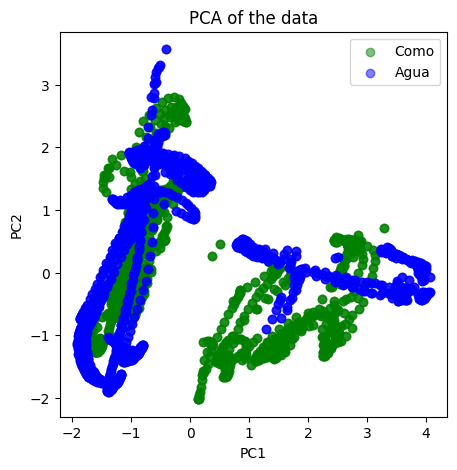
\includegraphics[width=0.5\textwidth]{figuras/PCA-ComoAgua.png}
    \caption{Análisis de similitud entre las clases \textit{como} y \textit{agua}}
    \label{fig:PCA-ComoAgua}
\end{figure}

En la Figura \ref{fig:PCA-ComoBeber} se puede observar que las clases \textit{como} y \textit{beber} tienen cierto grado de similitud en los movimientos de ambas manos.
Esto puede dificultar la distinción entre ellas, ya que el modelo puede confundir los movimientos de ambas manos.

\begin{figure}[H]
    \centering
    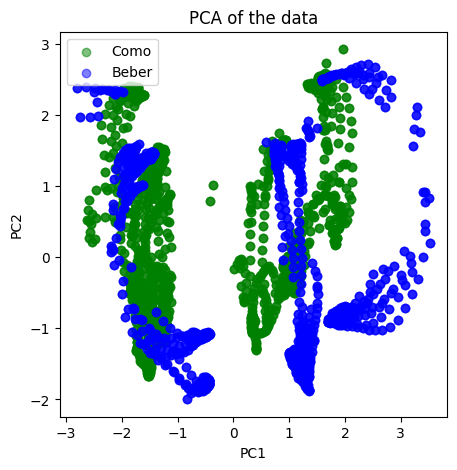
\includegraphics[width=0.5\textwidth]{figuras/PCA-ComoBeber.png}
    \caption{Análisis de similitud entre las clases \textit{como} y \textit{beber}}
    \label{fig:PCA-ComoBeber}
\end{figure}

En la Figura \ref{fig:PCA-CuandoDonde} se puede observar que las clases \textit{cuando} y \textit{donde} tienen un bajo grado de similitud en los movimientos de ambas manos.
Sin embargo, en el análisis de similitud se observa que las clases tienen cierto grado de superposición, lo cual puede dificultar la distinción entre ellas.

\begin{figure}[H]
    \centering
    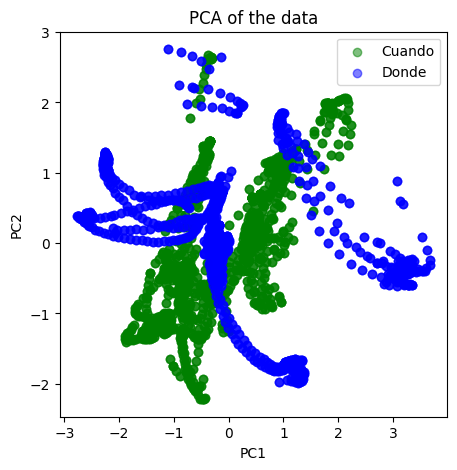
\includegraphics[width=0.45\textwidth]{figuras/PCA-CuandoDonde.png}
    \caption{Análisis de similitud entre las clases \textit{cuando} y \textit{donde}}
    \label{fig:PCA-CuandoDonde}
\end{figure}

En la Figura \ref{fig:PCA-SedQuien} se puede observar que las clases \textit{sed} y \textit{quien} tienen un bajo grado de similitud en los movimientos de ambas manos.
El análisis de similitud no muestra una superposición significativa entre las clases, lo cual indica que el modelo puede confundir las clases debido a otros factores.

\begin{figure}[H]
    \centering
    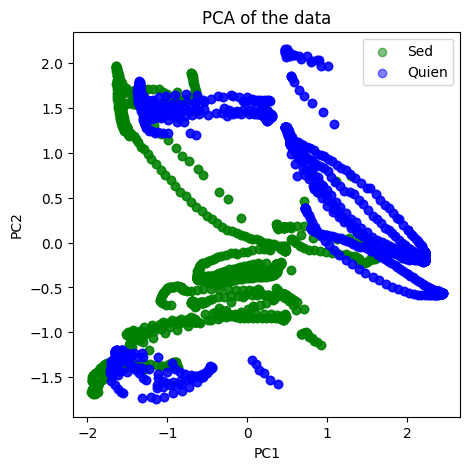
\includegraphics[width=0.45\textwidth]{figuras/PCA-SedQuien.png}
    \caption{Análisis de similitud entre las clases \textit{sed} y \textit{quien}}
    \label{fig:PCA-SedQuien}
\end{figure}

Adicional a esto, se realizó un análisis de similitud entre todas las clases, con el objetivo de identificar otras clases que puedan tener un alto grado de similitud.
En la Figura \ref{fig:PCA-AllClasses} se puede observar el análisis de similitud entre todas las clases.

\begin{figure}[H]
    \centering
    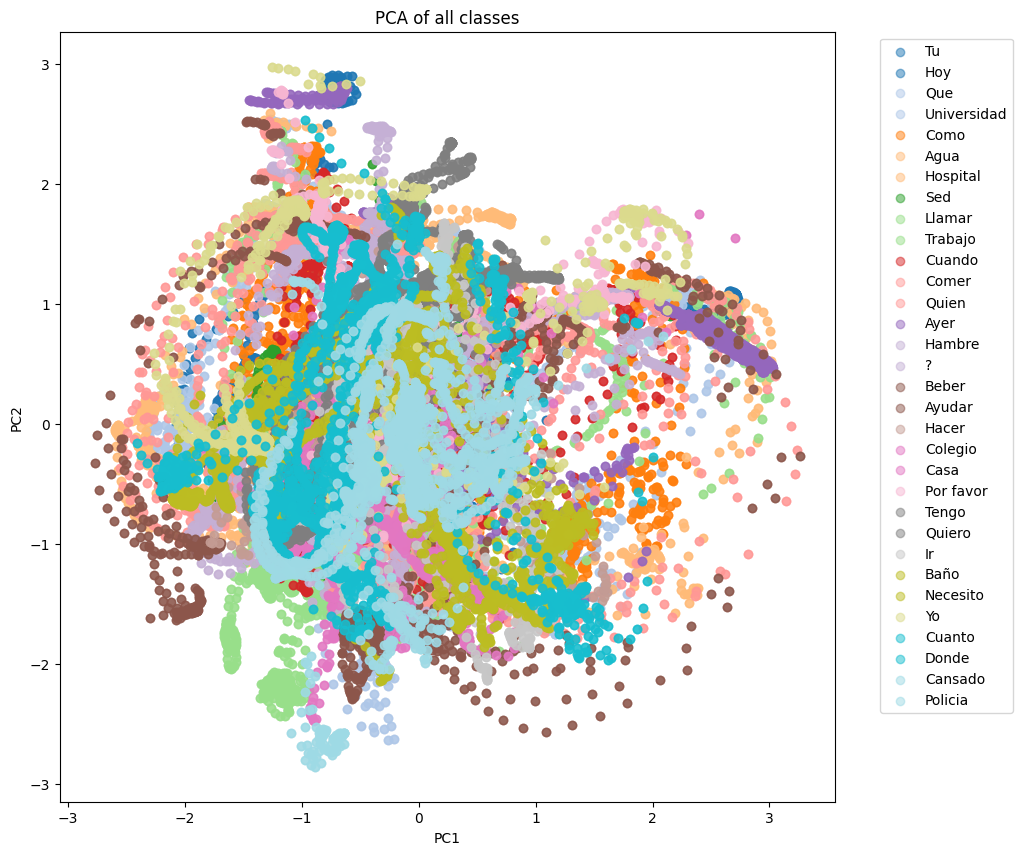
\includegraphics[width=0.8\textwidth]{figuras/PCA-All.png}
    \caption{Análisis de similitud entre todas las clases}
    \label{fig:PCA-AllClasses}
\end{figure}

Por último, se validó el balance de las clases en el conjunto de datos de entrenamiento.
La Figura \ref{fig:ClasesBalanceadas} muestra el balance de las clases en el conjunto de datos de entrenamiento.

\begin{figure}[H]
    \centering
    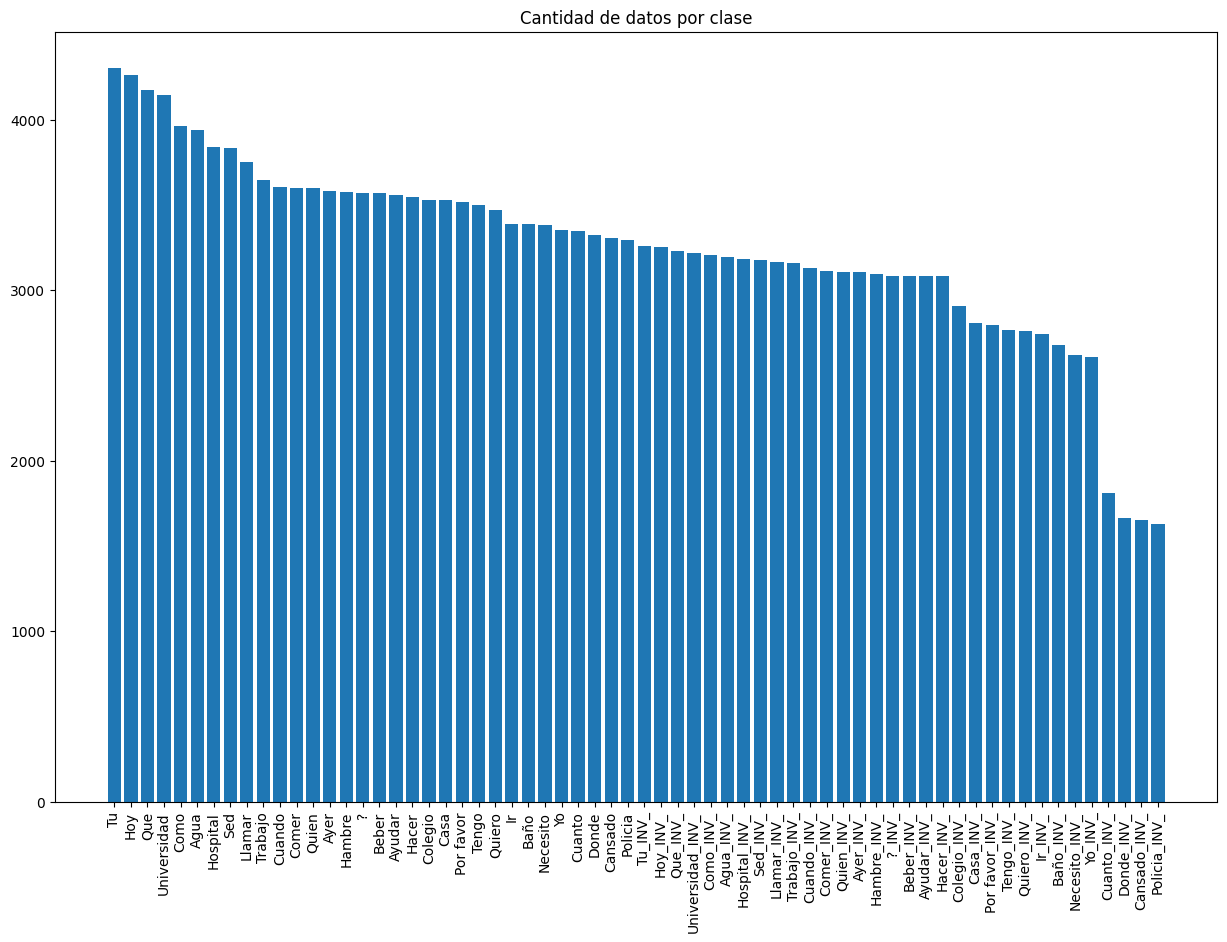
\includegraphics[width=0.7\textwidth]{figuras/DataBalance.png}
    \caption{Balance de clases en el conjunto de datos de entrenamiento}
    \label{fig:ClasesBalanceadas}
\end{figure}

\subsection{Proceso iterativo de desarrollo del modelo}
El proceso de desarrollo del modelo de reconocimiento de lengua de señas de Guatemala fue iterativo, siguiendo la metodología propuesta para el proyecto.
En total, se realizaron 8 iteraciones, en las cuales se crearon modelos distintos y se evaluaron utilizando el conjunto de prueba.
Todos los modelos fueron entrenados con 25 épocas, utilizando un tamaño de lote de 32 y un optimizador Adam. 
A continuación se presentan los modelos resultantes de cada iteración, junto con su desempeño en el conjunto de prueba.

\subsubsection{Modelo base}
La composición del modelo base se puede observar en la Figura \ref{fig:ModeloInicial}. 
Este modelo tiene una capa de entrada, cuatro capas densas con activación tangente hiperbólica y una capa de salida con activación softmax.

\begin{figure}[H]
    \centering
    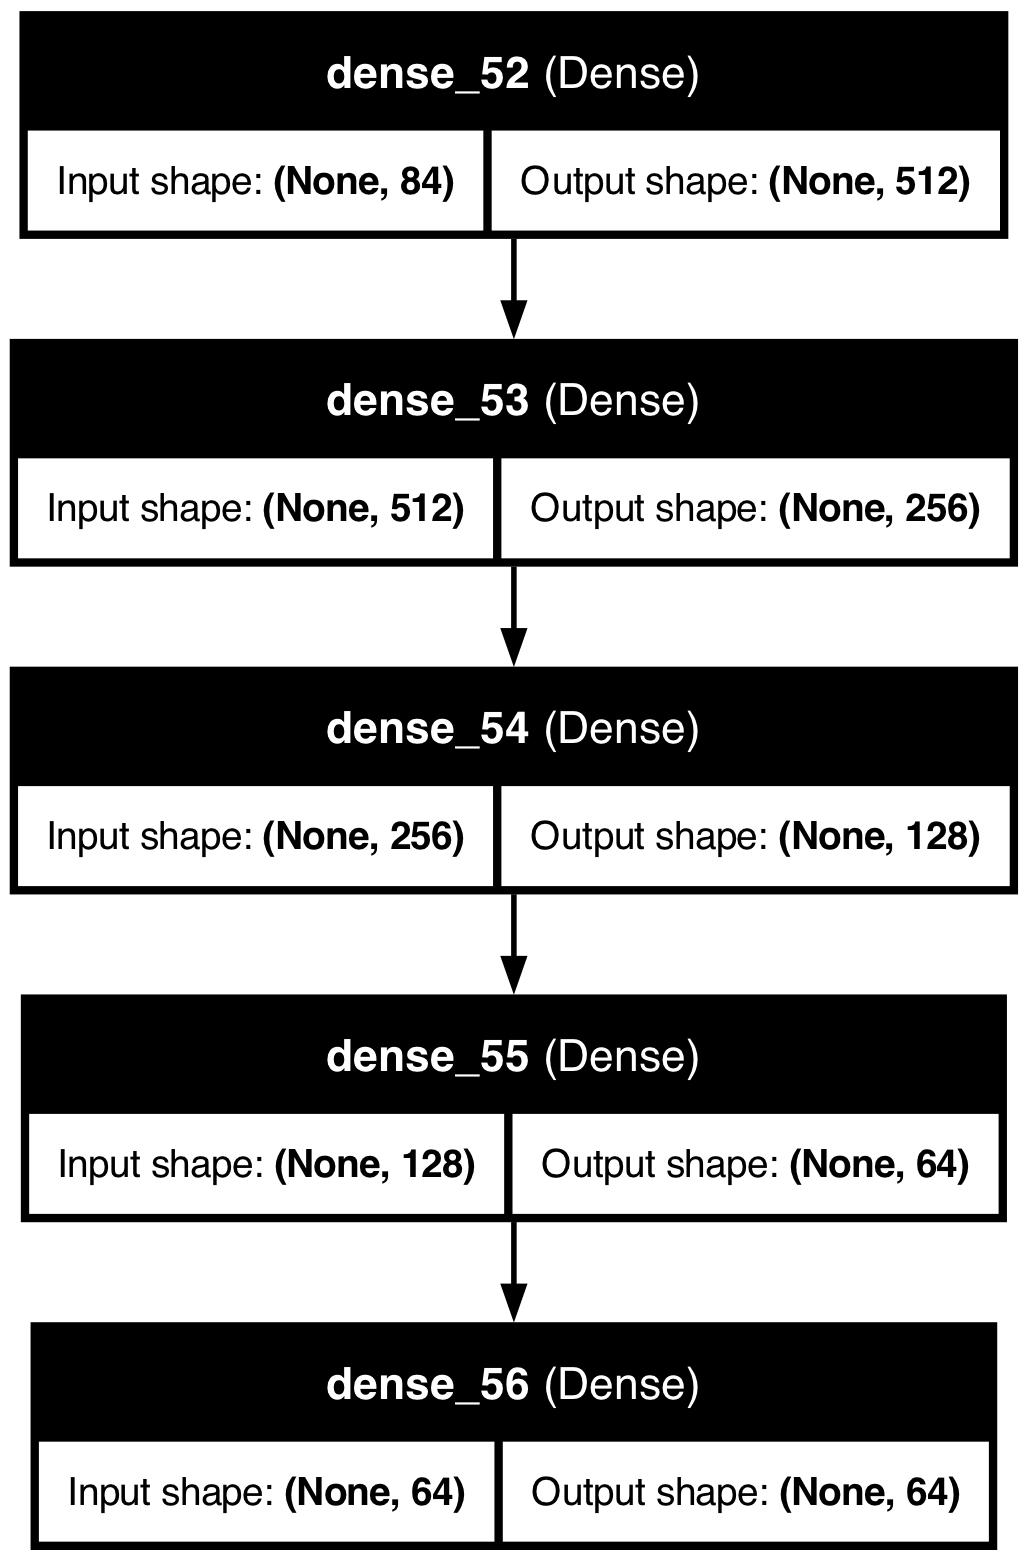
\includegraphics[width=0.5\textwidth]{figuras/baseModel.png}
    \caption{Modelo inicial}
    \label{fig:ModeloInicial}
\end{figure}

El desempeño del modelo inicial se puede observar en la tabla \ref{tab:DesempeñoModeloInicial}.
Este modelo inicial tiene una precisión de 0.7708, una sensibilidad de 0.8822 y un F1 de 0.8895.
Adicional a esto, se puede observar la matriz de confusión en la Figura \ref{fig:CMModeloInicial} y el historial de entrenamiento en la Figura \ref{fig:HistoryModeloInicial}.

\begin{figure}[H]
    \centering
    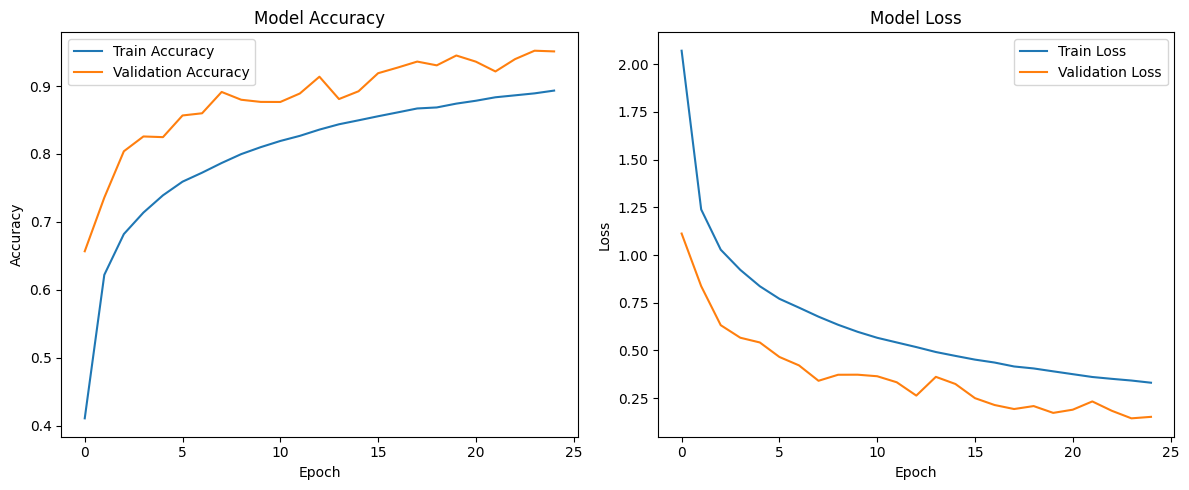
\includegraphics[width=0.8\textwidth]{figuras/baseModelHistory.png}
    \caption{Historial de entrenamiento del modelo base}
    \label{fig:HistoryModeloInicial}
\end{figure}

\begin{table}[H]
    \centering
    \begin{tabular}{|c|c|}
        \hline
        \textbf{Métrica} & \textbf{Valor} \\
        \hline
        Precisión & 0.7708 \\
        \hline
        Sensibilidad & 0.8822 \\
        \hline
        F1 & 0.8895 \\
        \hline
    \end{tabular}
    \caption{Desempeño del modelo base}
    \label{tab:DesempeñoModeloInicial}
\end{table}

\begin{figure}[H]
    \centering
    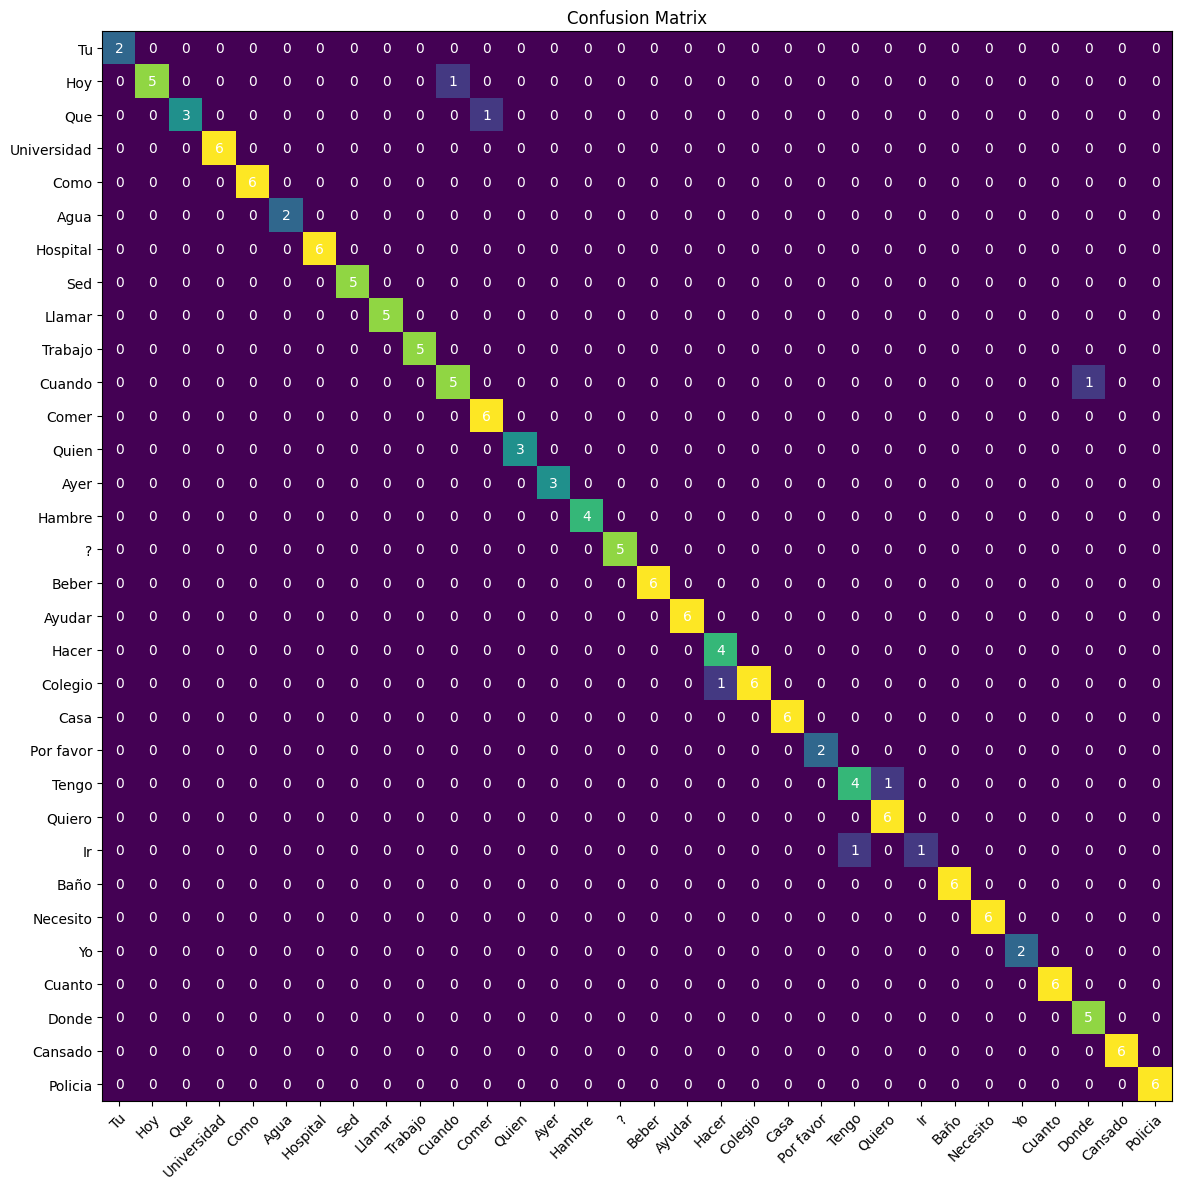
\includegraphics[width=0.8\textwidth]{figuras/baseModelCM.png}
    \caption{Matriz de confusión del modelo base}
    \label{fig:CMModeloInicial}
\end{figure}

\subsubsection{Aumento de complejidad del modelo base}
En la iteración previa, se observó que el modelo base tenía un desempeño aceptable, pero se consideró que la arquitectura del modelo era muy simple.
En esta iteración, se aumentó la complejidad del modelo base, añadiendo dos capas densas adicionales con activación tangente hiperbólica.
Estas capas adicionales tienen 2048 y 1024 neuronas, respectivamente.

La composición del modelo con aumento de complejidad se puede observar en la Figura \ref{fig:ModeloComplejo}.
Este modelo tiene una capa de entrada, seis capas densas con activación tangente hiperbólica y una capa de salida con activación softmax.

\begin{figure}[H]
    \centering
    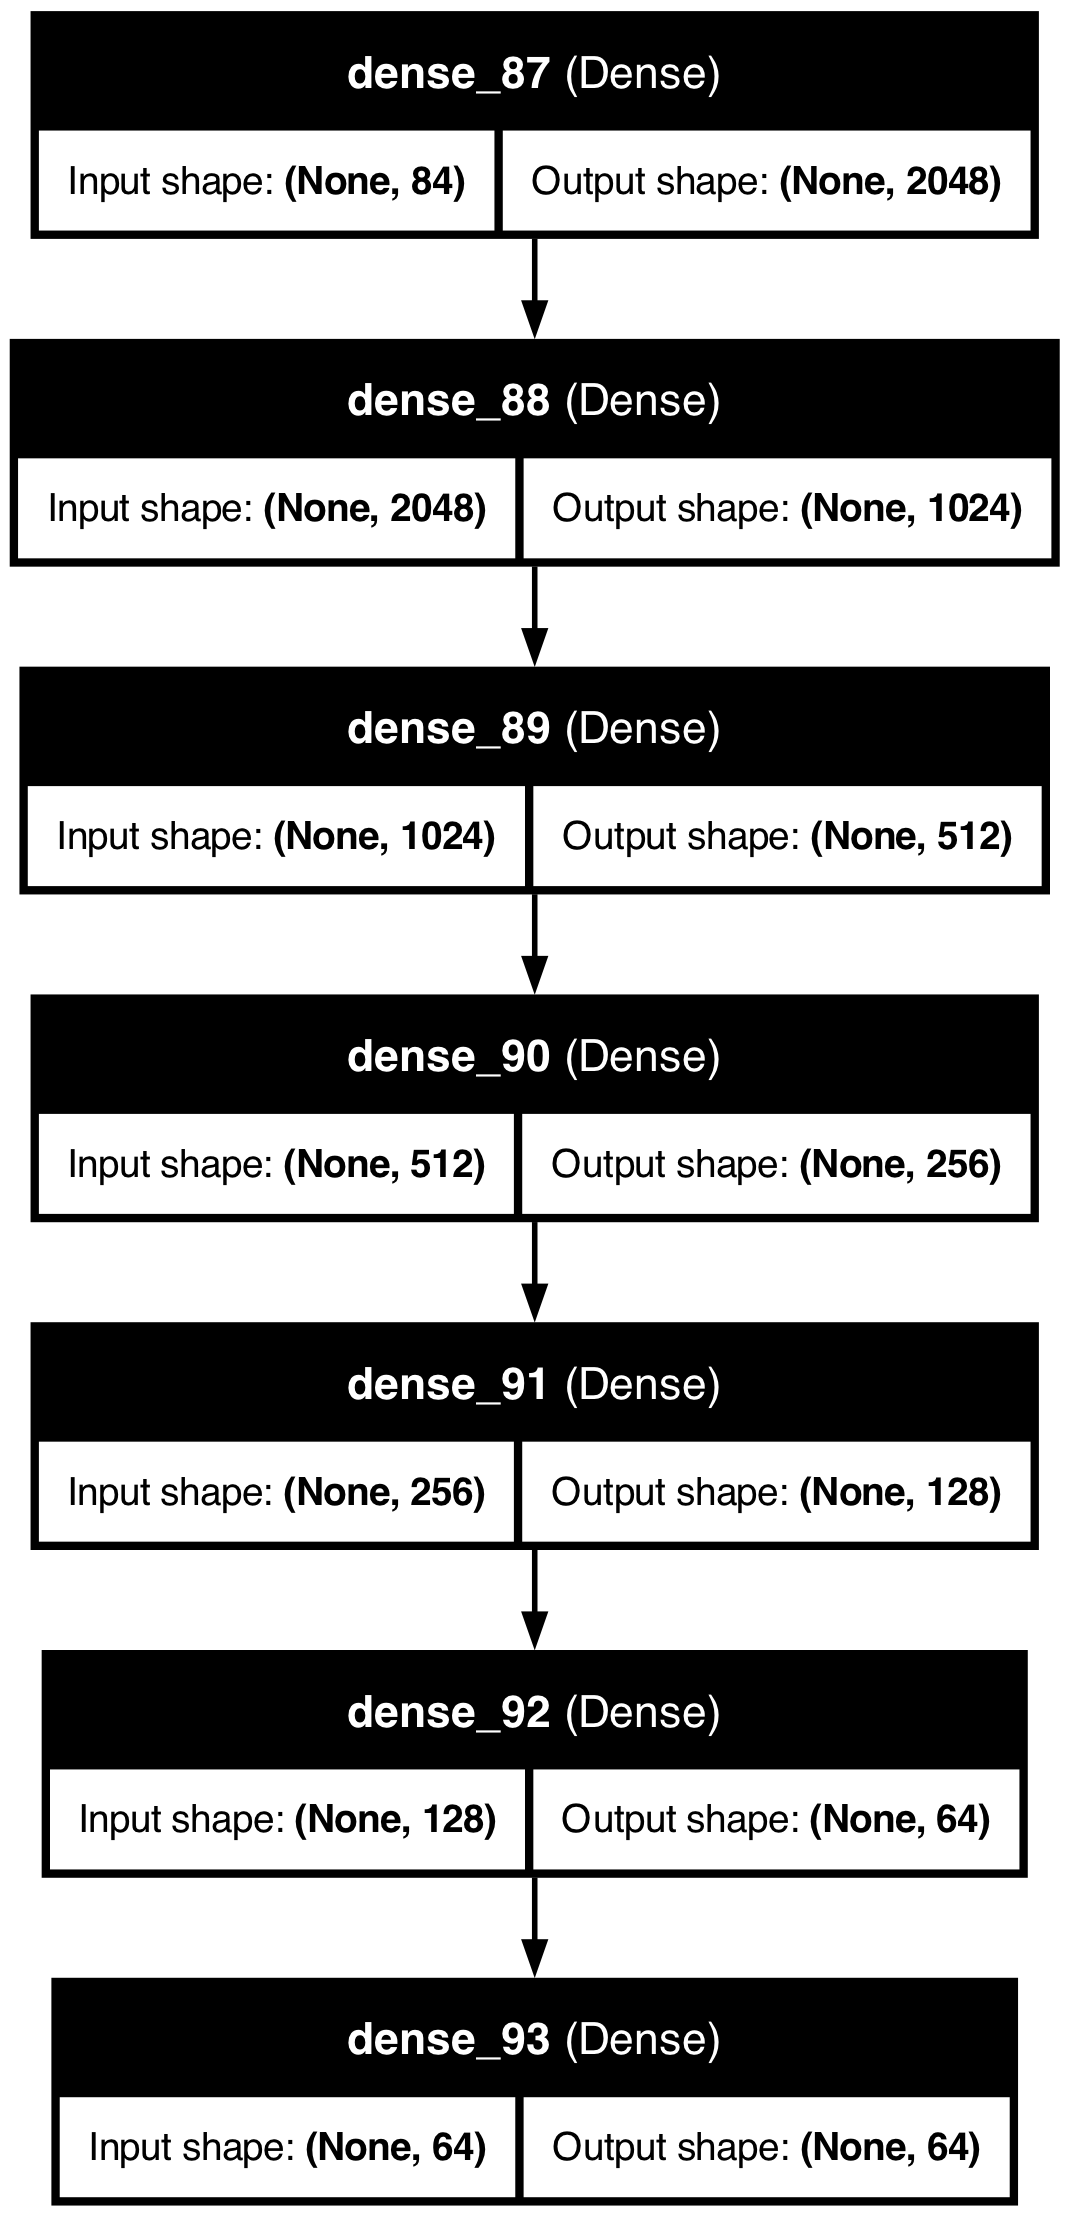
\includegraphics[width=0.45\textwidth]{figuras/modelComplex.png}
    \caption{Modelo con aumento de complejidad}
    \label{fig:ModeloComplejo}
\end{figure}

El desempeño de este modelo se puede observar en la tabla \ref{tab:DesempeñoModeloComplejo}.
Este modelo tiene una precisión de 0.5937, una sensibilidad de 0.8957 y un F1 de 0.9026.
Adicional a esto, se puede observar la matriz de confusión en la Figura \ref{fig:CMModeloComplejo} y el historial de entrenamiento en la Figura \ref{fig:HistoryModeloComplejo}.

\begin{figure}[H]
    \centering
    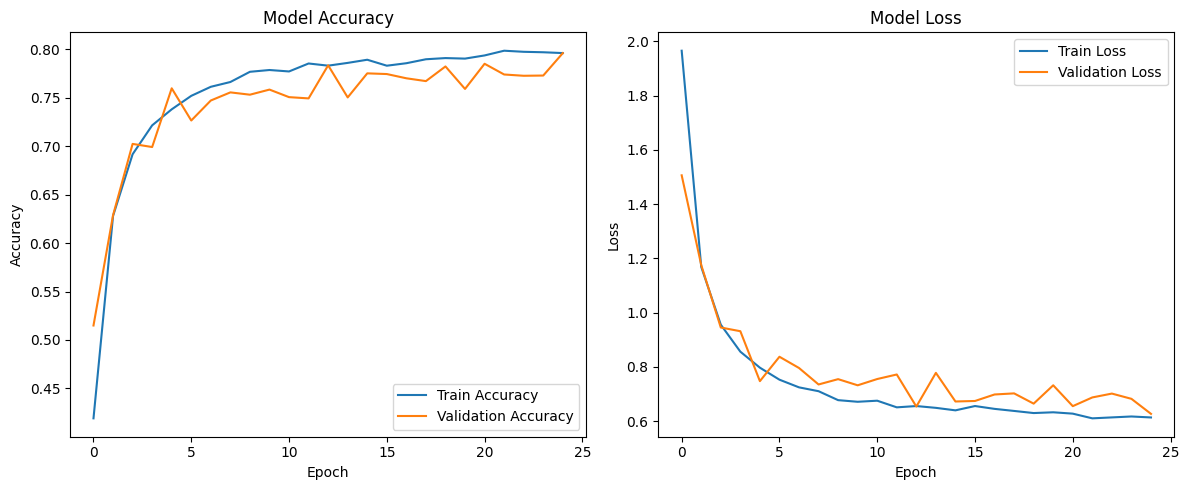
\includegraphics[width=0.8\textwidth]{figuras/modelComplexHistory.png}
    \caption{Historial de entrenamiento del modelo con aumento de complejidad}
    \label{fig:HistoryModeloComplejo}
\end{figure}

\begin{table}[H]
    \centering
    \begin{tabular}{|c|c|}
        \hline
        \textbf{Métrica} & \textbf{Valor} \\
        \hline
        Precisión & 0.5937 \\
        \hline
        Sensibilidad & 0.8957 \\
        \hline
        F1 & 0.9026 \\
        \hline
    \end{tabular}
    \caption{Desempeño del modelo con aumento de complejidad}
    \label{tab:DesempeñoModeloComplejo}
\end{table}

\begin{figure}[H]
    \centering
    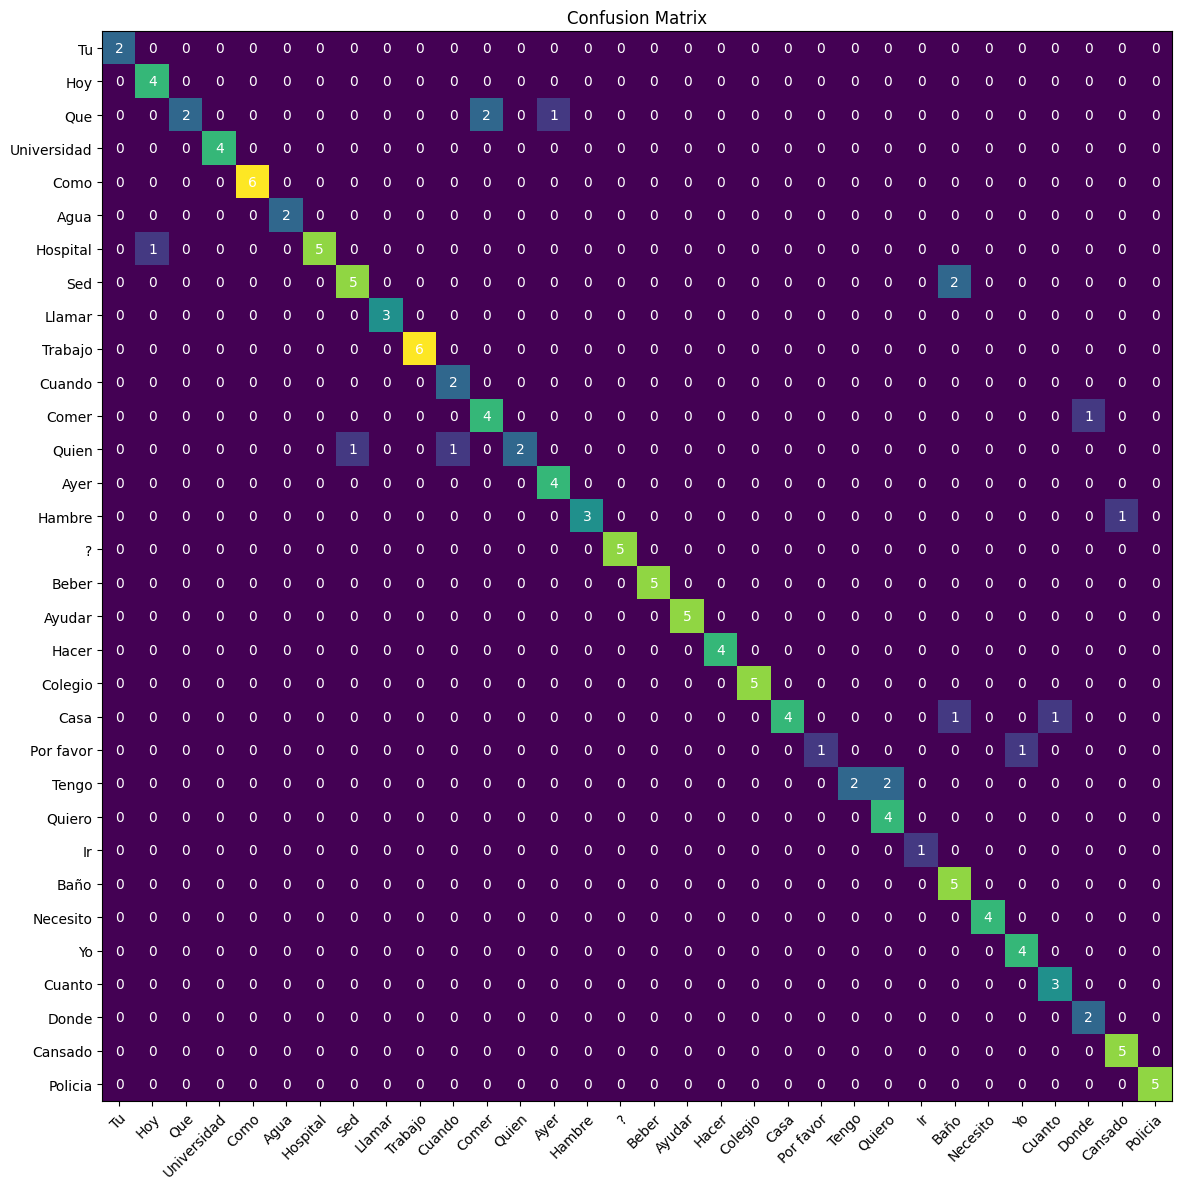
\includegraphics[width=0.8\textwidth]{figuras/modelComplexCM.png}
    \caption{Matriz de confusión del modelo con aumento de complejidad}
    \label{fig:CMModeloComplejo}
\end{figure}

\subsubsection{Adición de dropout al modelo base}
La composición del modelo base con dropout se puede observar en la Figura \ref{fig:ModeloBaseDropout}.
Este modelo tiene una capa de entrada, cuatro capas densas con activación tangente hiperbólica y una capa de salida con activación softmax.
Adicional a esto, se ha añadido una capa de dropout con una tasa de 0.1 a cada capa densa.

\begin{figure}[H]
    \centering
    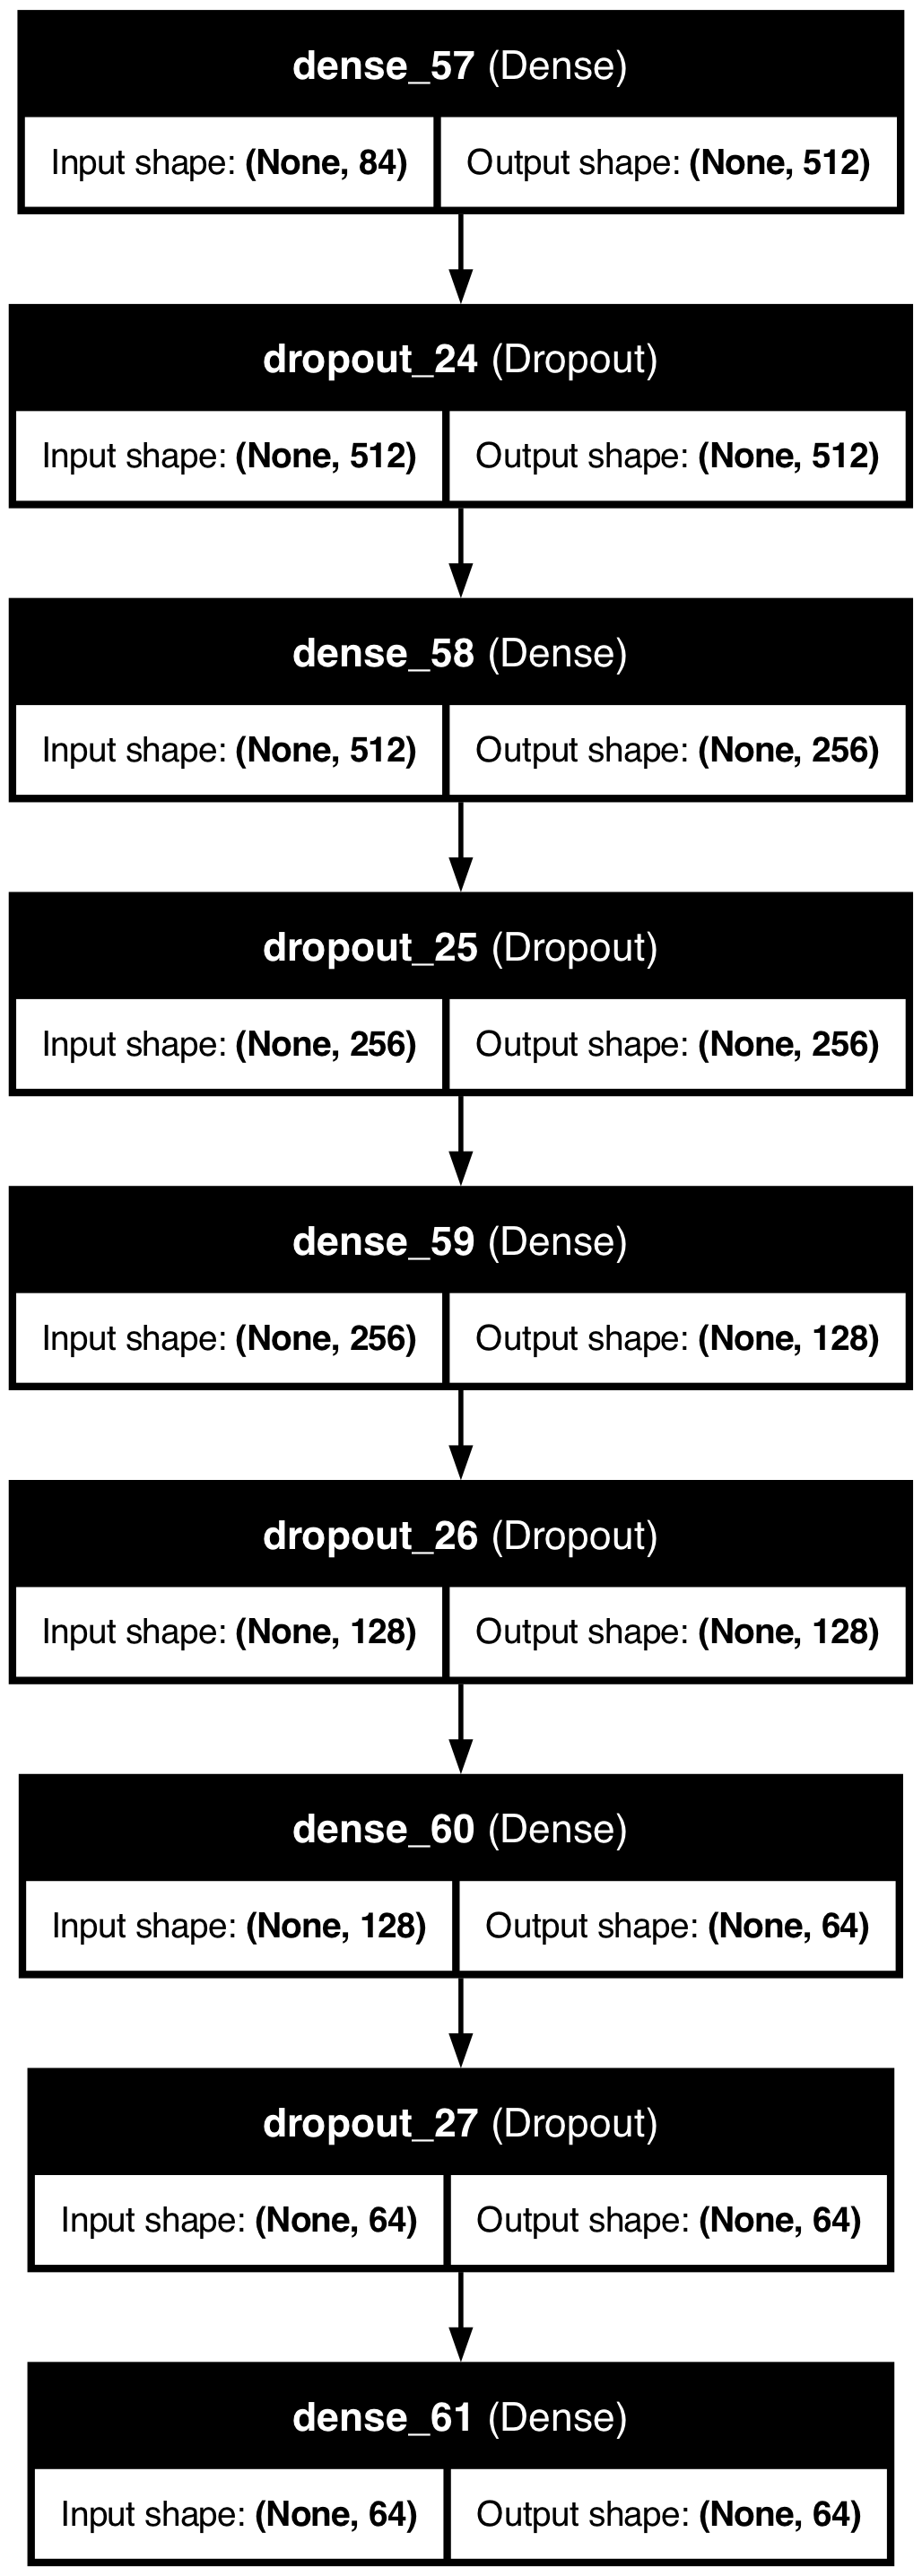
\includegraphics[width=0.4\textwidth]{figuras/modelDropout.png}
    \caption{Modelo base con dropout}
    \label{fig:ModeloBaseDropout}
\end{figure}

El desempeño de este modelo se puede observar en la tabla \ref{tab:DesempeñoModeloBaseDropout}.
Este modelo tiene una precisión de 0.8072, una sensibilidad de 0.9247 y un F1 de 0.9274.
Adicional a esto, se puede observar la matriz de confusión en la Figura \ref{fig:CMModeloBaseDropout} y el historial de entrenamiento en la Figura \ref{fig:HistoryModeloBaseDropout}.

\begin{figure}[H]
    \centering
    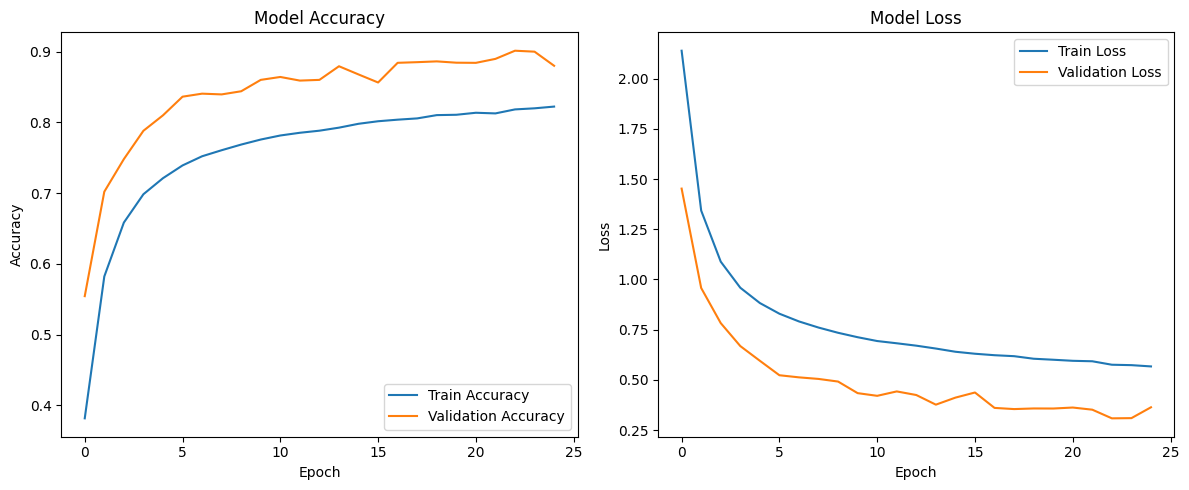
\includegraphics[width=0.8\textwidth]{figuras/modelDropoutHistory.png}
    \caption{Historial de entrenamiento del modelo base con dropout}
    \label{fig:HistoryModeloBaseDropout}
\end{figure}

\begin{table}[H]
    \centering
    \begin{tabular}{|c|c|}
        \hline
        \textbf{Métrica} & \textbf{Valor} \\
        \hline
        Precisión & 0.8072 \\
        \hline
        Sensibilidad & 0.9247 \\
        \hline
        F1 & 0.9274 \\
        \hline
    \end{tabular}
    \caption{Desempeño del modelo base con dropout}
    \label{tab:DesempeñoModeloBaseDropout}
\end{table}

\begin{figure}[H]
    \centering
    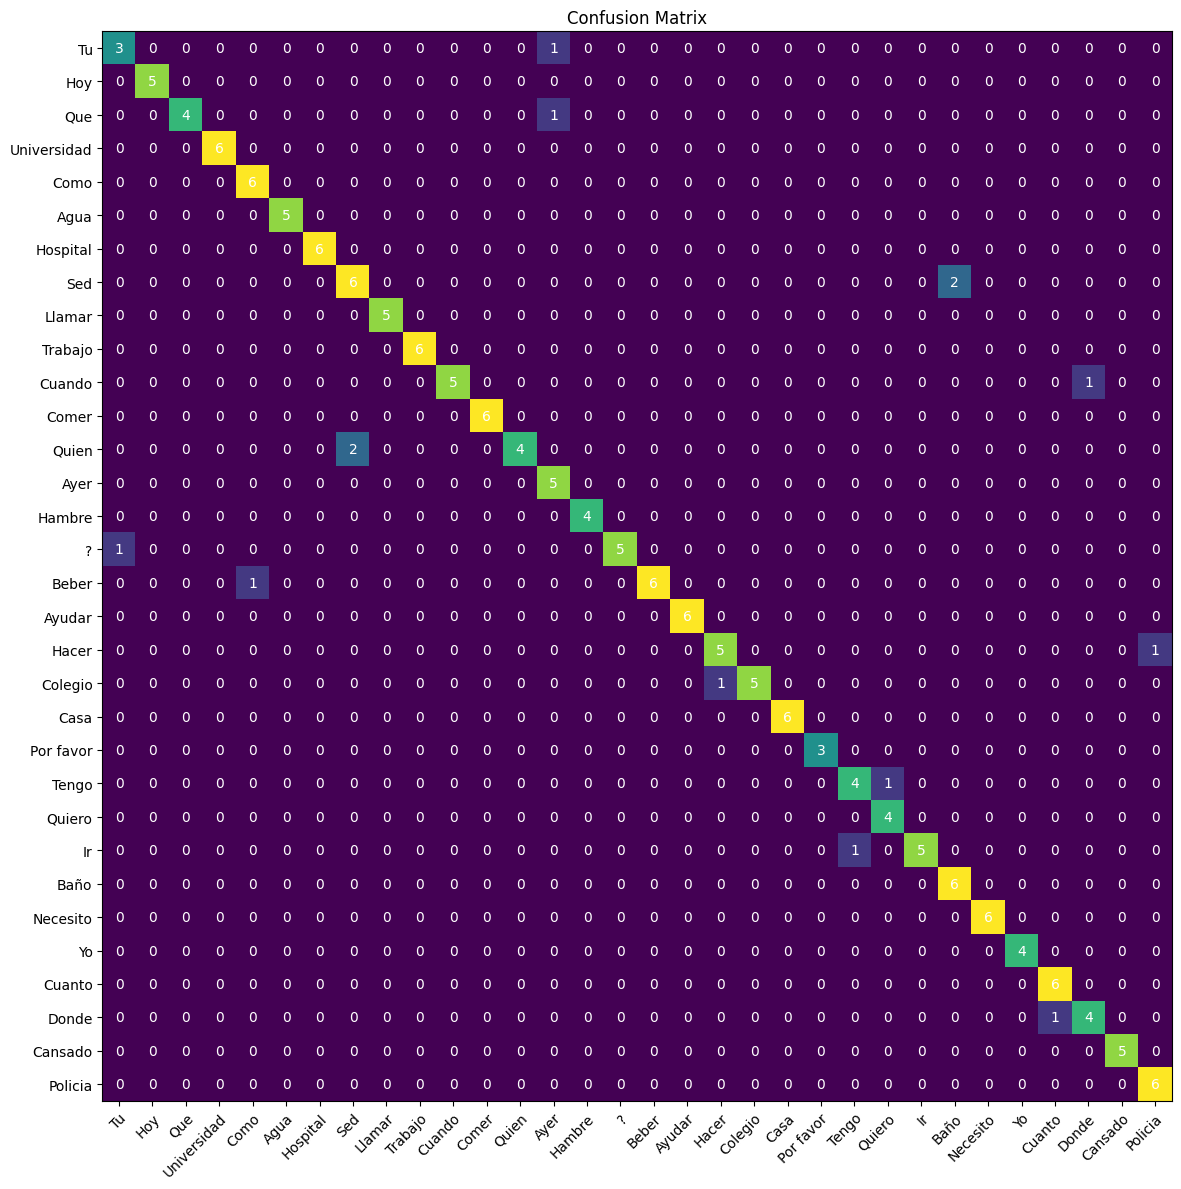
\includegraphics[width=0.8\textwidth]{figuras/modelDropoutCM.png}
    \caption{Matriz de confusión del modelo base con dropout}
    \label{fig:CMModeloBaseDropout}
\end{figure}

\subsubsection{Fine-tuning de las capas dropout}
En la iteración previa, se observó que la adición de dropout al modelo base mejoró el desempeño del modelo.
Esto se debe a que el dropout ayuda a prevenir el sobreajuste del modelo, al desactivar aleatoriamente un porcentaje de las neuronas en cada época, lo cual permite que el modelo generalice mejor.
En esta iteración, se realizó un fine-tuning de la tasa de dropout, con el objetivo de encontrar la tasa de dropout que maximizara el desempeño del modelo.
Se realizan pruebas con dos modelos distintos, con el objetivo de encontrar la tasa de dropout que maximice el desempeño del modelo.

La composición del primero de los modelos se puede observar en la Figura \ref{fig:ModeloDropoutV2}.
Este modelo tiene una capa de entrada, cuatro capas densas con activación tangente hiperbólica y una capa de salida con activación softmax.
A diferencia del modelo anterior, este modelo tiene una capa de dropout con una tasa de 0.2 a cada capa densa.

\begin{figure}[H]
    \centering
    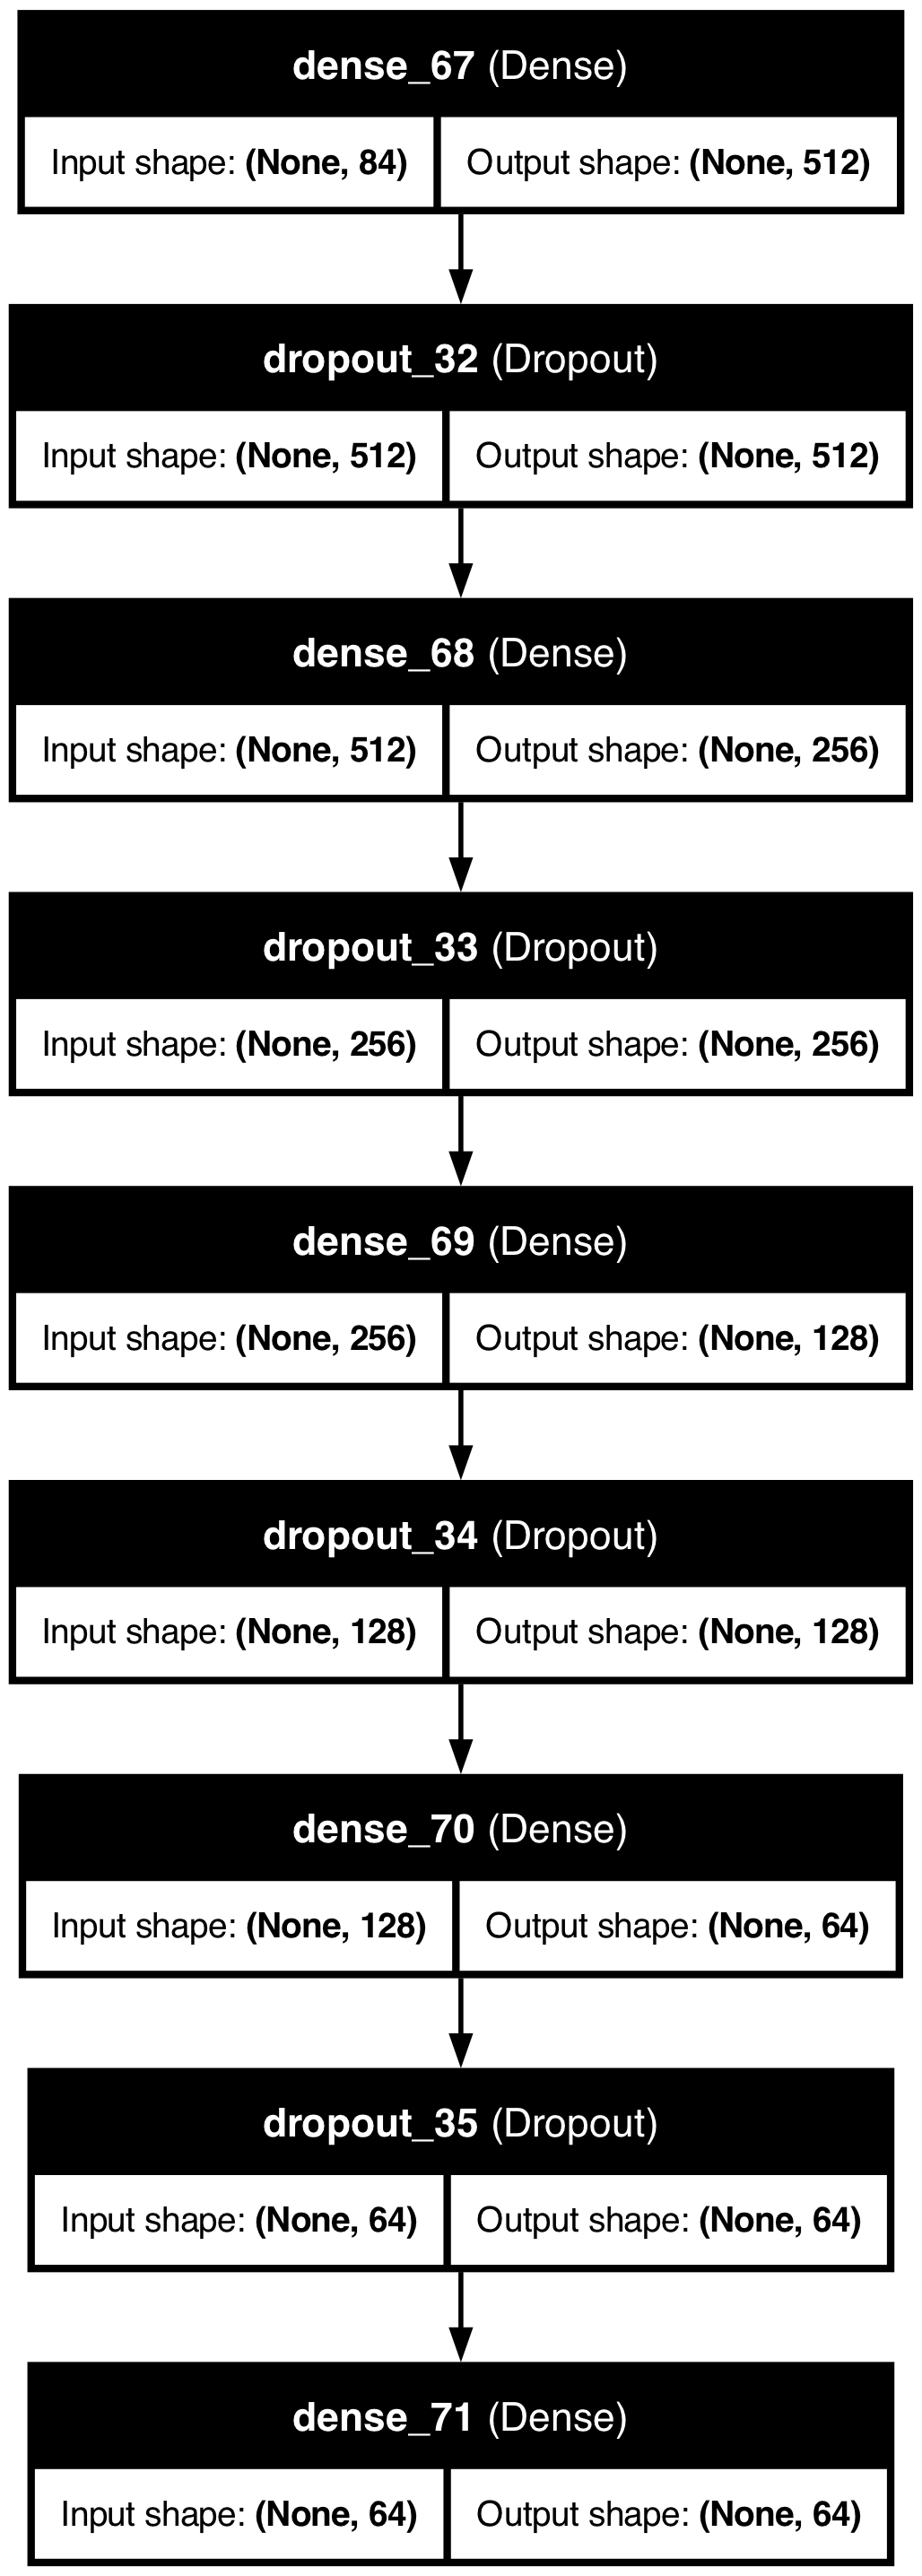
\includegraphics[width=0.375\textwidth]{figuras/modelDropoutV2.png}
    \caption{Primera iteración de fine tuning de la tasa de dropout}
    \label{fig:ModeloDropoutV2}
\end{figure}

El desempeño de este modelo se puede observar en la tabla \ref{tab:DesempeñoModeloDropoutV2}.
Este modelo tiene una precisión de 0.7656, una sensibilidad de 0.9681 y un F1 de 0.9617.
Adicional a esto, se puede observar la matriz de confusión en la Figura \ref{fig:CMModeloDropoutV2} y el historial de entrenamiento en la Figura \ref{fig:HistoryModeloDropoutV2}.

\begin{figure}[H]
    \centering
    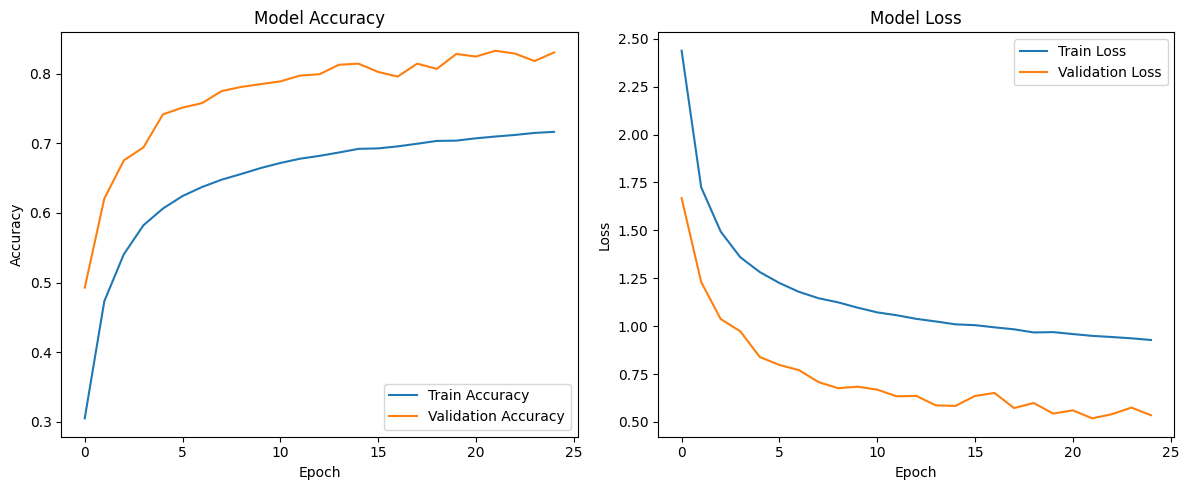
\includegraphics[width=0.7\textwidth]{figuras/modelDropoutV2History.png}
    \caption{Historial de entrenamiento del primer modelo de fine tuning de la tasa de dropout}
    \label{fig:HistoryModeloDropoutV2}
\end{figure}

\begin{table}[H]
    \centering
    \begin{tabular}{|c|c|}
        \hline
        \textbf{Métrica} & \textbf{Valor} \\
        \hline
        Precisión & 0.7656 \\
        \hline
        Sensibilidad & 0.9681 \\
        \hline
        F1 & 0.9617 \\
        \hline
    \end{tabular}
    \caption{Desempeño del primer modelo de fine tuning de la tasa de dropout}
    \label{tab:DesempeñoModeloDropoutV2}
\end{table}

\begin{figure}[H]
    \centering
    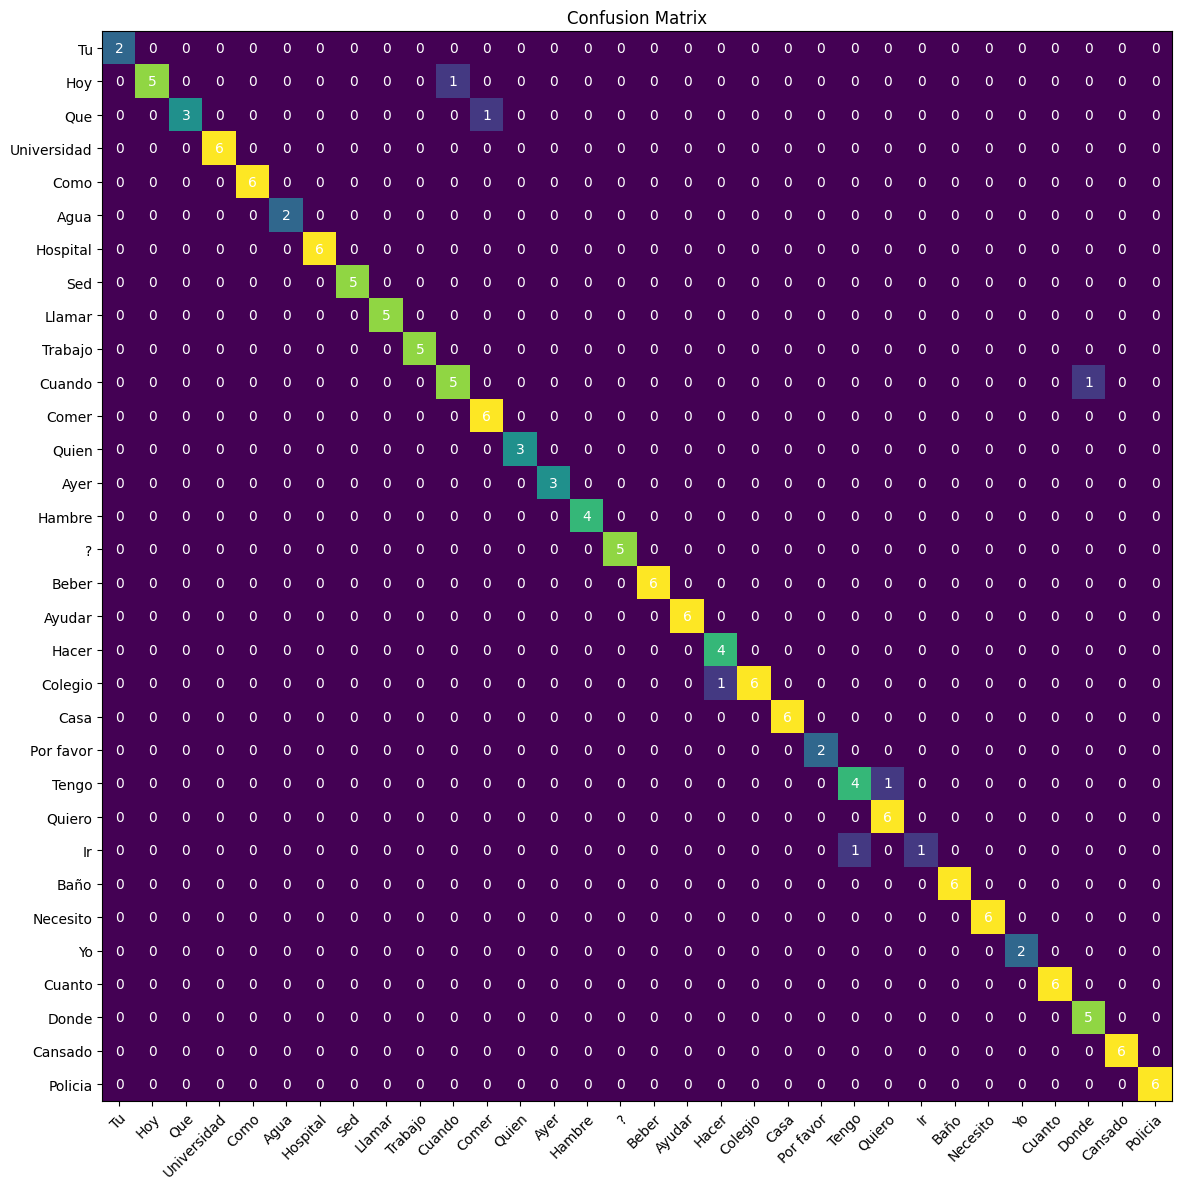
\includegraphics[width=0.7\textwidth]{figuras/modelDropoutV2CM.png}
    \caption{Matriz de confusión del primer modelo de fine tuning de la tasa de dropout}
    \label{fig:CMModeloDropoutV2}
\end{figure}

La composición del segundo de los modelos se puede observar en la Figura \ref{fig:ModeloDropoutV3}.
Este modelo tiene una capa de entrada, cuatro capas densas con activación tangente hiperbólica y una capa de salida con activación softmax.
Debido a que el modelo anterior tuvo un desempeño inferior al modelo base con dropout, se decidió probar con dos capas de dropout con una tasa de 0.2 y dos capas de dropout con una tasa de 0.1.

\begin{figure}[H]
    \centering
    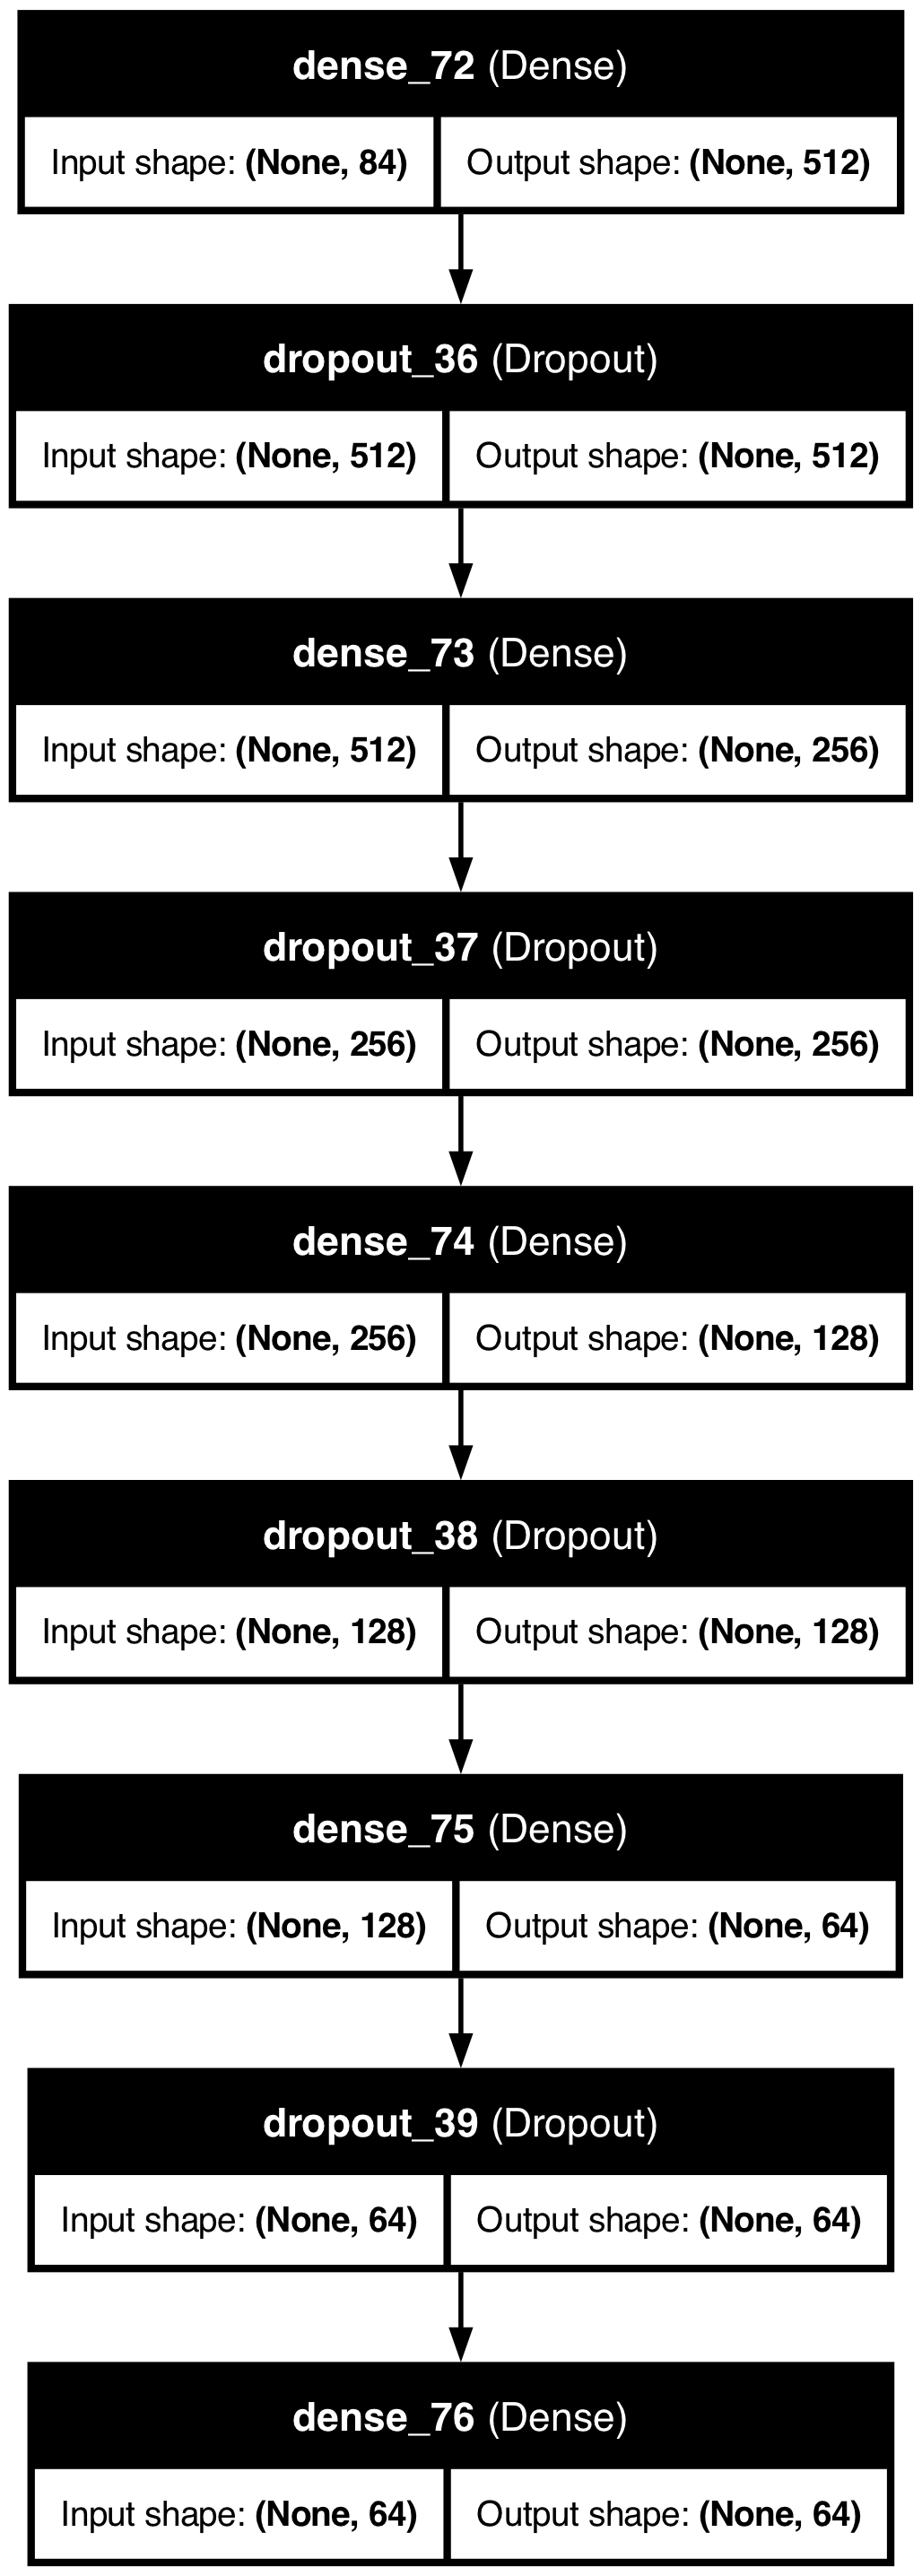
\includegraphics[width=0.45\textwidth]{figuras/modelDropoutV3.png}
    \caption{Segunda iteración de fine tuning de la tasa de dropout}
    \label{fig:ModeloDropoutV3}
\end{figure}

El desempeño de este modelo se puede observar en la tabla \ref{tab:DesempeñoModeloDropoutV3}.
Este modelo tiene una precisión de 0.7708, una sensibilidad de 0.9541 y un F1 de 0.9543.
Adicional a esto, se puede observar la matriz de confusión en la Figura \ref{fig:CMModeloDropoutV3} y el historial de entrenamiento en la Figura \ref{fig:HistoryModeloDropoutV3}.

\begin{figure}[H]
    \centering
    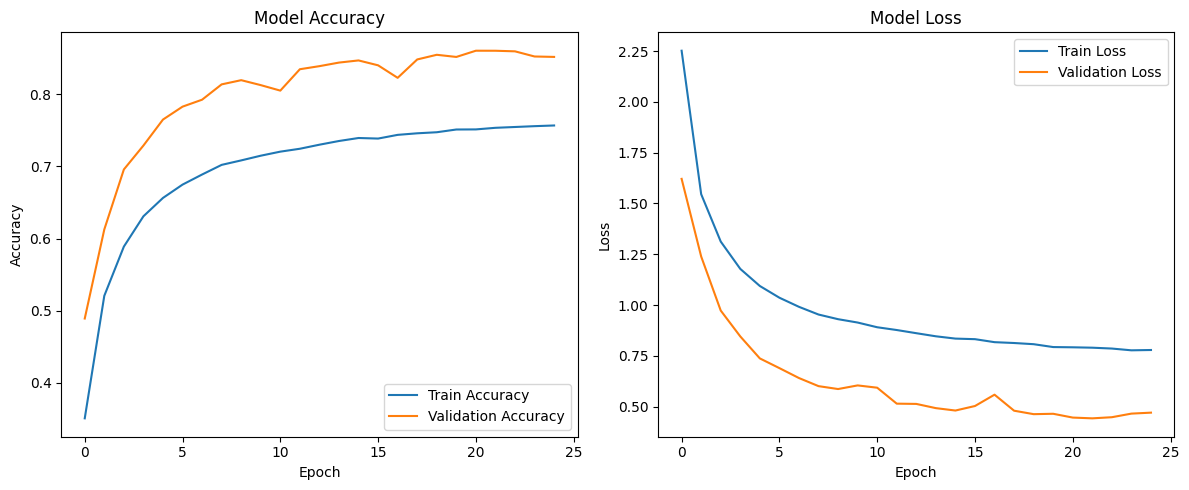
\includegraphics[width=0.7\textwidth]{figuras/modelDropoutV3History.png}
    \caption{Historial de entrenamiento del segundo modelo de fine tuning de la tasa de dropout}
    \label{fig:HistoryModeloDropoutV3}
\end{figure}

\begin{table}[H]
    \centering
    \begin{tabular}{|c|c|}
        \hline
        \textbf{Métrica} & \textbf{Valor} \\
        \hline
        Precisión & 0.7708 \\
        \hline
        Sensibilidad & 0.9541 \\
        \hline
        F1 & 0.9543 \\
        \hline
    \end{tabular}
    \caption{Desempeño del segundo modelo de fine tuning de la tasa de dropout}
    \label{tab:DesempeñoModeloDropoutV3}
\end{table}

\begin{figure}[H]
    \centering
    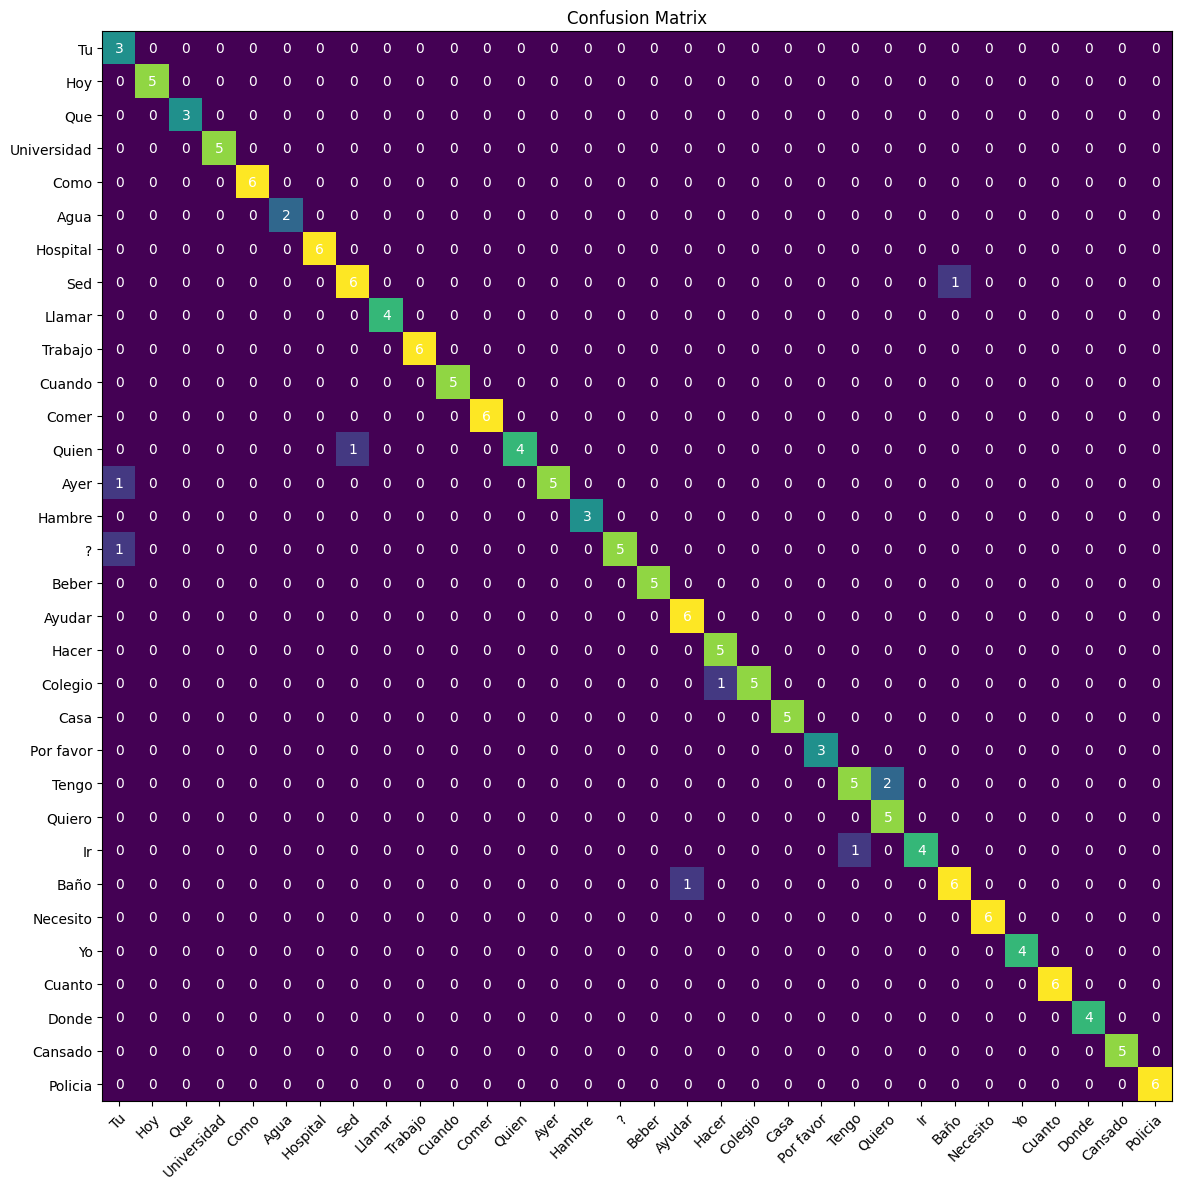
\includegraphics[width=0.7\textwidth]{figuras/modelDropoutV3CM.png}
    \caption{Matriz de confusión del segundo modelo de fine tuning de la tasa de dropout}
    \label{fig:CMModeloDropoutV3}
\end{figure}

\subsubsection{Adición de normalización por lotes al modelo base}

La normalización por lotes es una técnica que se utiliza para normalizar las entradas de una red neuronal, con el objetivo de acelerar el proceso de entrenamiento y mejorar la precisión del modelo.
En esta iteración, se añadió una capa de normalización por lotes por cada capa densa del modelo base, con el objetivo de evaluar si la normalización por lotes mejoraba el desempeño del modelo.
La composición del modelo con normalización por lotes se puede observar en la Figura \ref{fig:ModeloBatchNormalization}.

\begin{figure}[H]
    \centering
    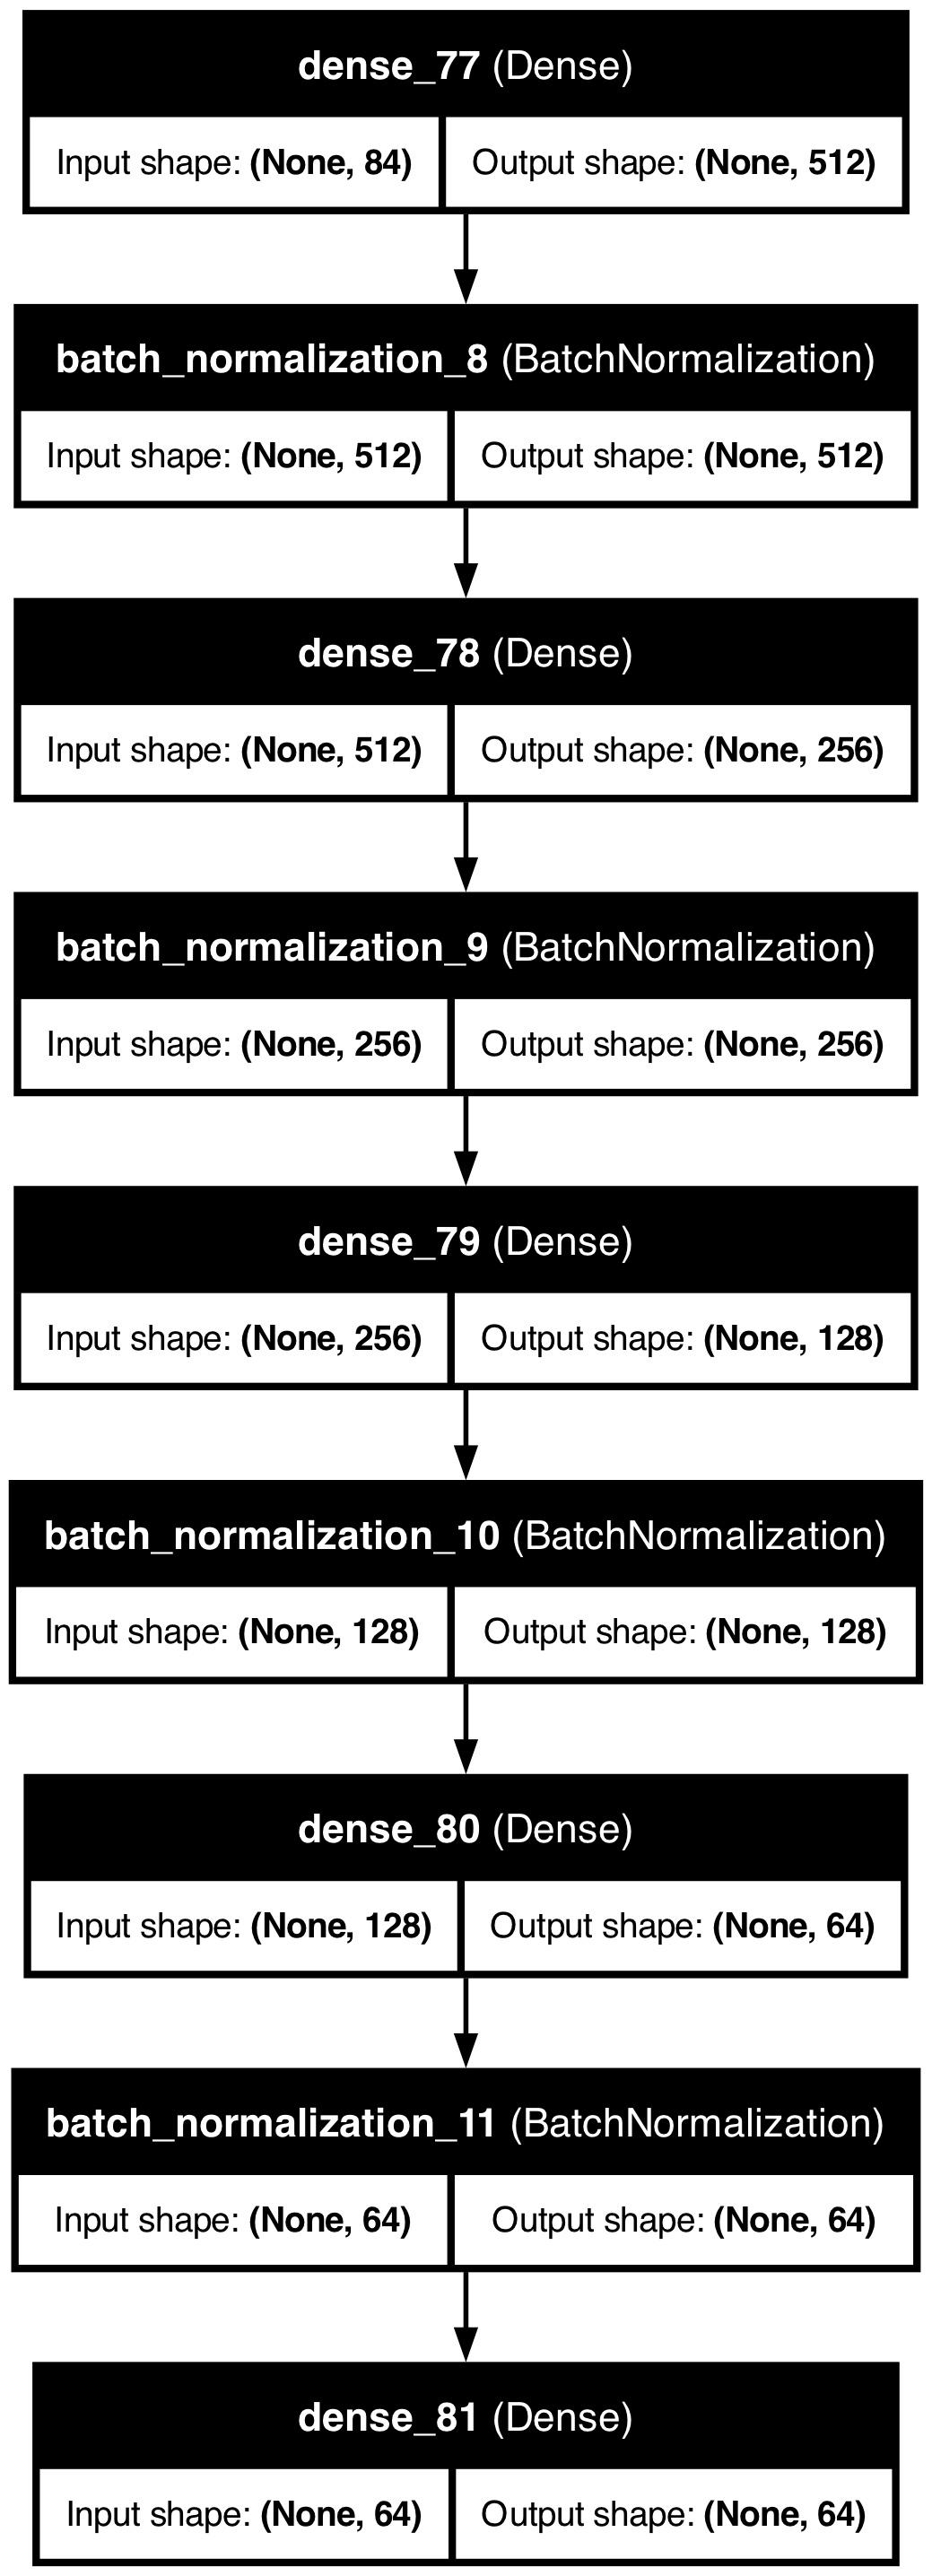
\includegraphics[width=0.425\textwidth]{figuras/modelBN.png}
    \caption{Modelo con normalización por lotes}
    \label{fig:ModeloBatchNormalization}
\end{figure}

El desempeño de este modelo se puede observar en la tabla \ref{tab:DesempeñoModeloBatchNormalization}.
Este modelo tiene una precisión de 0.8593, una sensibilidad de 0.9136 y un F1 de 0.9155.
Adicional a esto, se puede observar la matriz de confusión en la Figura \ref{fig:CMModeloBatchNormalization} y el historial de entrenamiento en la Figura \ref{fig:HistoryModeloBatchNormalization}.

\begin{figure}[H]
    \centering
    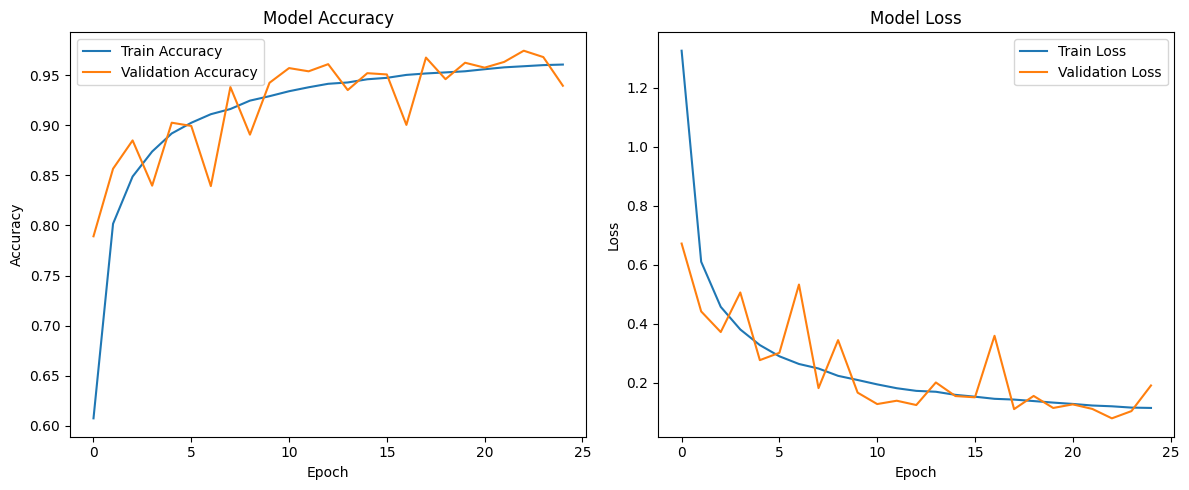
\includegraphics[width=0.7\textwidth]{figuras/modelBNHistory.png}
    \caption{Historial de entrenamiento del modelo con normalización por lotes}
    \label{fig:HistoryModeloBatchNormalization}
\end{figure}

\begin{table}[H]
    \centering
    \begin{tabular}{|c|c|}
        \hline
        \textbf{Métrica} & \textbf{Valor} \\
        \hline
        Precisión & 0.8593 \\
        \hline
        Sensibilidad & 0.9136 \\
        \hline
        F1 & 0.9155 \\
        \hline
    \end{tabular}
    \caption{Desempeño del modelo con normalización por lotes}
    \label{tab:DesempeñoModeloBatchNormalization}
\end{table}

\begin{figure}[H]
    \centering
    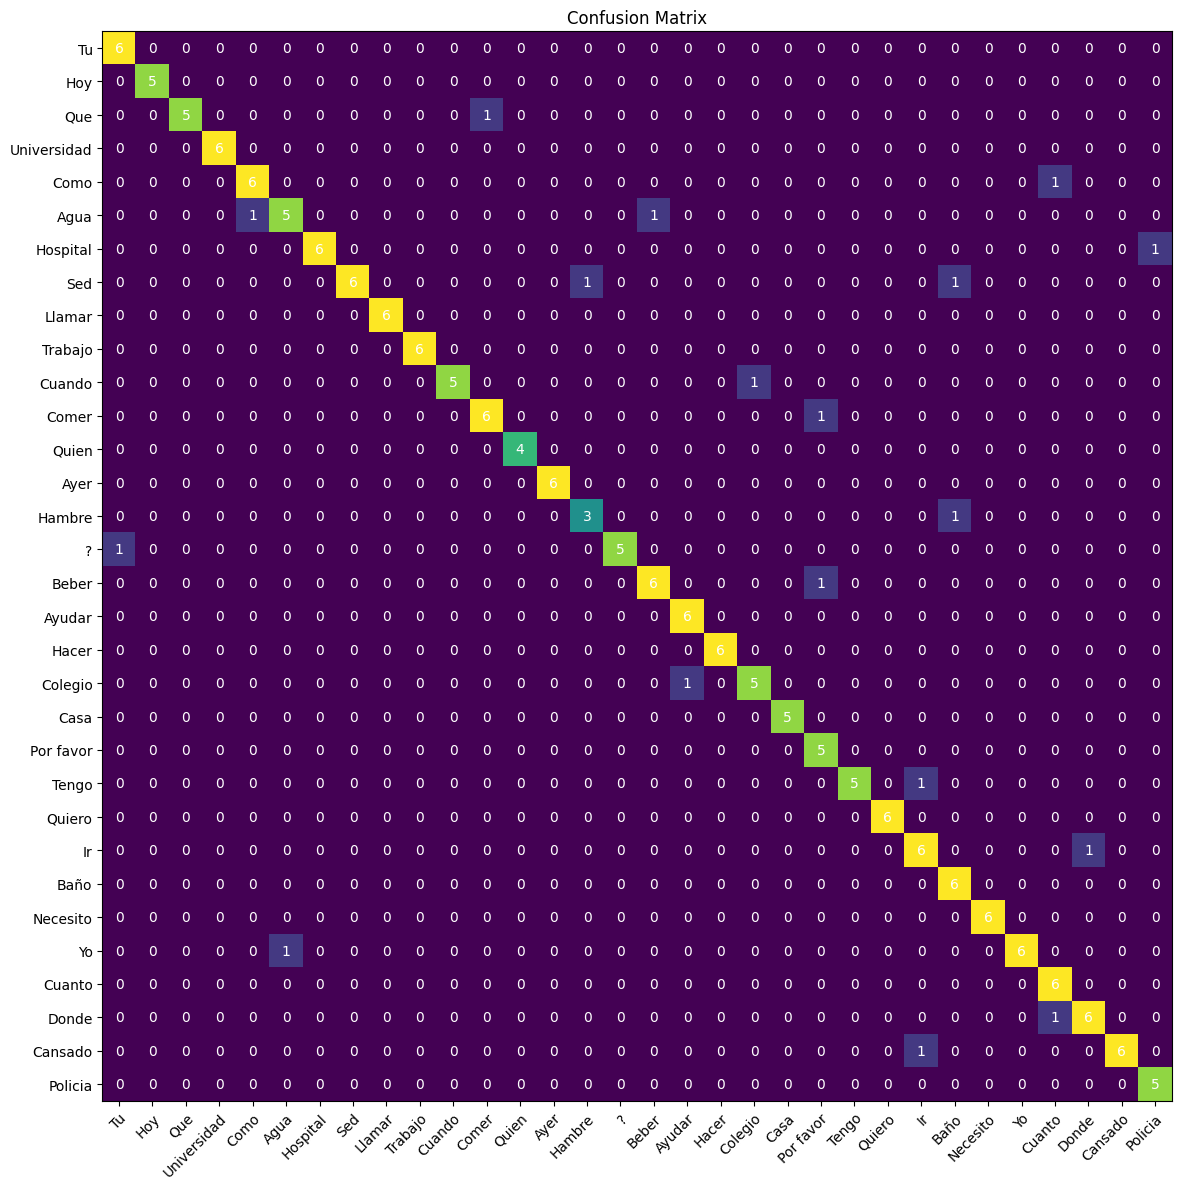
\includegraphics[width=0.7\textwidth]{figuras/modelBNCM.png}
    \caption{Matriz de confusión del modelo con normalización por lotes}
    \label{fig:CMModeloBatchNormalization}
\end{figure}

\subsubsection{Combinación de dropout y normalización por lotes}

En esta iteración, se combinaron las técnicas de dropout y normalización por lotes, con el objetivo de evaluar si la combinación de ambas técnicas mejoraba el desempeño del modelo.
Se realizan pruebas con dos modelos distintos, con el objetivo de encontrar la combinación de dropout y normalización por lotes que maximizara el desempeño del modelo.
La composición del primero de los modelos se puede observar en la Figura \ref{fig:ModeloDropoutBN}.

\begin{figure}[H]
    \centering
    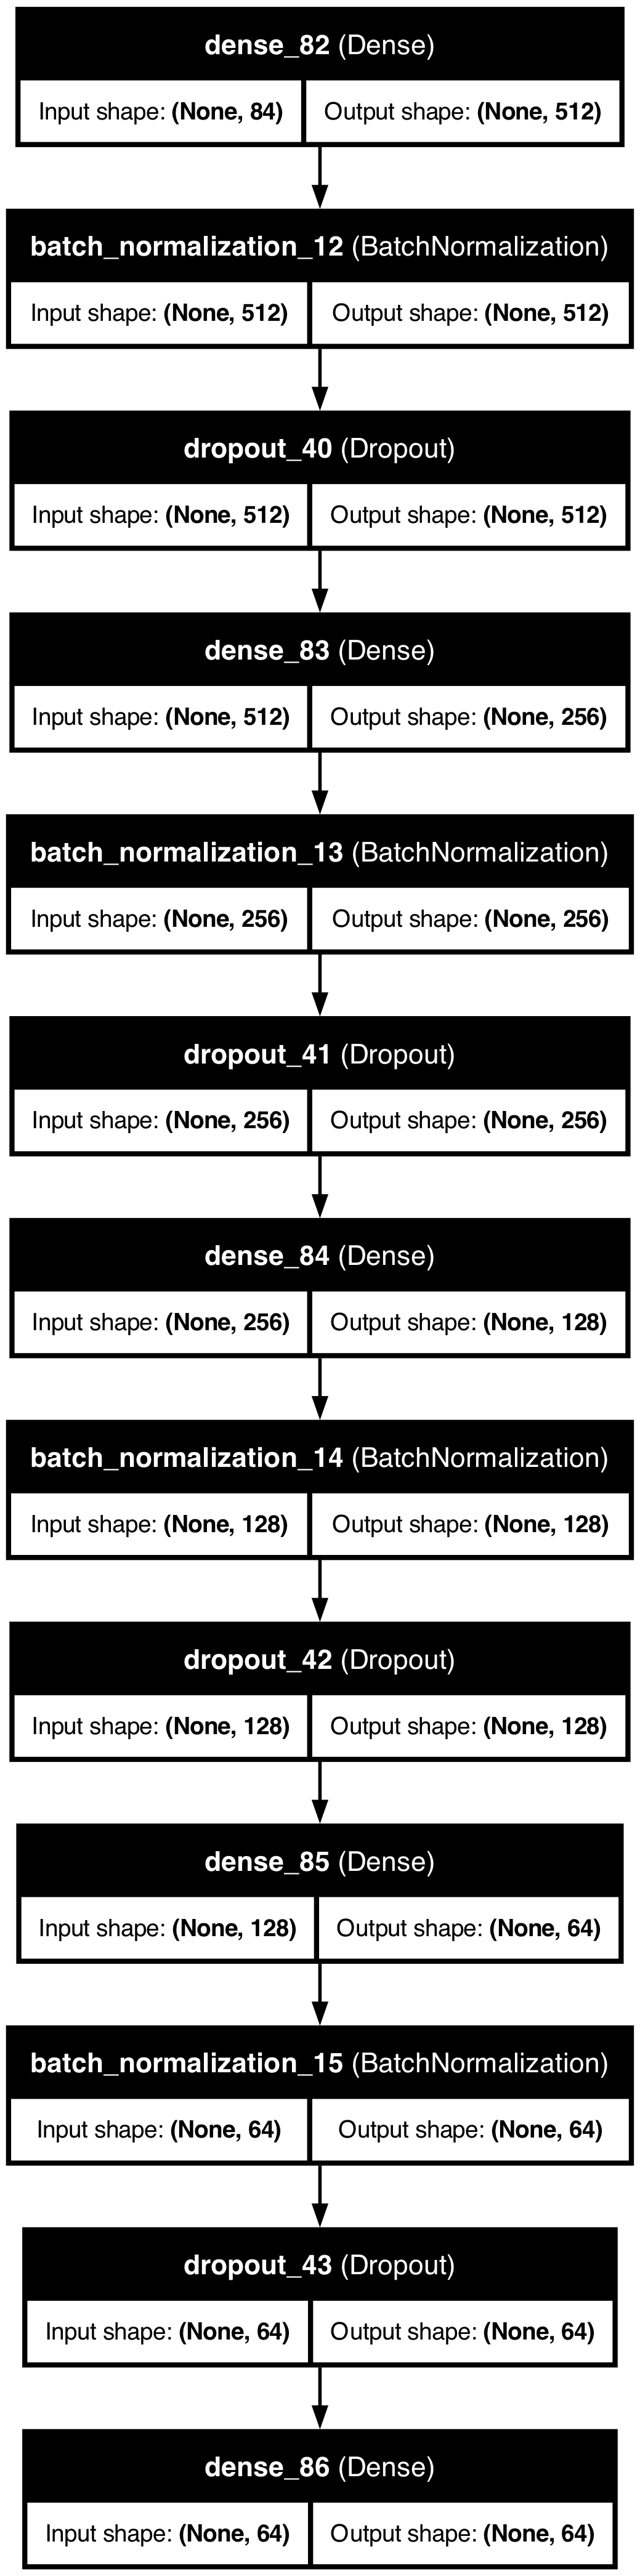
\includegraphics[width=0.3\textwidth]{figuras/modelDropoutBN.png}
    \caption{Primer modelo con dropout y normalización por lotes}
    \label{fig:ModeloDropoutBN}
\end{figure}

El desempeño de este modelo se puede observar en la tabla \ref{tab:DesempeñoModeloDropoutBN}.
Este modelo tiene una precisión de 0.8593, una sensibilidad de 0.9461 y un F1 de 0.9441.
Adicional a esto, se puede observar la matriz de confusión en la Figura \ref{fig:CMModeloDropoutBN} y el historial de entrenamiento en la Figura \ref{fig:HistoryModeloDropoutBN}.

\begin{figure}[H]
    \centering
    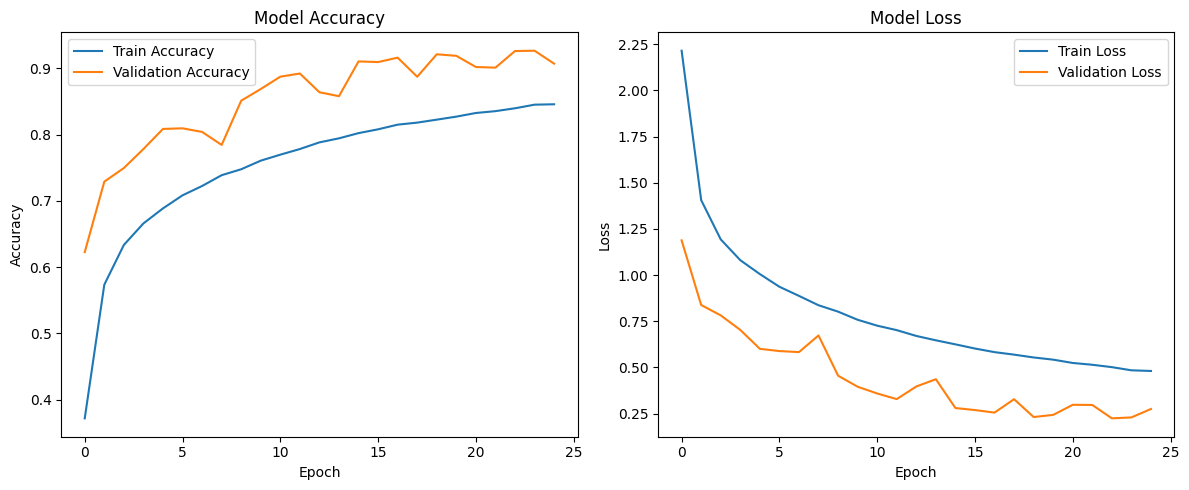
\includegraphics[width=0.7\textwidth]{figuras/modelDropoutBNHistory.png}
    \caption{Historial de entrenamiento del primer modelo con de dropout y normalización por lotes}
    \label{fig:HistoryModeloDropoutBN}
\end{figure}

\begin{table}[H]
    \centering
    \begin{tabular}{|c|c|}
        \hline
        \textbf{Métrica} & \textbf{Valor} \\
        \hline
        Precisión & 0.8593 \\
        \hline
        Sensibilidad & 0.9461 \\
        \hline
        F1 & 0.9441 \\
        \hline
    \end{tabular}
    \caption{Desempeño del primer modelo con dropout y normalización por lotes}
    \label{tab:DesempeñoModeloDropoutBN}
\end{table}

\begin{figure}[H]
    \centering
    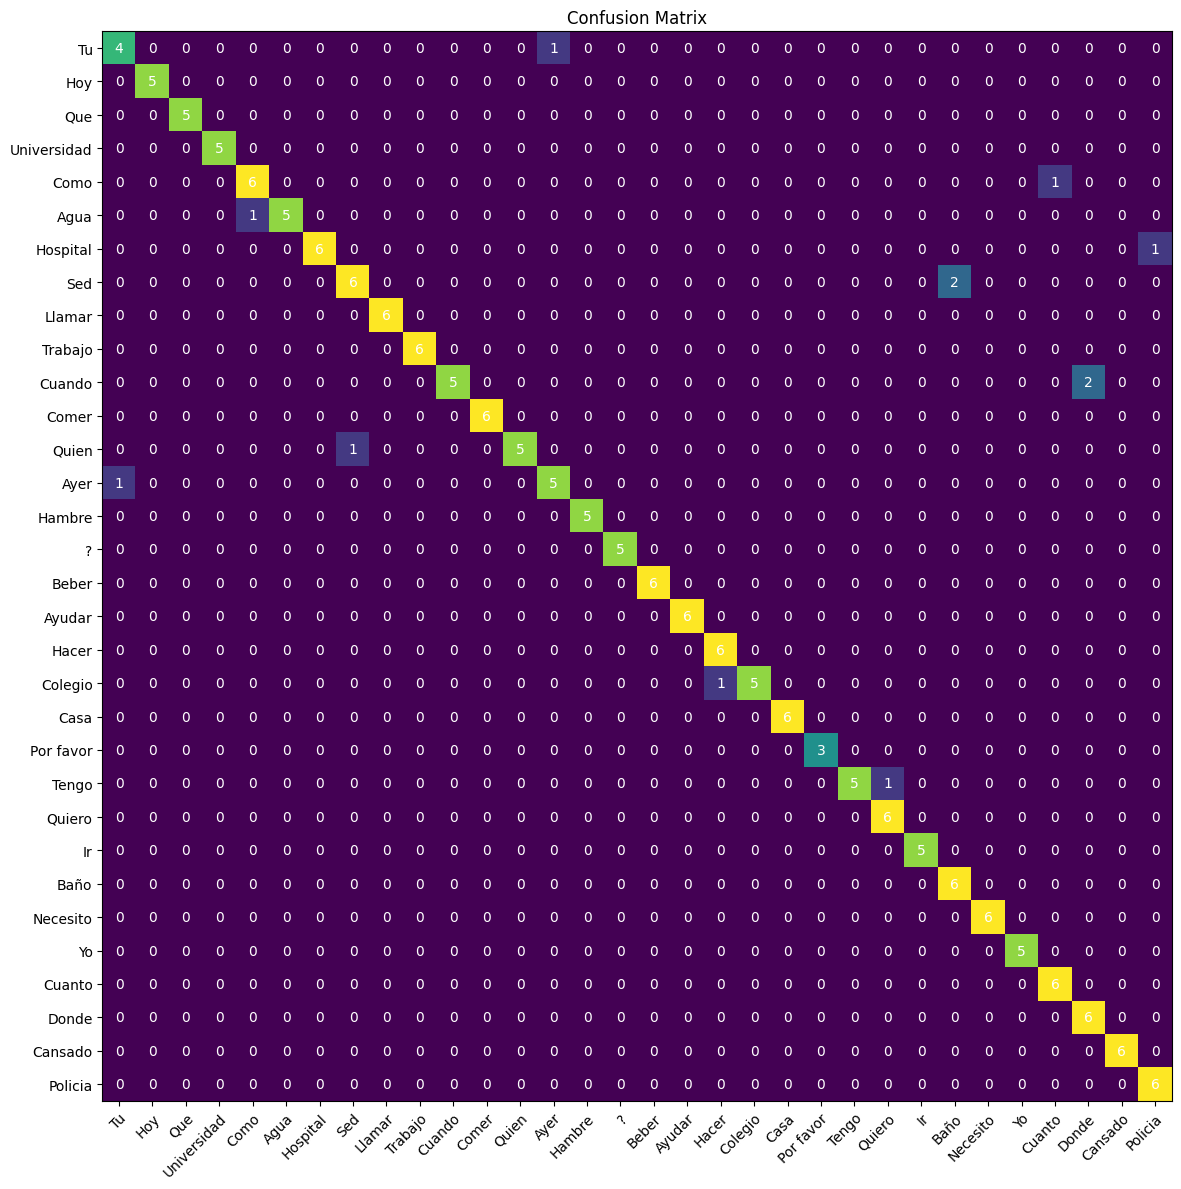
\includegraphics[width=0.7\textwidth]{figuras/modelDropoutBNCM.png}
    \caption{Matriz de confusión del primer model con dropout y normalización por lotes}
    \label{fig:CMModeloDropoutBN}
\end{figure}

La composición del segundo de los modelos se puede observar en la Figura \ref{fig:ModeloDropoutBNV2}.

\begin{figure}[H]
    \centering
    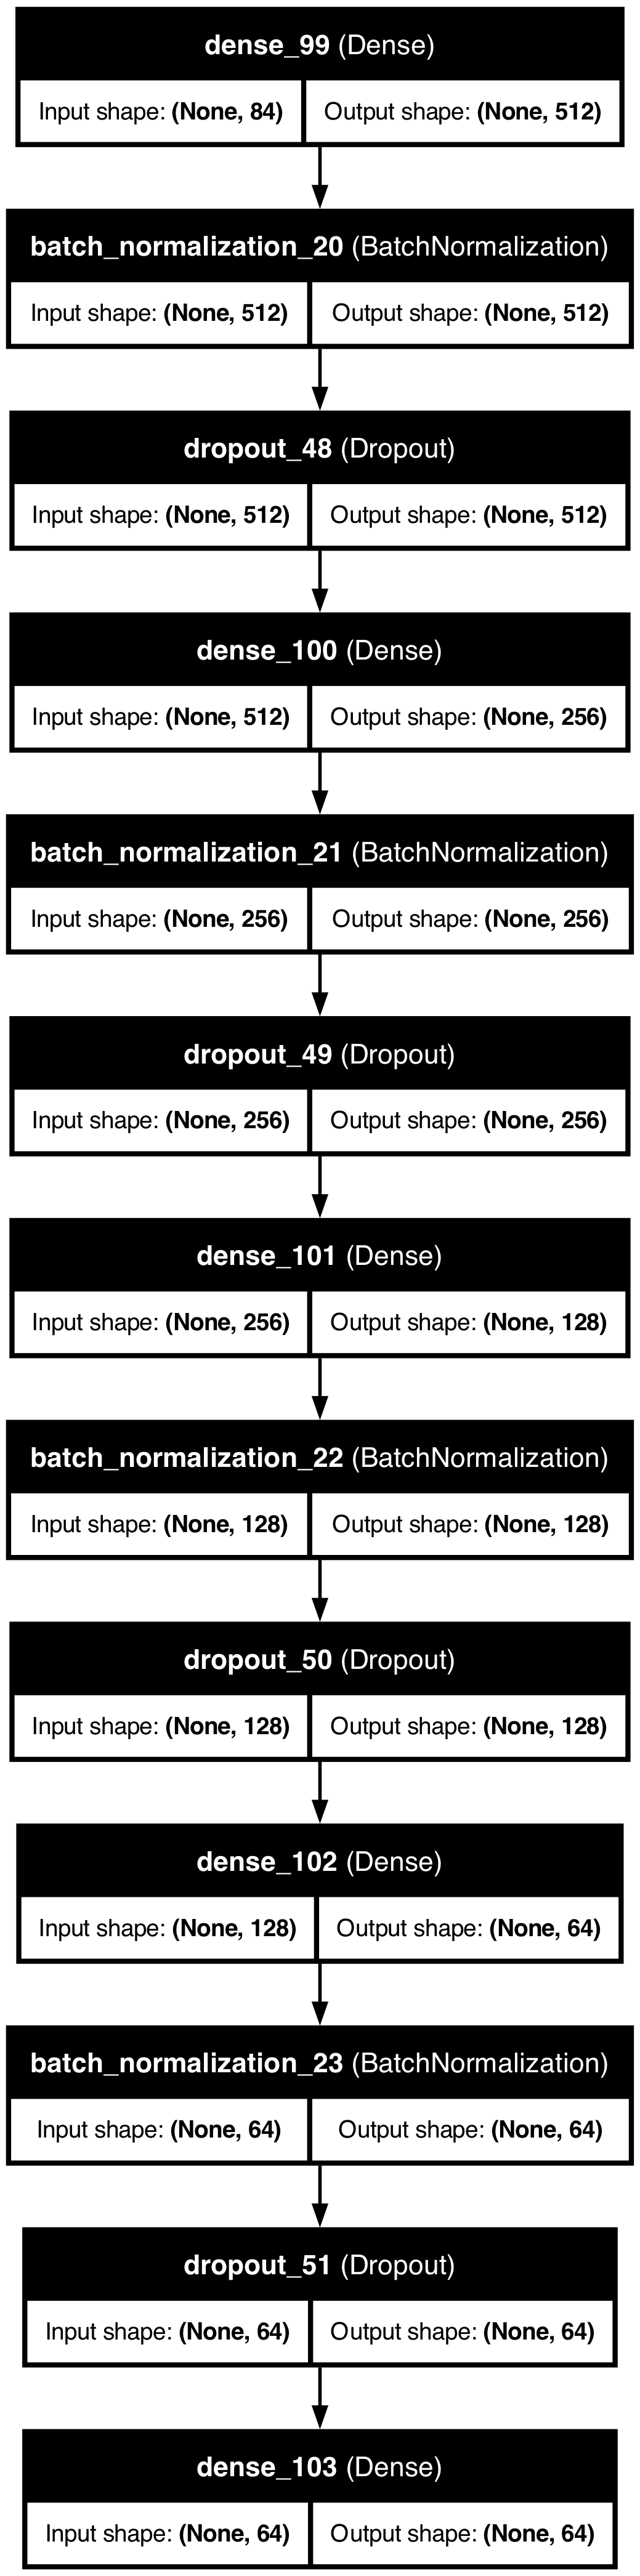
\includegraphics[width=0.345\textwidth]{figuras/modelDropoutBNV2.png}
    \caption{Segundo modelo con dropout y normalización por lotes}
    \label{fig:ModeloDropoutBNV2}
\end{figure}

El desempeño de este modelo se puede observar en la tabla \ref{tab:DesempeñoModeloDropoutBNV2}.
Este modelo tiene una precisión de 0.8593, una sensibilidad de 0.9461 y un F1 de 0.9441.
Adicional a esto, se puede observar la matriz de confusión en la Figura \ref{fig:CMModeloDropoutBNV2} y el historial de entrenamiento en la Figura \ref{fig:HistoryModeloDropoutBNV2}.

\begin{figure}[H]
    \centering
    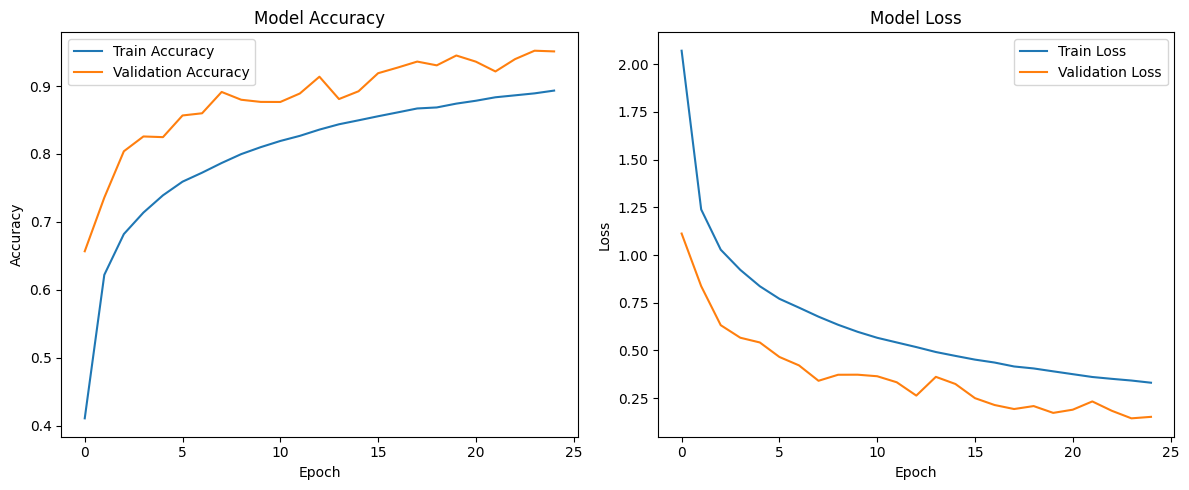
\includegraphics[width=0.7\textwidth]{figuras/modelDropoutBNV2History.png}
    \caption{Historial de entrenamiento del segundo modelo con dropout y normalización por lotes}
    \label{fig:HistoryModeloDropoutBNV2}
\end{figure}

\begin{table}[H]
    \centering
    \begin{tabular}{|c|c|}
        \hline
        \textbf{Métrica} & \textbf{Valor} \\
        \hline
        Precisión & 0.8802 \\
        \hline
        Sensibilidad & 0.9685 \\
        \hline
        F1 & 0.9706 \\
        \hline
    \end{tabular}
    \caption{Desempeño del segundo modelo con dropout y normalización por lotes}
    \label{tab:DesempeñoModeloDropoutBNV2}
\end{table}

\begin{figure}[H]
    \centering
    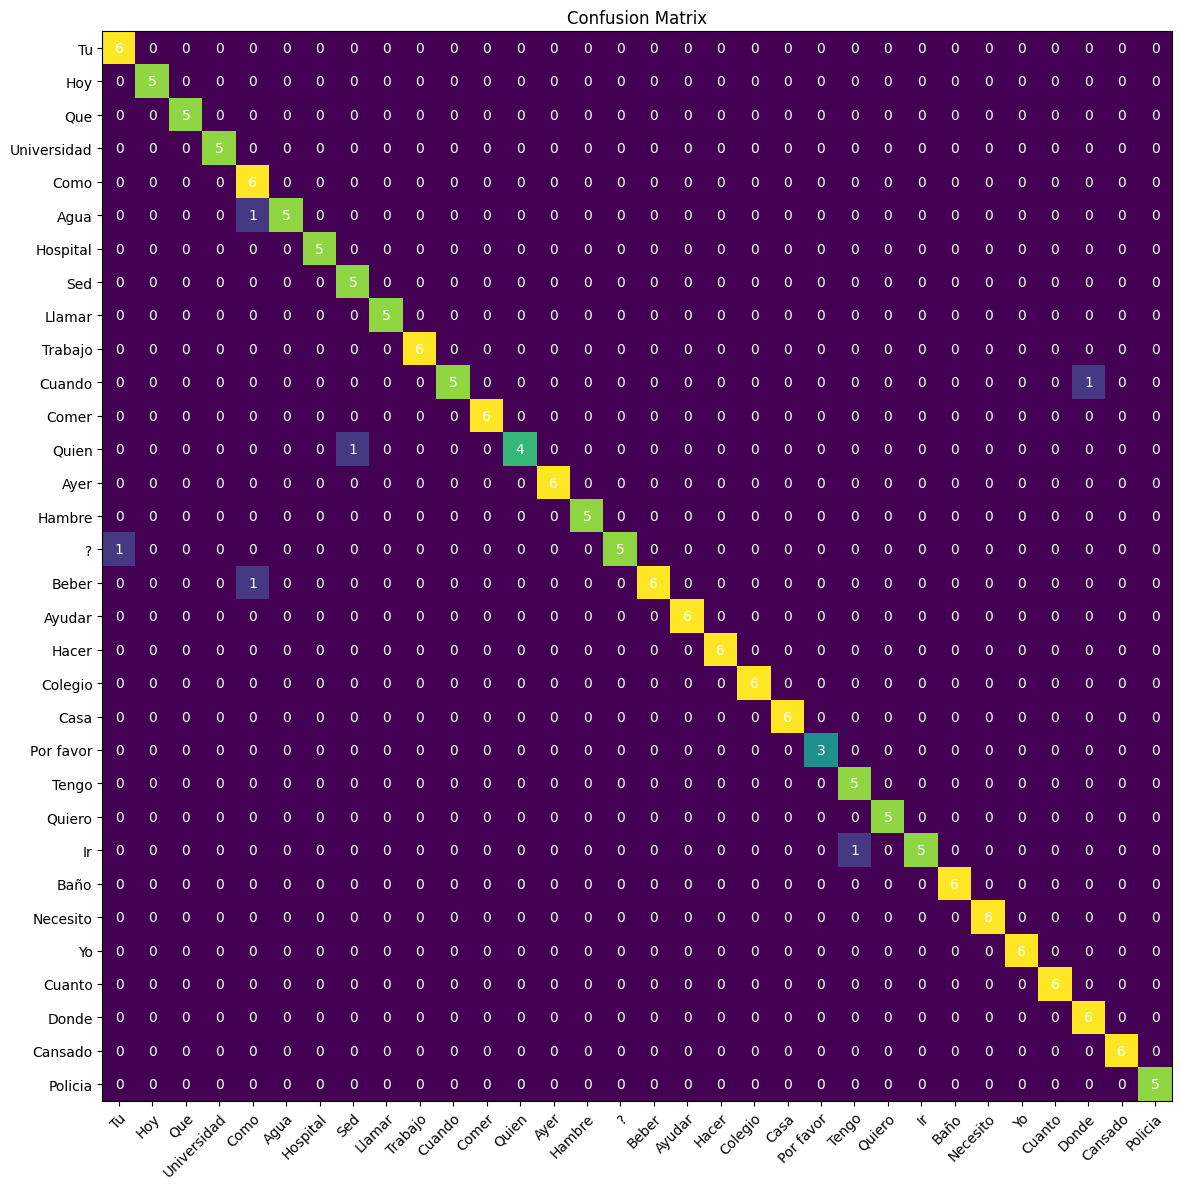
\includegraphics[width=0.7\textwidth]{figuras/modelDropoutBNV2CM.png}
    \caption{Matriz de confusión del segundo modelo con dropout y normalización por lotes}
    \label{fig:CMModeloDropoutBNV2}
\end{figure}

\subsubsection{Elección del modelo final}

El modelo final seleccionado es el modelo con dropout y normalización por lotes, con una precisión de 0.8802, una sensibilidad de 0.9685 y un F1 de 0.9706.
Este modelo tiene un desempeño superior a los modelos anteriores, lo cual indica que la combinación de dropout y normalización por lotes es efectiva para mejorar el desempeño del modelo.
Al observar la matriz de confusión en la Figura \ref{fig:CMModeloDropoutBNV2}, se puede observar que el modelo tiene un buen desempeño en la mayoría de las clases.

\subsection{Evaluación del modelo}

\subsubsection{Reconocimiento de una palabra}

El modelo final fue implementado en una aplicación de reconocimiento de lengua de señas de Guatemala en tiempo real, la cual se probó con un conjunto de datos de prueba.
Este conjunto de datos de prueba está compuesto de 192 videos, los cuales contienen gestos de 32 palabras de la lengua de señas de Guatemala.
Al utilizar el modelo final, se obtuvieron resultados satisfactorios, ya que el modelo fue capaz de reconocer correctamente los gestos de lengua de señas en tiempo real.
En la Figura \ref{fig:RealTimeRecognitionUnica} se puede observar el desempeño del modelo en tiempo real.
Adicionalmente, se puede observar el desempeño del modelo en la tabla \ref{tab:DesempeñoModeloFinal}.

\begin{table}[H]
    \centering
    \begin{tabular}{|c|c|}
        \hline
        \textbf{Métrica} & \textbf{Valor} \\
        \hline
        Precisión & 0.8802 \\
        \hline
        Sensibilidad & 0.9685 \\
        \hline
        F1 & 0.9706 \\
        \hline
        FPS promedio & 19.38 \\
        \hline
    \end{tabular}
    \caption{Desempeño del segundo modelo de la combinación de dropout y normalización por lotes}
    \label{tab:DesempeñoModeloFinal}
\end{table}

\begin{figure}[H]
    \centering
    \includegraphics[width=0.7\textwidth]{figuras/Resultados-1Seña.png}
    \caption{Reconocimiento de lengua de señas de Guatemala en tiempo real (una palabra)}
    \label{fig:RealTimeRecognitionUnica}
\end{figure}

\subsubsection{Reconocimiento de múltiples palabras}

Para evaluar el desempeño del modelo en la detección de múltiples palabras, se utilizó un conjunto de datos de prueba con videos de varias señas.
Este conjunto de datos de prueba está compuesto de 27 videos, los cuales contienen gestos de 2 a 4 palabras de la lengua de señas de Guatemala.
Al utilizar el modelo final, no se obtuvieron resultados satisfactorios, ya que el modelo no fue capaz de reconocer correctamente los gestos de lengua de señas en tiempo real.
En la Figura \ref{fig:RealTimeRecognition} se puede observar el desempeño del modelo en tiempo real.

\begin{figure}[H]
    \centering
    \includegraphics[width=0.8\textwidth]{figuras/Resultados-MultiSeñas.png}
    \caption{Reconocimiento de lengua de señas de Guatemala en tiempo real (múltiples palabras)}
    \label{fig:RealTimeRecognition}
\end{figure}

\subsection{Aplicaciones del modelo}

\subsubsection{Pruebas en tiempo real}

En las pruebas realizadas en tiempo real, el modelo final fue capaz de reconocer correctamente los gestos de lengua de señas de Guatemala en la mayoría de los casos.
Estas pruebas permitierón observar como el modelo se comporta en un entorno real, y si es capaz de reconocer todos los puntos clave de las señas.
A continuación se muestran algunas capturas de pantalla de la aplicación de reconocimiento de lengua de señas de Guatemala en tiempo real.
Cabe mencionar que cada uno de estos dos videos fueron grabados en diferentes angulos, con diferentes dispositivos, y con diferentes personas realizando los gestos.
Las figuras \ref{fig:RealTimeRecognition1}, y \ref{fig:RealTimeRecognition2} muestran el funcionamiento de la aplicación en tiempo real, con las palabras \textit{ayer} y \textit{comer}, respectivamente.

\begin{figure}[H]
    \centering
    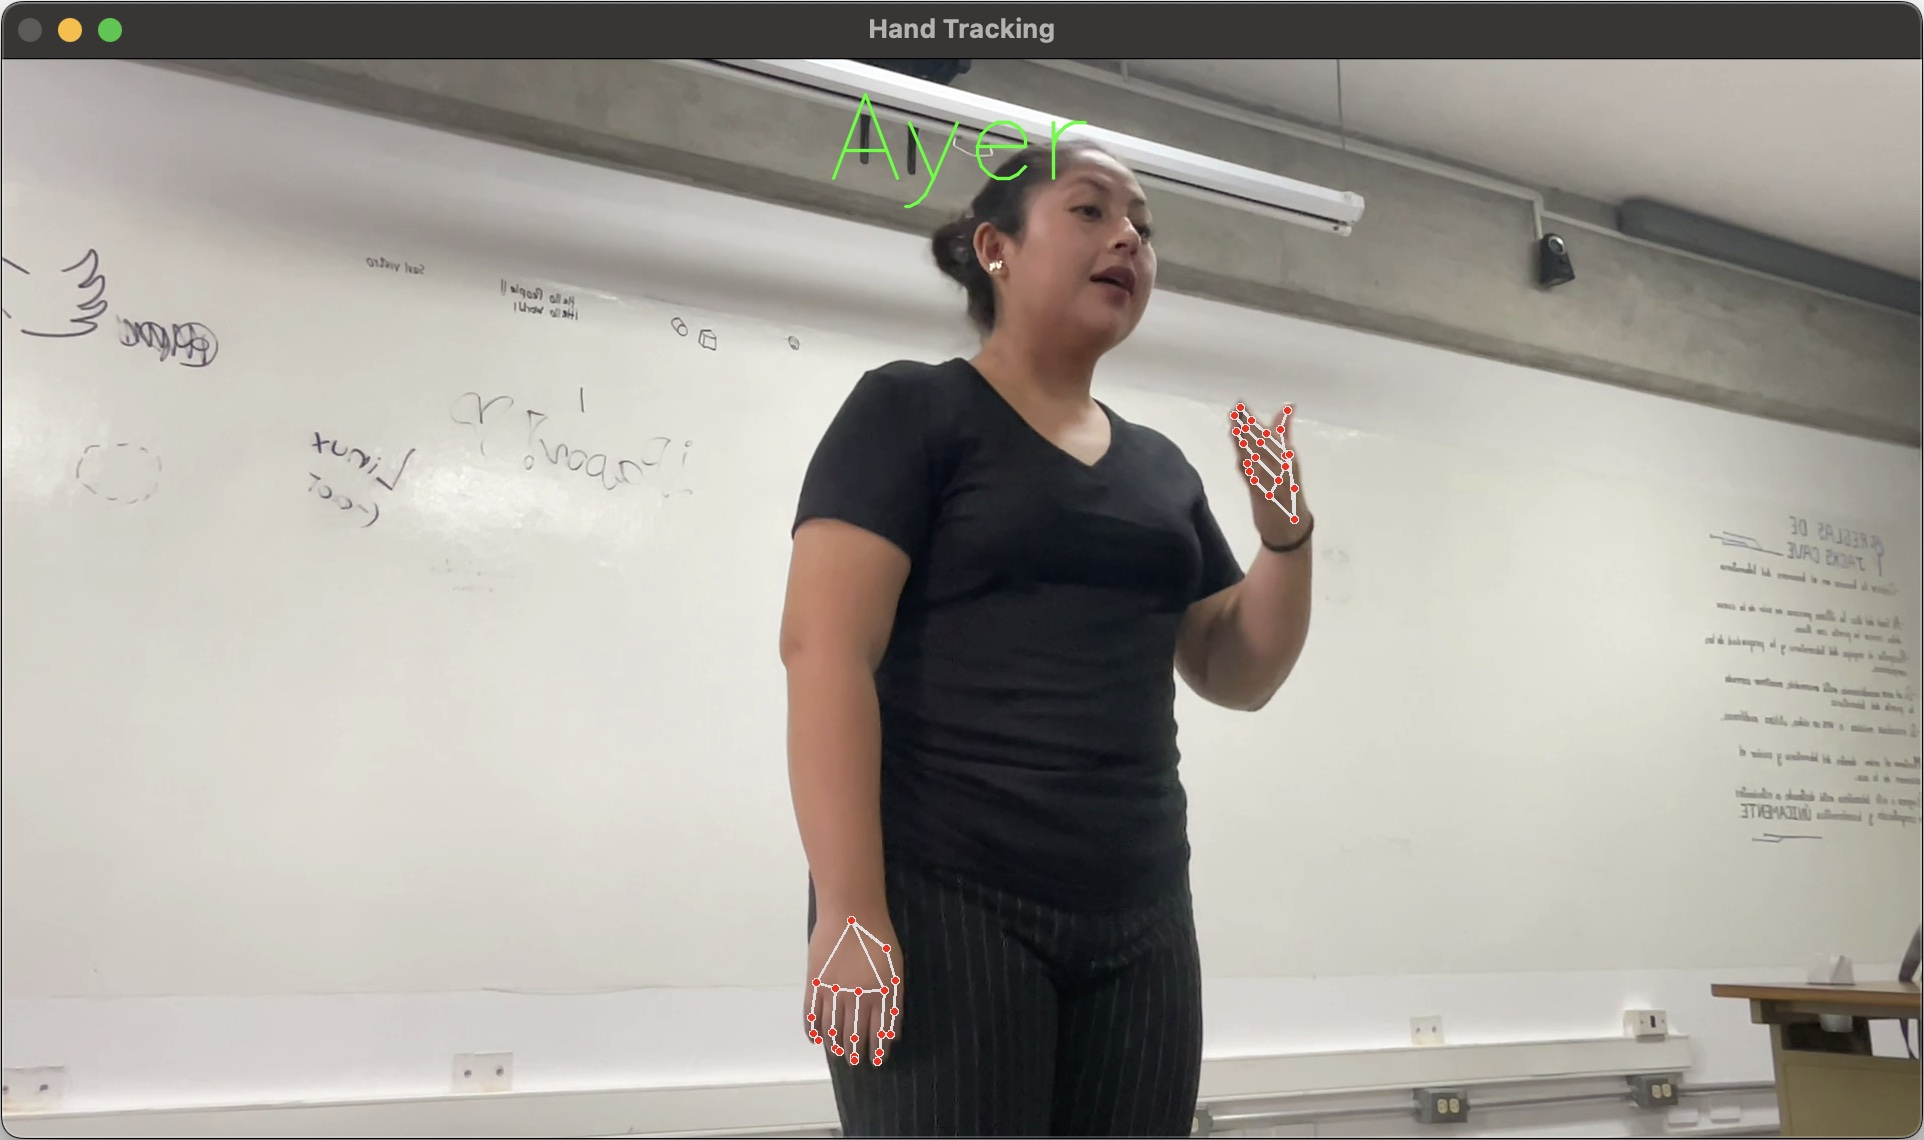
\includegraphics[width=0.9\textwidth]{figuras/PruebaDemo1.jpeg}
    \caption{Reconocimiento de la palabra \textit{ayer} en tiempo real}
    \label{fig:RealTimeRecognition1}
\end{figure}

\begin{figure}[H]
    \centering
    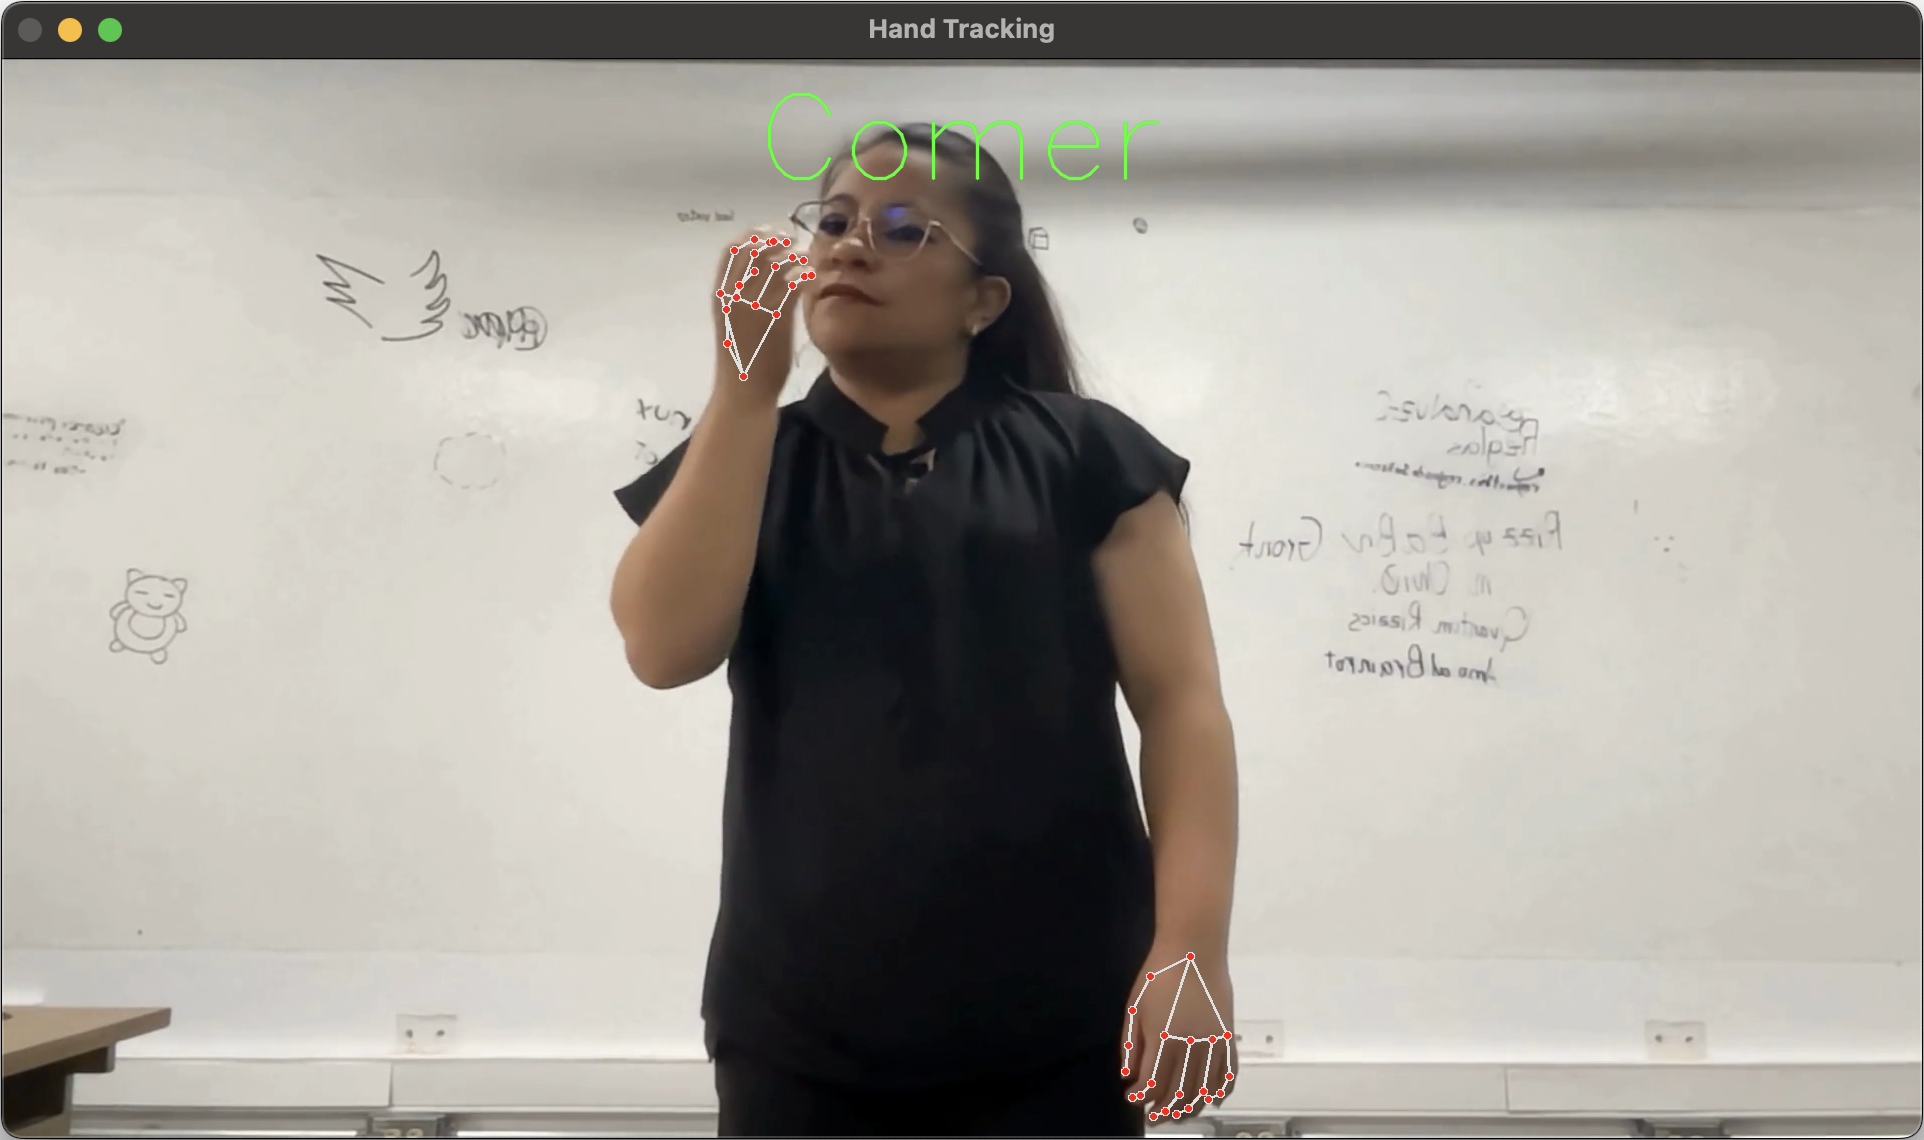
\includegraphics[width=0.9\textwidth]{figuras/PruebaDemo2.png}
    \caption{Reconocimiento de la palabra \textit{comer} en tiempo real}
    \label{fig:RealTimeRecognition2}
\end{figure}

\subsubsection{Pruebas del API}

El modelo final fue implementado en una Interfaz de Programación de Aplicaciones (API), la cual fue probada utilizando Postman y permitió acceder al modelo de reconocimiento de lengua de señas de forma remota.
A continuación se muestran algunas capturas de pantalla de las pruebas realizadas con el API.
Las figuras \ref{fig:APIRecognition1}, y \ref{fig:APIRecognition2} muestran el funcionamiento del API, con las palabras \textit{universidad} y \textit{tu}, respectivamente.

\begin{figure}[H]
    \centering
    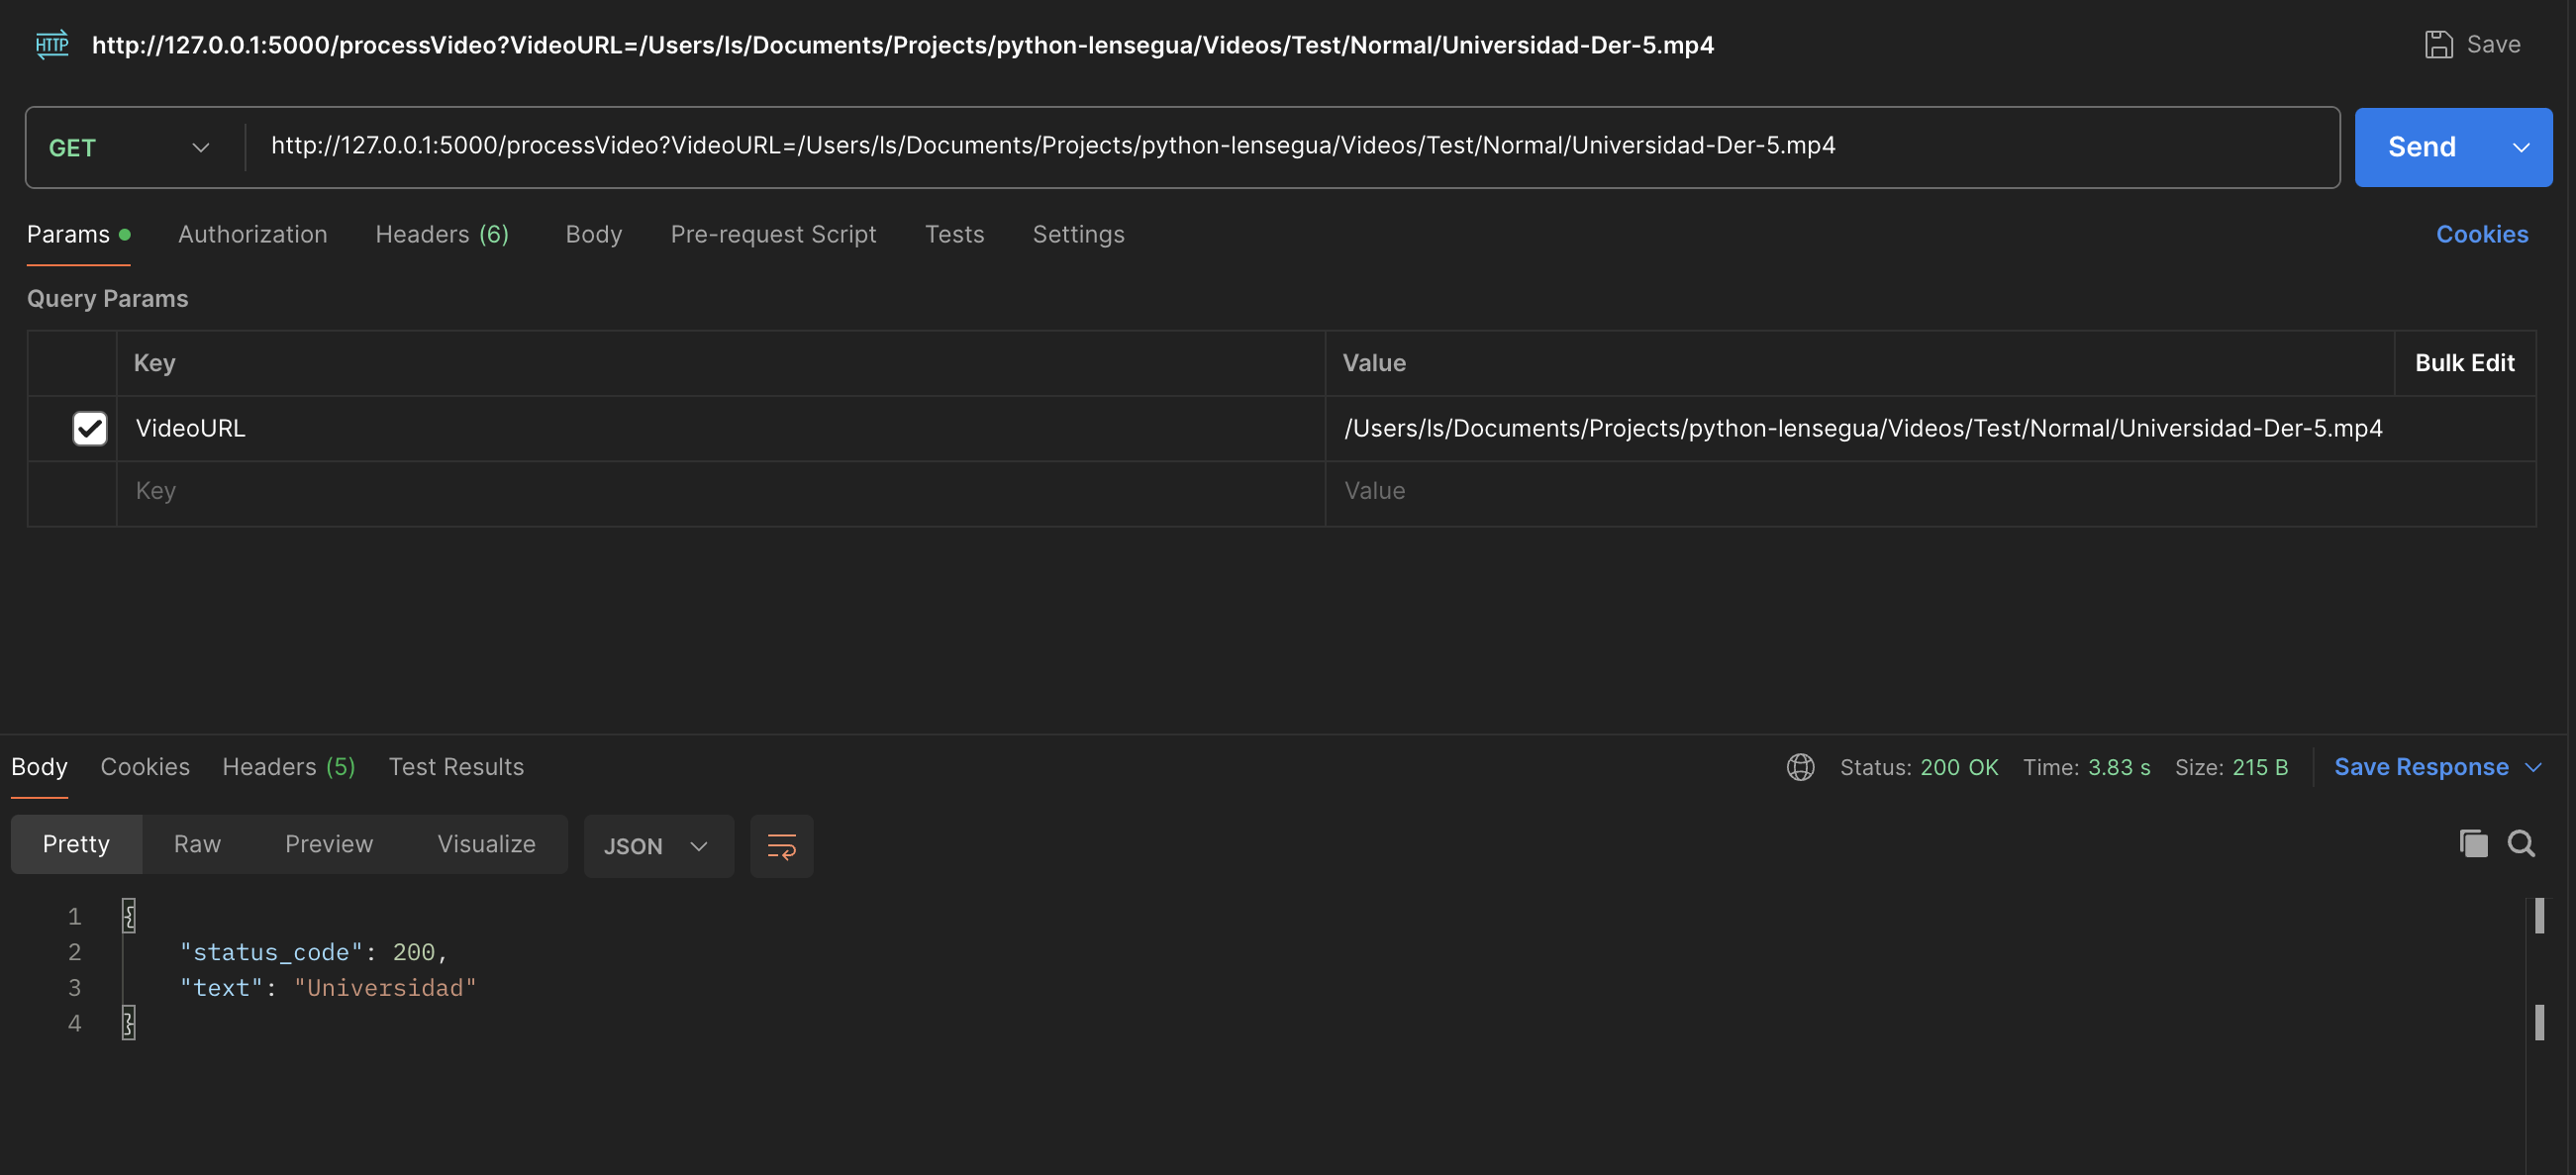
\includegraphics[width=0.9\textwidth]{figuras/PruebaAPI1.png}
    \caption{Reconocimiento de la palabra \textit{universidad} utilizando el API}
    \label{fig:APIRecognition1}
\end{figure}

\begin{figure}[H]
    \centering
    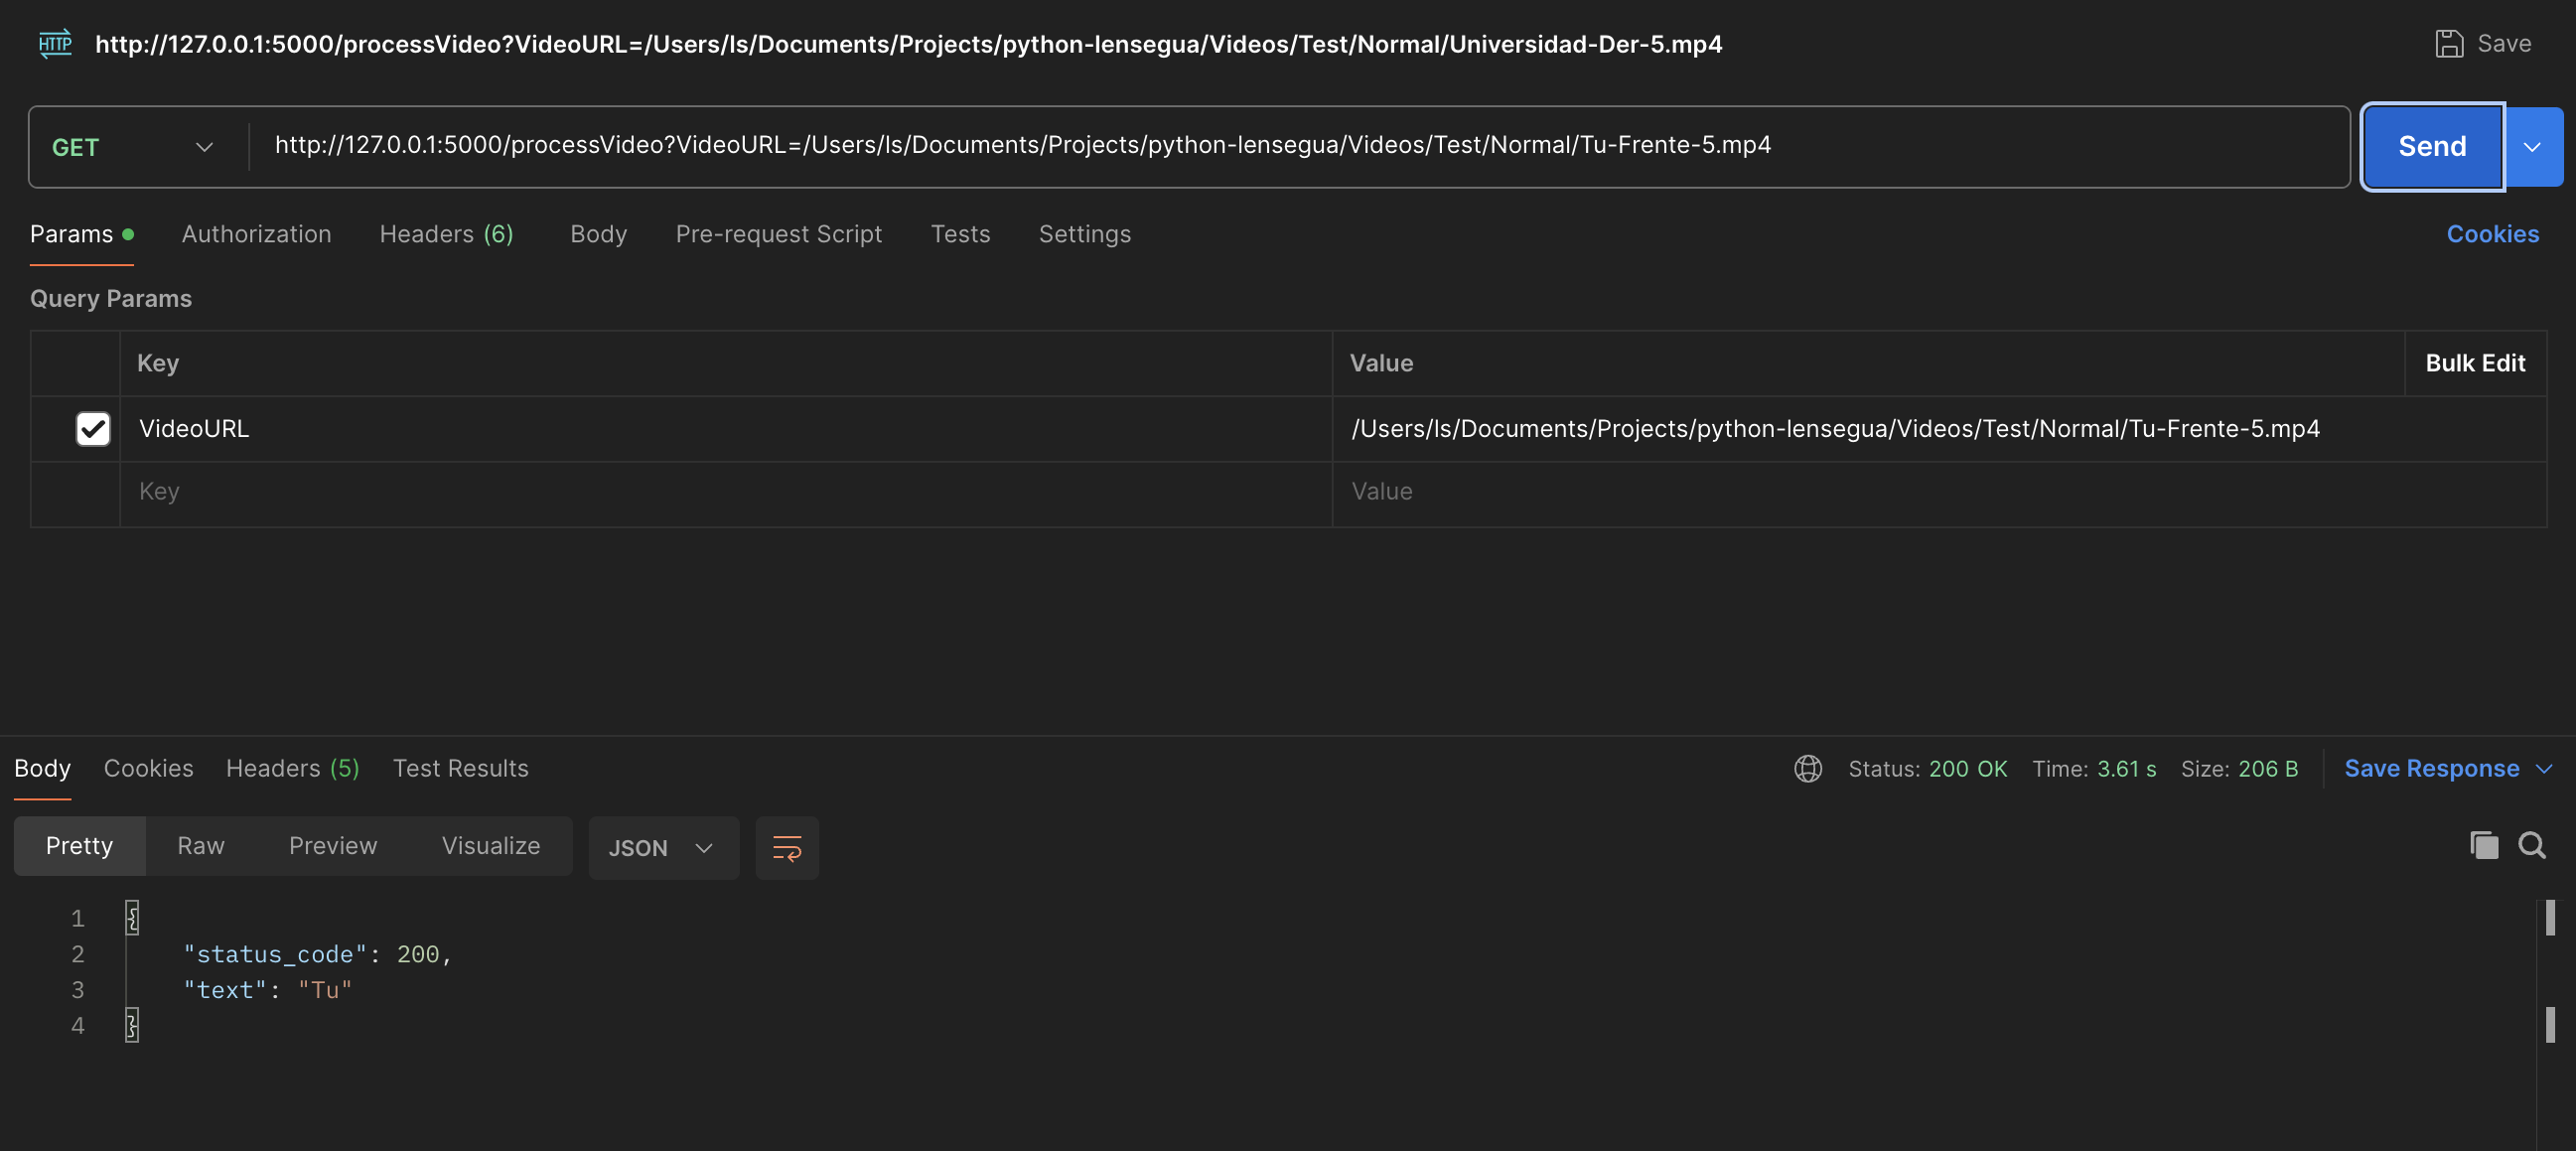
\includegraphics[width=0.9\textwidth]{figuras/PruebaAPI2.png}
    \caption{Reconocimiento de la palabra \textit{tu} utilizando el API}
    \label{fig:APIRecognition2}
\end{figure}




% Modulo de Chat
\section{Procesamiento de lenguaje natural (GPT-3.5-Turbo)} 

\subsection{Fine-tuning}

Antes de proceder con el \textit{fine-tuning} del modelo GPT-3.5-Turbo, se llevaron a cabo experimentos preliminares para identificar los parámetros que generaban la menor pérdida de validación. Esta métrica indica la eficacia del modelo para predecir correctamente las salidas a partir de las entradas proporcionadas. Una menor pérdida de validación sugiere que el modelo está aprendiendo de manera efectiva y puede generalizar mejor a datos no vistos. En la Tabla \ref{tab:hyperparam-tuning}, se presentan los valores de los parámetros ajustados durante estas pruebas, junto con la pérdida de validación correspondiente a cada configuración.

\vspace{0.5cm}
\begin{table}[H]
\centering
\begin{tabular}{|c|c|c|c|}
\hline
\textbf{Epochs} & \textbf{Batch Size} & \textbf{Learning Rate Multiplier} & \textbf{Pérdida de Validación} \\ \hline
2               & 16                  & 0.2                             & 0.1267                          \\ \hline
1               & 16                  & 0.3                            & 0.1334                          \\ \hline
1              & 8                  & 0.5                            & 0.2383                          \\ \hline
2              & 1                  & 2                             & 0.3163                          \\ \hline
3              & 1                  & 2                             & 0.4418                          \\ \hline
6              & 1                  & 2                             & 0.5966                          \\ \hline
\end{tabular}
\caption{Valores de parámetros y pérdidas de validación en experimentos preliminares}
\label{tab:hyperparam-tuning}
\end{table}

Tras analizar los resultados de estas pruebas, se decidió llevar a cabo el \textit{fine-tuning} final utilizando el conjunto de datos de entrenamiento completo y los parámetros que demostraron generar la menor pérdida de validación. Los parámetros seleccionados fueron: 2 \textit{epochs}, un \textit{batch size} de 16 y un \textit{learning rate multiplier} de 0.2.

\vspace{0.5cm}
\begin{table}[H]
\centering
\begin{tabular}{|l|c|}
\hline
\textbf{Parámetro} & \textbf{Valor} \\
\hline
Epochs & 2 \\
\hline
Batch size & 16 \\
\hline
Learning Rate Multiplier & 0.2 \\
\hline
\end{tabular}
\caption{Parámetros utilizados para el \textit{fine-tuning} del modelo GPT-3.5-Turbo.}
\label{tab:params-fine-tuning}
\end{table}

Durante el proceso de \textit{fine-tuning}, la plataforma de OpenAI generó una gráfica que se actualizaba con cada paso del entrenamiento, lo que facilitó el monitoreo de la evolución de la pérdida en tiempo real. La gráfica final, presentada en la Figura \ref{fig:LOSS}, confirmó que el modelo no presentaba signos de \textit{overfitting}, es decir que el modelo resultante tenía la capacidad para adaptarse a nuevos datos. Esta observación fue fundamental para garantizar que el modelo pudiera aplicarse efectivamente en situaciones prácticas.

\begin{figure}[H]
\centering
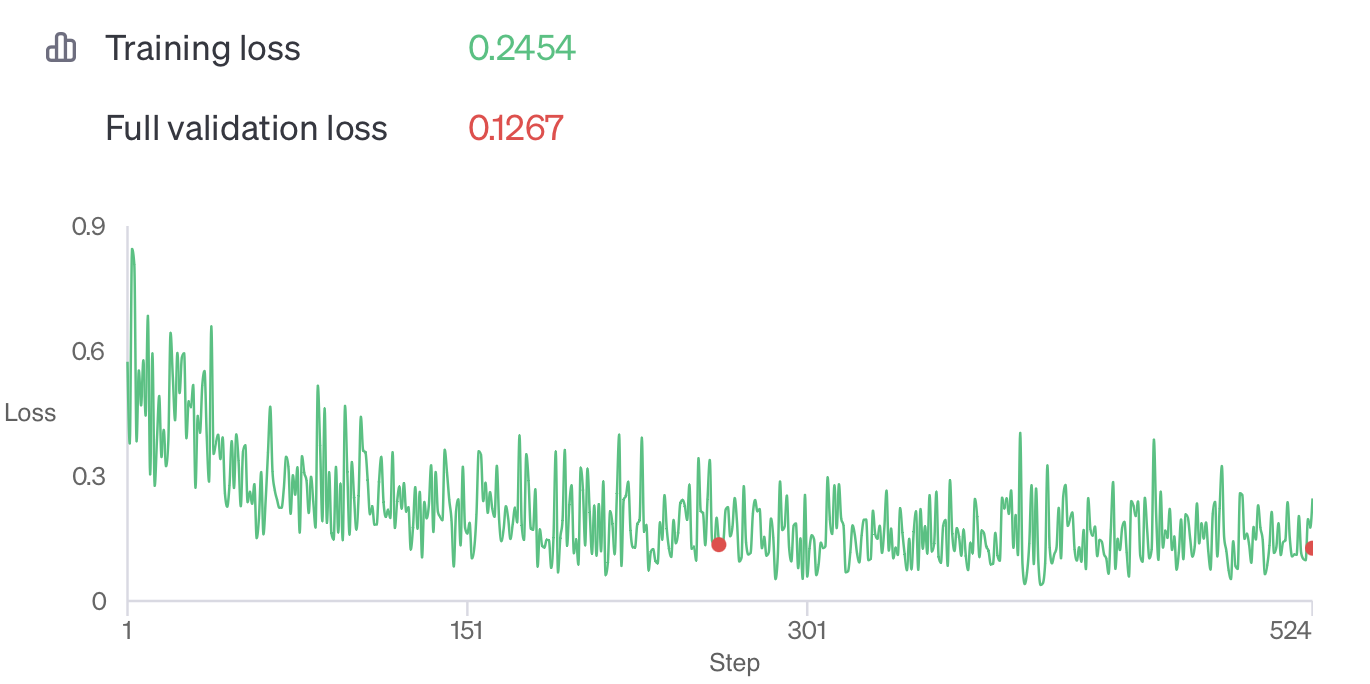
\includegraphics[width=0.75\linewidth]{figuras/LOSS.png}
\caption{Evolución de la pérdida durante el \textit{fine-tuning} final del modelo GPT-3.5-Turbo.}
\label{fig:LOSS}
\end{figure}

Una vez completado el \textit{fine-tuning} del modelo GPT-3.5-Turbo, se utilizó la técnica de \textit{Local Interpretable Model-agnostic Explanations} (LIME) para evaluar el impacto de este proceso en las interpretaciones generadas por el modelo. LIME permitió identificar, para frases específicas, qué palabras influían más en las respuestas de ambos modelos, facilitando el análisis de cómo cada uno priorizaba ciertos elementos del texto al generar sus respuestas. Para ello, se seleccionaron tres frases representativas de la gramática de LENSEGUA, diseñadas para evaluar la capacidad de los modelos en interpretar estructuras lingüísticas clave, como marcadores temporales, términos interrogativos y otras palabras funcionales.

Las Figuras \ref{fig:LIME-O1} y \ref{fig:LIME-F1} presentan los resultados de los análisis LIME realizados para la frase “antes tu policía llamar pregunta”. Cada visualización proporciona información detallada sobre el impacto de cada palabra en las respuestas generadas por ambos modelos, codificándolas por colores y asociándolas a un valor numérico específico. En ambas figuras, las palabras resaltadas en azul (con valores cercanos a -1) fueron aquellas que generaron confusión, resultando en respuestas menos alineadas con la interpretación teórica establecida. En contraste, las palabras resaltadas en naranja (con valores cercanos a 1) contribuyeron de manera positiva, ayudando a formular interpretaciones más precisas.

Estos resultados se resumen en la Tabla \ref{tab:LIME-1}, donde destaca un cambio significativo en la palabra “pregunta”, que pasó de tener una influencia negativa (-0.09) en el modelo estándar a una positiva (0.09) en el modelo adaptado. Esta transformación sugiere que el \textit{fine-tuning} mejoró la capacidad del modelo para reconocer y procesar marcadores interrogativos. Adicionalmente, las palabras “policía” y “llamar” también mostraron un aumento en su relevancia en el modelo adaptado (0.43 y 0.20, respectivamente), en comparación con el modelo estándar (0.13 y 0.07). 

\begin{figure}[H]
\centering
    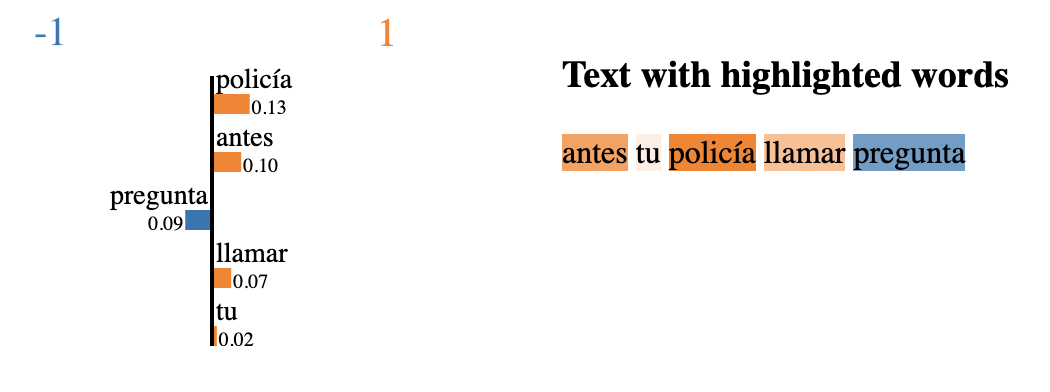
\includegraphics[width=0.7\textwidth]{figuras/LIME/LIME-O1.png}
    \caption{Resultados de LIME para la interpretación generada por el modelo GPT-3.5-Turbo estándar para la frase “antes tu policía llamar pregunta”.}
    \label{fig:LIME-O1}
\end{figure}

\begin{figure}[H]
\centering
    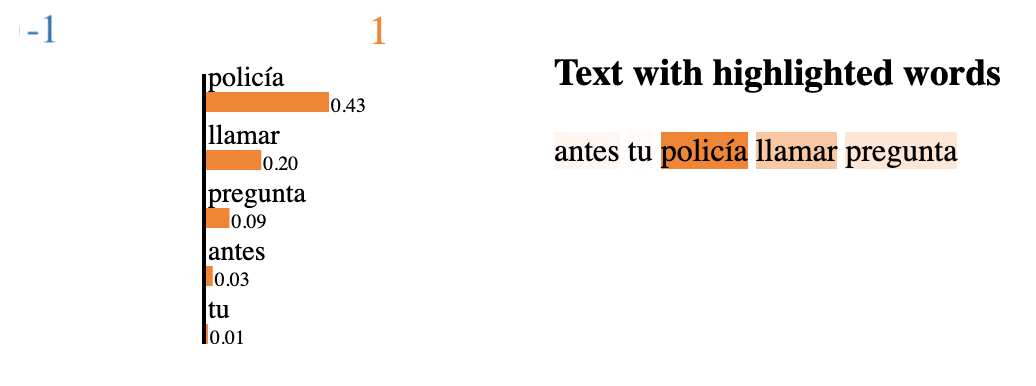
\includegraphics[width=0.7\textwidth]{figuras/LIME/LIME-F1.png}
    \caption{Resultados de LIME para la interpretación generada por el modelo GPT-3.5-Turbo \textit{fine-tuneado} para la frase “antes tu policía llamar pregunta”.}
    \label{fig:LIME-F1}
\end{figure}

\vspace{0.5cm}
\begin{table}[H]
\centering
    \begin{tabular}{|l|c|c|}
        \hline
        \multicolumn{3}{|l|}{\textbf{Frase en LENSEGUA:} antes tu policía llamar pregunta} \\ \hline
        \multicolumn{3}{|l|}{\textbf{Interpretación teórica:} ¿Llamaste a la policía?} \\ \hline \hline
        
        \textbf{Palabra} & \multicolumn{2}{c|}{\textbf{Valores de Influencia (LIME)}} \\ 
        \cline{2-3}
         & \textbf{Modelo GPT-3.5-Turbo} & \textbf{Modelo \textit{fine-tuneado}} \\
         
        \hline
        antes & 0.10 & 0.03 \\
        \hline
        tu & 0.02 & 0.01 \\
        \hline
        policía & 0.13  & 0.43 \\
        \hline
        llamar & 0.07  & 0.20 \\
        \hline
        pregunta & -0.09  & 0.09 \\
        \hline
    \end{tabular}
\caption{Contribución de cada palabra según los Valores de Influencia (LIME) en las interpretaciones generadas por el modelo GPT-3.5-Turbo estándar y su versión \textit{fine-tuneada} para la frase “antes tu policía llamar pregunta”.}
\label{tab:LIME-1}
\end{table}

En la Tabla \ref{tab:LIME-2} se presentan los resultados para la frase “futuro hospital él ir”. El marcador temporal “futuro” mostró el cambio más significativo, pasando de una influencia negativa de -0.04 en el modelo estándar (ver Figura \ref{fig:LIME-O2}) a una positiva de 0.09 en el modelo adaptado (ver Figura \ref{fig:LIME-F2}). Esto indica que el modelo ajustado reconoció mejor la importancia de “futuro” como un elemento clave para la interpretación de la frase. Por otro lado, la palabra “hospital” aumentó su relevancia (de 0.34 a 0.51), mientras que las influencias de “él” e “ir” experimentaron una ligera reducción.

\begin{figure}[H]
\centering
    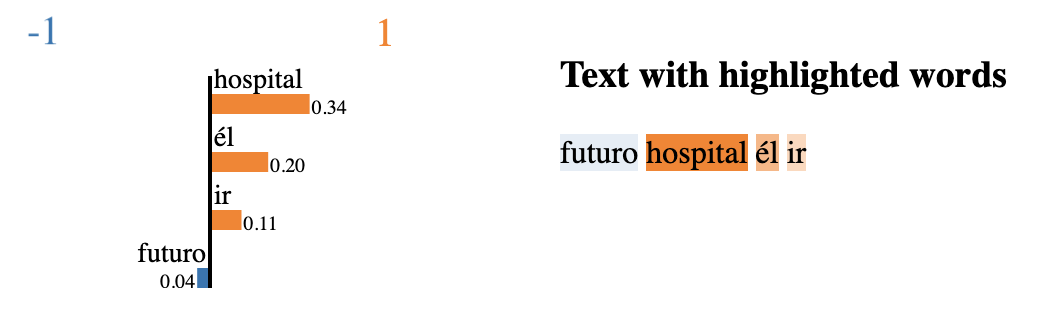
\includegraphics[width=0.7\textwidth]{figuras/LIME/LIME-O2.png}
    \caption{Resultados de LIME para la interpretación generada por el modelo GPT-3.5-Turbo estándar para la frase “futuro hospital él ir”.}
    \label{fig:LIME-O2}
\end{figure}

\begin{figure}[H]
\centering
    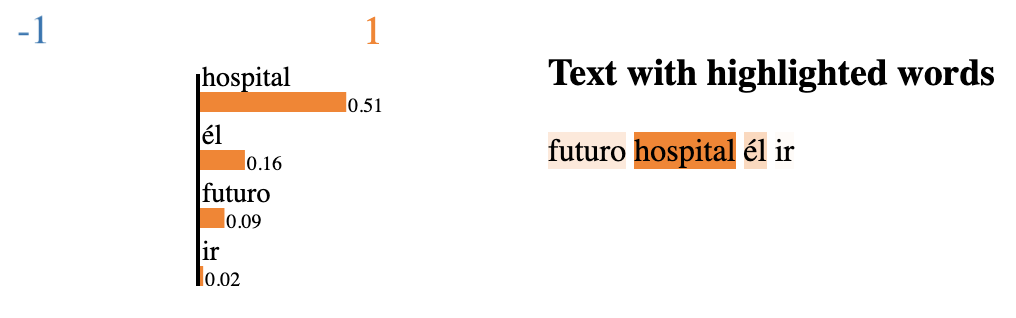
\includegraphics[width=0.7\textwidth]{figuras/LIME/LIME-F2.png}
    \caption{Resultados de LIME para la interpretación generada por el modelo GPT-3.5-Turbo \textit{fine-tuneado} para la frase “futuro hospital él ir”.}
    \label{fig:LIME-F2}
\end{figure}

\vspace{0.5cm}
\begin{table}[H]
\centering
    \begin{tabular}{|l|c|c|}
        \hline
        \multicolumn{3}{|l|}{\textbf{Frase en LENSEGUA:} futuro hospital él ir} \\ \hline
        \multicolumn{3}{|l|}{\textbf{Interpretación teórica:} Él irá al hospital.} \\ \hline \hline
        
        \textbf{Palabra} & \multicolumn{2}{c|}{\textbf{Valores de Influencia (LIME)}} \\ 
        \cline{2-3}
         & \textbf{Modelo GPT-3.5-Turbo} & \textbf{Modelo \textit{fine-tuneado}} \\
         
        \hline
        futuro & -0.04 & 0.09 \\
        \hline
        hospital & 0.34 & 0.51 \\
        \hline
        él & 0.20  & 0.16 \\
        \hline
        ir & 0.11  & 0.02 \\
        \hline
        
    \end{tabular}
\caption{Contribución de cada palabra según los Valores de Influencia (LIME) en las interpretaciones generadas por el modelo GPT-3.5-Turbo estándar y su versión \textit{fine-tuneada} para la frase “futuro hospital él ir”.}
\label{tab:LIME-2}
\end{table}

La Tabla \ref{tab:LIME-3} muestra los resultados de los análisis LIME para la frase “pasado yo ir no”, combinando la información de las Figuras \ref{fig:LIME-O3} y \ref{fig:LIME-F3}. En este caso, se destaca un aumento significativo en el impacto del término “pasado”, que subió de 0.08 en el modelo estándar a 0.24 en el modelo \textit{fine-tuneado}. Además, la palabra “no” mostró un notable incremento en su relevancia, pasando de 0.12 a 0.44. Finalmente, la influencia de “ir” se redujo de 0.37 a 0.17, mientras que “yo” mostró una leve mejora, pasando de -0.03 a 0.06.

\begin{figure}[H]
\centering
    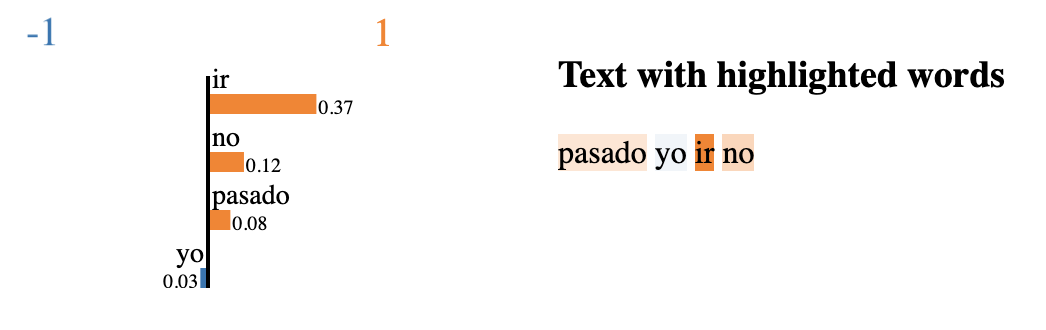
\includegraphics[width=0.7\textwidth]{figuras/LIME/LIME-O3.png}
    \caption{Resultados de LIME para la interpretación generada por el modelo GPT-3.5-Turbo estándar para la frase “pasado yo ir no”.}
    \label{fig:LIME-O3}
\end{figure}

\begin{figure}[H]
\centering
    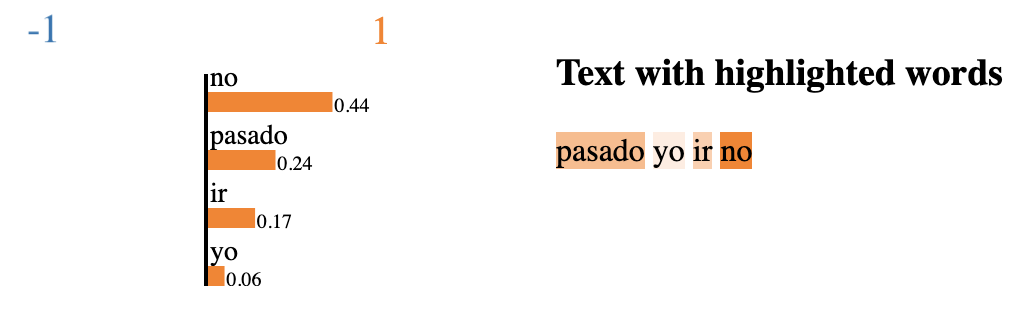
\includegraphics[width=0.7\textwidth]{figuras/LIME/LIME-F3.png}
    \caption{Resultados de LIME para la interpretación generada por el modelo GPT-3.5-Turbo \textit{fine-tuneado} para la frase “pasado yo ir no”.}
    \label{fig:LIME-F3}
\end{figure}

\vspace{0.5cm}
\begin{table}[H]
\centering
    \begin{tabular}{|l|c|c|}
        \hline
        \multicolumn{3}{|l|}{\textbf{Frase en LENSEGUA:} pasado yo ir no} \\ \hline
        \multicolumn{3}{|l|}{\textbf{Interpretación teórica:} No fui.} \\ \hline \hline
        
        \textbf{Palabra} & \multicolumn{2}{c|}{\textbf{Valores de Influencia (LIME)}} \\ 
        \cline{2-3}
         & \textbf{Modelo GPT-3.5-Turbo} & \textbf{Modelo \textit{fine-tuneado}} \\
         
        \hline
        pasado & 0.08 & 0.24 \\
        \hline
        yo & -0.03 & 0.06 \\
        \hline
        ir & 0.37  & 0.17 \\
        \hline
        no & 0.12  & 0.44 \\
        \hline
        
    \end{tabular}
\caption{Contribución de cada palabra según los Valores de Influencia (LIME) en las interpretaciones generadas por el modelo GPT-3.5-Turbo estándar y su versión \textit{fine-tuneada} para la frase “pasado yo ir no”.}
\label{tab:LIME-3}
\end{table}



\subsection{Prompt engineering}

Durante las fases iniciales, se utilizó el siguiente \textit{prompt} para guiar al modelo \textit{fine-tuneado} en la generación de interpretaciones. Este \textit{prompt} establecía las instrucciones necesarias para que el modelo actuara como un intérprete en LENSEGUA. Sin embargo, durante las pruebas realizadas, se identificaron varios aspectos que limitaron la calidad de las respuestas. En particular, se presentaron dificultades al procesar expresiones temporales, lo que resultó en errores y redundancias.

\vspace{0.5cm}
\begin{tcolorbox}[colback=gray!10, colframe=black, title=Prompt (versión 1)]
\textit{Eres un intérprete experto en Lengua de Señas de Guatemala (LENSEGUA). El usuario te proporcionará frases en español escritas utilizando la gramática de LENSEGUA. Tu tarea es interpretarlas y convertirlas en español gramaticalmente correcto.}
\end{tcolorbox}
\vspace{0.5cm}

Con el objetivo de mejorar la calidad de las interpretaciones, se llevó a cabo una fase de \textit{prompt engineering}. En esta etapa, se realizaron ajustes iterativos sobre el \textit{prompt} original, incorporando instrucciones más precisas para corregir errores recurrentes. Además, para evaluar la efectividad de cada variante, como se mencionó en la sección de metodología, se calculó la distancia de Levenshtein promedio utilizando el conjunto de validación, el modelo \textit{fine-tuneado} y las diferentes versiones de \textit{prompts}. En este contexto, se propuso un segundo \textit{prompt}.

\vspace{0.5cm}
\begin{tcolorbox}[colback=gray!10, colframe=black, title=Prompt (versión 2)] 
\textit{Soy un intérprete experto en Lengua de Señas de Guatemala (LENSEGUA). El usuario me proporcionará frases en español escritas utilizando la gramática de LENSEGUA. Mi tarea es interpretarlas y convertirlas en español gramaticalmente correcto.} \end{tcolorbox}
\vspace{0.5cm}

Para esta segunda versión, se decidió formular las instrucciones en primera persona en lugar de tercera. Esto se hizo para que el modelo asumiera un rol más activo en el proceso de interpretación. Sin embargo, a pesar de este cambio, la distancia de Levenshtein promedio obtenida con las interpretaciones generadas por el modelo \textit{fine-tuneado} y este nuevo \textit{prompt} fue de 5.84, ligeramente superior al valor de 5.815 obtenido con la primera versión. Además, tras una revisión de las interpretaciones, se identificó que los errores anteriormente mencionados aún persistían. Ante esto, se retomó el \textit{prompt} original y se elaboró una tercera versión del \textit{prompt} que especificaba claramente la exclusión de ciertos términos.

\vspace{0.5cm}
\begin{tcolorbox}[colback=gray!10, colframe=black, title=Prompt (versión 3)] 
\textit{Eres un intérprete experto en Lengua de Señas de Guatemala (LENSEGUA). El usuario te proporcionará frases en español escritas utilizando la gramática de LENSEGUA. Tu tarea es interpretarlas y convertirlas en español gramaticalmente correcto, teniendo en cuenta la siguiente regla específica:} 
\begin{itemize} 
    \item \textit{Las palabras “pasado”, “futuro” y “antes” indican la conjugación verbal. Debes conjugar correctamente los verbos en tu respuesta sin incluir las palabras “pasado”, “futuro” o “antes”.} 
\end{itemize} 
\end{tcolorbox}
\vspace{0.5cm}

Esta tercera versión mostró una mejora, con una distancia de Levenshtein promedio de 5.37. No obstante, se identificaron problemas en la interpretación de expresiones comunes en LENSEGUA que no tienen un equivalente directo en español. Aunque el modelo \textit{fine-tuneado} había sido expuesto a expresiones como ‘carro mucho’ (interpretado correctamente como ‘tráfico’) y ‘bien mucho’ (como ‘muy bien’) durante su entrenamiento, las respuestas que generaba eran inconsistentes; como si en ocasiones el modelo “olvidara” estas interpretaciones o no las aplicara de manera uniforme. Para asegurar respuestas más coherentes, se realizaron ajustes adicionales en el \textit{prompt}, añadiendo recordatorios específicos sobre cómo manejar dichas expresiones. Además, se incluyó una instrucción que prevenía al modelo de interpretar frases como preguntas, a menos que incluyeran términos como ‘pregunta’ o ‘si o no’. Estos cambios contribuyeron significativamente a mejorar la estabilidad y la precisión en las respuestas del modelo.

\vspace{0.5cm}
\begin{tcolorbox}[colback=gray!10, colframe=black, title=Prompt (versión 4)] 
\textit{Eres un intérprete experto en Lengua de Señas de Guatemala (LENSEGUA). El usuario te proporcionará frases en español escritas utilizando la gramática de LENSEGUA. Tu tarea es interpretarlas y convertirlas en español gramaticalmente correcto, teniendo en cuenta las siguientes reglas específicas:} 
\begin{itemize} 
    \item \textit{No debes interpretar las frases como preguntas, ni agregar una entonación interrogativa, a menos que incluyan las palabras “pregunta” o “sí o no”.} 
    \item \textit{Las palabras “pasado”, “futuro” y “antes” indican la conjugación verbal. Debes conjugar correctamente los verbos en tu respuesta sin incluir las palabras “pasado”, “futuro” o “antes”.} 
    \item \textit{La frase “carro mucho” debe interpretarse como “tráfico”.} 
    \item \textit{La frase “bien mucho” debe interpretarse como “muy bien”.} 
\end{itemize} 
\end{tcolorbox}
\vspace{0.5cm}

La cuarta versión del \textit{prompt} alcanzó una distancia de Levenshtein promedio de 4.30, calculada a partir de las interpretaciones generadas por el modelo \textit{fine-tuneado}. Al analizar detenidamente las interpretaciones individuales, se observó que la mayoría eran correctas. Sin embargo, en algunos casos, el modelo alteraba el orden de los elementos dentro de las oraciones, lo que, en comparación con lo esperado, afectaba negativamente la métrica de desempeño. Para intentar solventar esta situación, se incorporó una instrucción adicional que enfatizaba la necesidad de mantener una estructura y secuencia especifica en las interpretaciones finales.

\vspace{0.5cm}
\begin{tcolorbox}[colback=gray!10, colframe=black, title=Prompt (versión 5)] 
\textit{Eres un intérprete experto en Lengua de Señas de Guatemala (LENSEGUA). El usuario te proporcionará frases en español escritas utilizando la gramática de LENSEGUA. Tu tarea es interpretarlas y convertirlas en español gramaticalmente correcto, teniendo en cuenta las siguientes reglas específicas:} 
\begin{itemize} 
    \item \textit{No debes interpretar las frases como preguntas, ni agregar una entonación interrogativa, a menos que incluyan las palabras “pregunta” o “sí o no”.} 
    \item \textit{Las palabras “pasado”, “futuro” y “antes” indican la conjugación verbal. Debes conjugar correctamente los verbos en tu respuesta sin incluir las palabras “pasado”, “futuro” o “antes”.} 
    \item \textit{La frase “carro mucho” debe interpretarse como “tráfico”.} 
    \item \textit{La frase “bien mucho” debe interpretarse como “muy bien”.} 
    \item \textit{Mantén el orden de los elementos de la interpretación final lo más similar posible al texto original cuando sea gramaticalmente válido en español. Por ejemplo, si la frase en LENSEGUA es “Por favor cuando tu salir luz apagar”, la interpretación debe ser “Por favor cuando salgas apaga la luz” en lugar de “Por favor apaga la luz cuando salgas”.}
\end{itemize} 
\end{tcolorbox}
\vspace{0.5cm}

Esta última versión del \textit{prompt} obtuvo una distancia de Levenshtein promedio de 3.38. Este resultado indica una notable mejora en la coherencia y precisión de las interpretaciones, demostrando la efectividad del proceso iterativo de \textit{prompt engineering}. 

Es importante señalar que también se calculó la distancia de Levenshtein promedio para cada versión del \textit{prompt} utilizando el modelo GPT-3.5-Turbo estándar y el \textit{dataset} de validación. Esto permitió comparar el impacto de las modificaciones en cada versión del \textit{prompt} sobre ambos modelos. Los valores obtenidos se detallan en la Tabla \ref{tab:levenshtein-comparison}.

\vspace{0.5cm}
\begin{table}[H]
\centering
\begin{tabular}{|l|c|c|}
\hline
\textbf{Prompt} & \multicolumn{2}{c|}{\textbf{Distancia de Levenshtein Promedio}} \\ 
\cline{2-3}
 & \textbf{Modelo GPT-3.5-Turbo} & \textbf{Modelo \textit{fine-tuneado}} \\ 
\hline
Versión 1 & 10.065 & 5.815 \\
\hline
Versión 2 & 10.755 & 5.840 \\
\hline
Versión 3 & 8.660  & 5.370 \\
\hline
Versión 4 & 8.635  & 4.300 \\
\hline
Versión 5 & 8.680  & 3.375 \\
\hline
\end{tabular}
\caption{Distancias de Levenshtein promedio calculadas a partir de las interpretaciones generadas por el modelo GPT-3.5-Turbo (estándar) y el modelo \textit{fine-tuneado}, utilizando diversos \textit{prompts}.}
\label{tab:levenshtein-comparison}
\end{table}

 Los resultados indican que el modelo \textit{fine-tuneado} superó consistentemente al modelo estándar, logrando menores distancias promedio para todos los \textit{prompts} evaluados. Por ejemplo, con la versión 1 del \textit{prompt}, el modelo estándar alcanzó una distancia de 10.065, mientras que el modelo \textit{fine-tuneado} logró una distancia significativamente menor de 5.815. Asimismo, la menor distancia del modelo \textit{fine-tuneado} se registró con la versión 5 del \textit{prompt} (3.375), mientras que el mejor desempeño del modelo original fue con la versión 3, con una distancia de 8.660. 

Aunque el \textit{prompt} se fue mejorando de forma iterativa, el impacto de estos cambios se pudo observar únicamente en las interpretaciones generadas por el modelo \textit{fine-tuneado}. Esto debido a que con cada versión nueva del \textit{prompt}, se logró obtener una distancia de Levenshtein promedio menor. En cambio, las interpretaciones del modelo estándar no mostraron mejoras significativas, manteniendo distancias relativamente altas a pesar de los cambios. Esto sugiere que, si bien los \textit{prompts} se optimizaron progresivamente, el modelo estándar no logró beneficiarse de estas actualizaciones. Esto posiblemente debido a que la tarea era demasiado compleja para resolverse únicamente con \textit{prompt engineering}.



\subsection{Retroalimentación de la comunidad sorda}

En la última fase del proyecto, se recopiló retroalimentación sobre el desempeño del modelo \textit{fine-tuneado}. Esta evaluación se llevó a cabo durante una reunión presencial en las oficinas de En-Señas, tal como se planteó en la metodología. Los participantes interactuaron con el sistema a través de la aplicación web local desarrollada, que se muestra en la Figura \ref{fig:web}. Ellos destacaron la utilidad de la herramienta, especialmente porque la comunidad sorda utiliza frecuentemente ChatGPT para mejorar la redacción de sus comentarios escritos. Sin embargo, señalaron una limitación importante: el modelo estándar a menudo genera respuestas imprecisas, ya que no conoce la estructura gramatical y los matices lingüísticos de LENSEGUA. En contraste, los usuarios afirmaron que la versión \textit{fine-tuneada} demostró una mejor comprensión de las características propias de LENSEGUA, lo cual se vio reflejado en las interpretaciones generadas.

\vspace{0.5cm}
\begin{figure}[H]
\centering
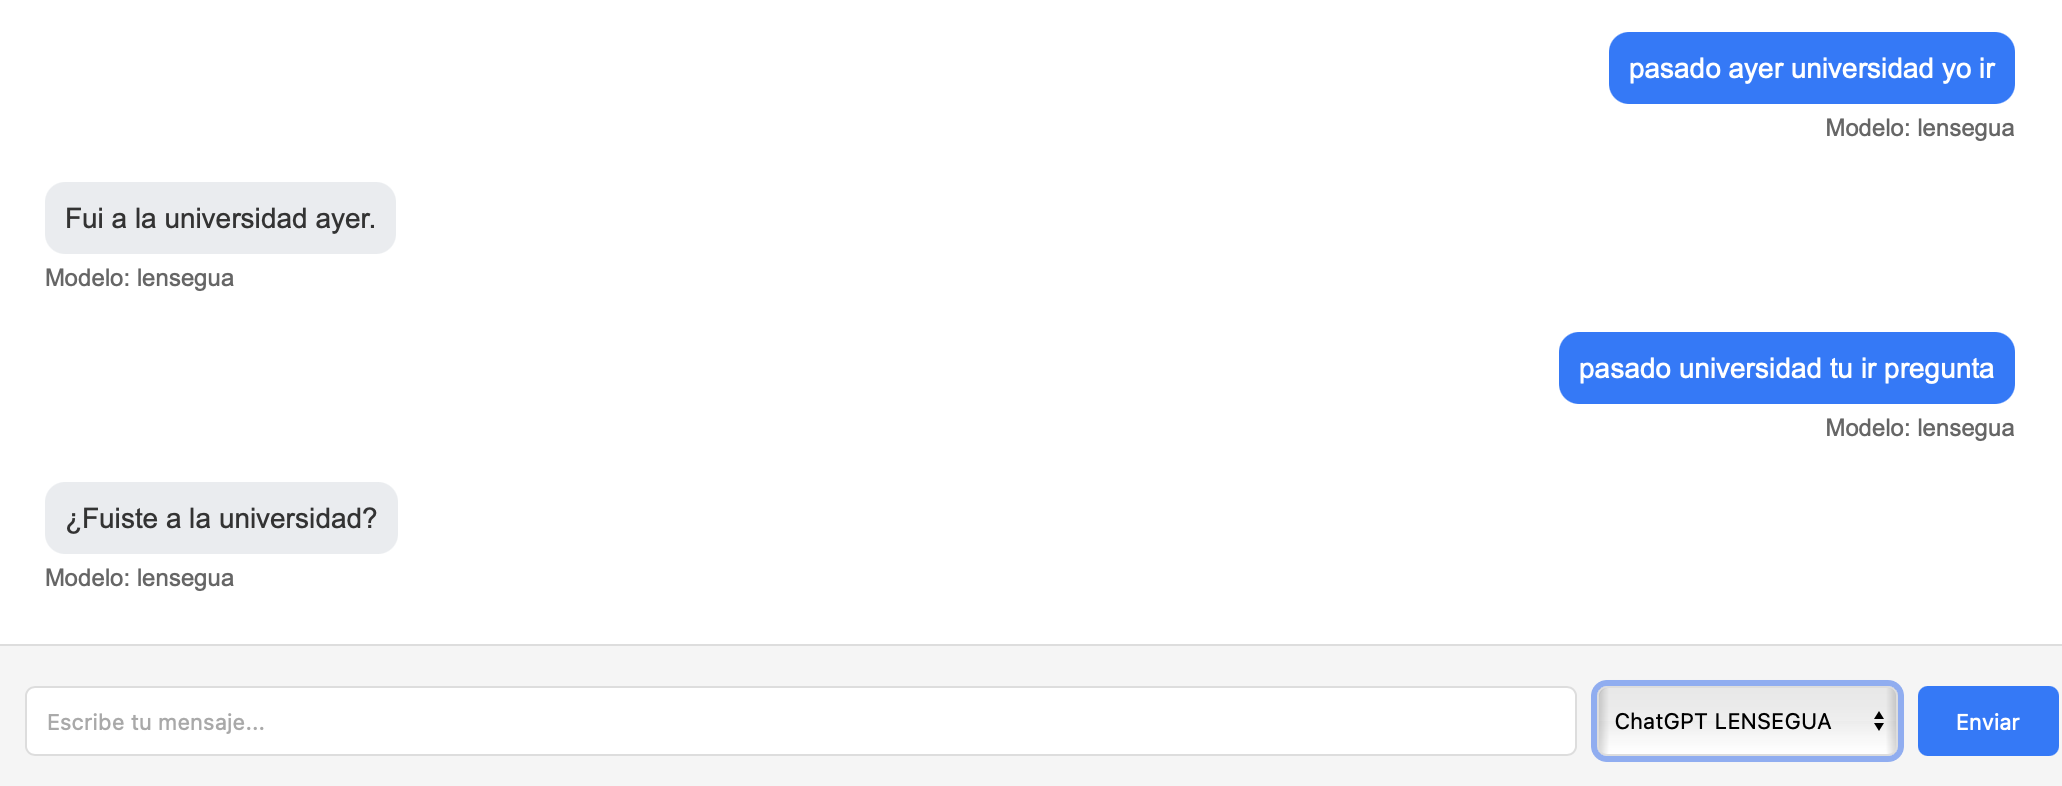
\includegraphics[width=1\linewidth]{figuras/lensegua-web.png}
\caption{Aplicación web desarrollada para facilitar interacción con modelo \textit{fine-tuneado}.}
\label{fig:web}
\end{figure}


Para complementar la evaluación, se llevó a cabo una encuesta en Google Forms, que fue respondida no solo por los participantes de la reunión en En-Señas, sino también por otras personas sordas, intérpretes, estudiantes y usuarios familiarizados con LENSEGUA. En esta encuesta, un total de 19 personas evaluaron las interpretaciones generadas por ambos modelos en una escala del 1 al 5, donde 1 correspondía a menor coherencia y 5 a mayor coherencia o claridad. Cabe resaltar que dichas interpretaciones se generaron utilizando la quinta versión del \textit{prompt} desarrollado.

En este contexto, la Tabla \ref{tab:R1} presenta un ejemplo comparativo de las interpretaciones de la frase “ayer cine tu ir pregunta”. El modelo original generó la interpretación “Ayer fuiste al cine, ¿verdad?”, y obtuvo una puntuación promedio de 3.4. En cambio, el modelo \textit{fine-tuneado} interpretó la frase como “¿Fuiste al cine ayer?”, alcanzando una puntuación de 4.8. Los 19 participantes estuvieron de acuerdo en que la interpretación del modelo \textit{fine-tuneado} fue más precisa y adecuada.

\vspace{0.5cm}
\begin{table}[H]
\centering
    \begin{tabular}{|l|p{7cm}|c|}
        \hline
        \multicolumn{3}{|l|}{\textbf{Frase en LENSEGUA:} ayer cine tu ir pregunta} \\ \hline \hline
        \textbf{Modelo} & \textbf{Interpretación} & \textbf{Puntuación Promedio} \\ \hline
        GPT-3.5-Turbo & Ayer fuiste al cine, ¿verdad? & 3.4 \\ \hline
        \textit{Fine-Tuneado} & ¿Fuiste al cine ayer? & 4.8 \\ \hline
    \end{tabular}
    \caption{Puntuación promedio otorgada por usuarios finales a las interpretaciones generadas por el modelo GPT-3.5-Turbo estándar y su versión \textit{fine-tuneada} para la frase “ayer cine tu ir pregunta”.}
    \label{tab:R1}
\end{table}

En la Tabla \ref{tab:R2} se analiza la frase “pasado yo medicina comprar para mamá”. El modelo original generó la interpretación “En el pasado compré medicina para mi mamá”, obteniendo una puntuación promedio de 3.8. Por su parte, el modelo \textit{fine-tuneado} simplificó la interpretación a “Compré medicina para mi mamá”, logrando una puntuación de 4.9. Si bien ambas interpretaciones son correctas, todos los participantes coincidieron en que la del modelo \textit{fine-tuneado} fue más apropiada. Esto probablemente debido a que el modelo original añadió información -“en el pasado”- que suele omitirse.

\vspace{0.5cm}
\begin{table}[H]
\centering
    \begin{tabular}{|l|p{7cm}|c|}
        \hline
        \multicolumn{3}{|l|}{\textbf{Frase en LENSEGUA:} pasado yo medicina comprar para mamá} \\ \hline \hline
        \textbf{Modelo} & \textbf{Interpretación} & \textbf{Puntuación Promedio} \\ \hline
        GPT-3.5-Turbo & En el pasado compré medicina para mi mamá. & 3.8 \\ \hline
        \textit{Fine-Tuneado} & Compré medicina para mi mamá. & 4.9 \\ \hline
    \end{tabular}
    \caption{Puntuación promedio otorgada por usuarios finales a las interpretaciones generadas por el modelo GPT-3.5-Turbo estándar y su versión \textit{fine-tuneada} para la frase “pasado yo medicina comprar para mamá”.}
    \label{tab:R2}
\end{table}

La Tabla \ref{tab:R3} presenta los resultados para la frase “ayer abuelo llamar tu pregunta”. El modelo original generó “Ayer tu abuelo te llamó para preguntarte algo”, y obtuvo una puntuación de 1.8. En contraste, el modelo \textit{fine-tuneado} generó la frase “¿Ayer te llamó tu abuelo?”, obteniendo 4.9 puntos. Los participantes seleccionaron esta última interpretación como la más clara y correcta, posiblemente ya que capturaba de manera más fiel la idea que se buscaba transmitir.

\vspace{0.5cm}
\begin{table}[H]
\centering
    \begin{tabular}{|l|p{7cm}|c|}
        \hline
        \multicolumn{3}{|l|}{\textbf{Frase en LENSEGUA:} ayer abuelo llamar tu pregunta} \\ \hline \hline
        \textbf{Modelo} & \textbf{Interpretación} & \textbf{Puntuación Promedio} \\ \hline
        GPT-3.5-Turbo & Ayer tu abuelo te llamó para preguntarte algo. & 1.8 \\ \hline
        \textit{Fine-Tuneado} & ¿Ayer te llamó tu abuelo? & 4.9 \\ \hline
    \end{tabular}
    \caption{Puntuación promedio otorgada por usuarios finales a las interpretaciones generadas por el modelo GPT-3.5-Turbo estándar y su versión \textit{fine-tuneada} para la frase “ayer abuelo llamar tu pregunta”.}
    \label{tab:R3}
\end{table}

En la Tabla \ref{tab:R4} se muestra la evaluación de la frase “antes tienda tu amiga ver pregunta”. El modelo original generó “Tu amiga vio la tienda y te preguntó algo”, y obtuvo una puntuación de 1.4. El modelo \textit{fine-tuneado} produjo “¿Viste a tu amiga en la tienda?”, alcanzando 4.1 puntos. Nuevamente, todos los participantes coincidieron en que la interpretación generada por el modelo adaptado era la más clara y coherente.

\vspace{0.5cm}
\begin{table}[H]
\centering
    \begin{tabular}{|l|p{7cm}|c|}
        \hline
        \multicolumn{3}{|l|}{\textbf{Frase en LENSEGUA:} antes tienda tu amiga ver pregunta} \\ \hline \hline
        \textbf{Modelo} & \textbf{Interpretación} & \textbf{Puntuación Promedio} \\ \hline
        GPT-3.5-Turbo & Tu amiga vio la tienda y te preguntó algo. & 1.4 \\ \hline
        \textit{Fine-Tuneado} & ¿Viste a tu amiga en la tienda? & 4.1 \\ \hline
    \end{tabular}
    \caption{Puntuación promedio otorgada por usuarios finales a las interpretaciones generadas por el modelo GPT-3.5-Turbo estándar y su versión \textit{fine-tuneada} para la frase “antes tienda tu amiga ver pregunta”.}
    \label{tab:R4}
\end{table}

Finalmente, en la Tabla \ref{tab:R5} se analiza la frase “tu opinión cuál pregunta”. El modelo original la interpretó como “Tu opinión sobre cuál es la pregunta”, obteniendo 1.4 puntos. Por otro lado, el modelo \textit{fine-tuneado} generó “¿Cuál es tu opinión?”, logrando la máxima puntuación de 5.0 puntos. Todos los participantes estuvieron de acuerdo en que esta última interpretación fue la más adecuada.

\vspace{0.5cm}
\begin{table}[H]
\centering
    \begin{tabular}{|l|p{7cm}|c|}
        \hline
        \multicolumn{3}{|l|}{\textbf{Frase en LENSEGUA:} tu opinión cuál pregunta} \\ \hline \hline
        \textbf{Modelo} & \textbf{Interpretación} & \textbf{Puntuación Promedio} \\ \hline
        GPT-3.5-Turbo & Tu opinión sobre cuál es la pregunta. & 1.4 \\ \hline
        \textit{Fine-Tuneado} & ¿Cuál es tu opinión? & 5.0 \\ \hline
    \end{tabular}
    \caption{Puntuación promedio otorgada por usuarios finales a las interpretaciones generadas por el modelo GPT-3.5-Turbo estándar y su versión \textit{fine-tuneada} para la frase “tu opinión cuál pregunta”.}
    \label{tab:R5}
\end{table}

En la última fase de la encuesta, se solicitó a los participantes evaluar cinco interpretaciones de una misma frase. Cada una de las interpretaciones fue generada utilizando un \textit{prompt} distinto, en conjunto con el modelo \textit{fine-tuneado}. El objetivo fue identificar cuál de los cinco \textit{prompts} producía la interpretación más adecuada y coherente según personas conocedoras de la gramática de LENSEGUA. 

Como se puede observar en la Tabla \ref{tab:R6}, las primeras tres interpretaciones obtuvieron calificaciones promedio bajas (1.4, 1.1 y 1.4, respectivamente), ya que no lograron transmitir correctamente la idea original y contenían errores. En lugar de indicar que se esperaba que no hubiera tráfico, estas interpretaciones mencionaron lo opuesto, lo que distorsionó el mensaje. Por otro lado, la cuarta y quinta versión generaron interpretaciones mucho más adecuadas y claras, logrando transmitir el mensaje de manera efectiva. Es importante mencionar que estas últimas dos interpretaciones eran muy similares; sin embargo, debido a ligeras variaciones en la redacción, los usuarios indicaron que la interpretación generada por el quinto \textit{prompt} fue superior, obteniendo una puntuación promedio de 5.0.

Finalmente, de los 19 participantes, 18 eligieron la interpretación generada con el quinto \textit{prompt} como su favorita, mientras que solo uno optó por la interpretación generada con el  cuarto \textit{prompt}. Este resultado no solo sugiere que el quinto \textit{prompt} fue el más efectivo, sino que también coincide con las puntuaciones de distancia de Levenshtein promedio mencionadas anteriormente. 

\vspace{0.5cm}
\begin{table}[H]
\centering
    \begin{tabular}{|l|p{8cm}|c|}
        \hline
        \multicolumn{3}{|l|}{\textbf{Frase en LENSEGUA:} hospital yo necesitar ir ahora ojalá mucho carro no porque emergencia} \\ \hline \hline
        \textbf{\textit{Prompt}} & \textbf{Interpretación} & \textbf{Puntuación Promedio} \\ \hline
        Versión 1 & Necesito ir al hospital ahora espero que haya muchos carros porque es una emergencia. & 1.4 \\ \hline
        Versión 2 & Necesito ir al hospital ahora espero que haya muchos carros disponibles no tengo carro porque es una emergencia. & 1.1 \\ \hline
        Versión 3 & Necesito ir al hospital ahora porque es una emergencia y ojalá haya mucho carro. & 1.4 \\ \hline
        Versión 4 & Necesito ir al hospital ahora espero que no haya mucho tráfico porque es una emergencia. & 4.6 \\ \hline
        Versión 5 & Necesito ir al hospital ahora mismo. Espero que no haya mucho tráfico porque es una emergencia. & 5.0 \\ \hline

    \end{tabular}
    \caption{Puntuación promedio otorgada por usuarios finales a las interpretaciones generadas por el modelo GPT-3.5-Turbo \textit{fine-tuneado}, utilizando diferentes \textit{prompts}, para la frase “hospital yo necesitar ir ahora ojalá mucho carro no porque emergencia”.}
    \label{tab:R6}
\end{table}














% Modulo de LLaMA
\section{Procesamiento de lenguaje natural (LLaMA)} 

\subsection{Fine-tuning (versión 1)}

Para encontrar la configuración óptima del modelo LLaMA en la tarea de interpretación de LENSEGUA, se realizaron varios experimentos preliminares utilizando una porción del \textit{dataset}. Estos experimentos se centraron en identificar las configuraciones que generaban el mejor modelo en términos de pérdida de validación y de la métrica BLEU promedio.

En el primer experimento, se entrenó un modelo sin ajustes específicos para verificar su funcionamiento básico. Como se observa en la Figura \ref{fig:LLAMAm1}, existía una tendencia al sobreentrenamiento, resultando en un valor BLEU promedio de 0.125, lo cual indicaba interpretaciones deficientes.

\vspace{0.5cm}
\begin{figure}[H]
\centering
	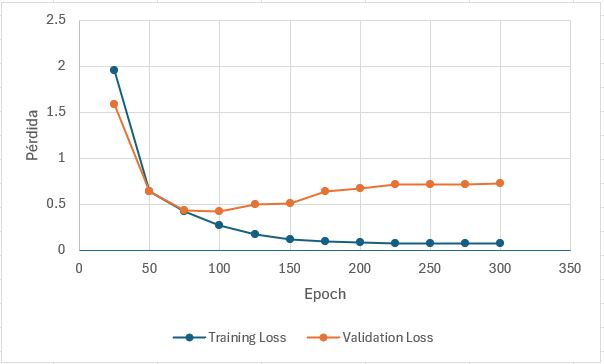
\includegraphics[height=5.5 cm]{figuras/Resultado1.JPG}
    \caption{Evolución de la pérdida durante el \textit{fine-tuning} del modelo LLaMA preliminar.}
    \label{fig:LLAMAm1}
\end{figure}


Para abordar este problema, se implementó la técnica de \textit{early stopping} en el segundo experimento, reduciendo los \textit{batches} de entrenamiento de 300 a 100. La Figura \ref{fig:LLAMAm2} muestra la evolución de la pérdida durante este experimento, evidenciando una mejora significativa en la generalización del modelo. Se alcanzó un valor BLEU promedio de 0.212, lo cual refleja una mejora en la calidad de las predicciones generadas por el modelo. 

\vspace{0.5cm}
\begin{figure}[H]
\centering
	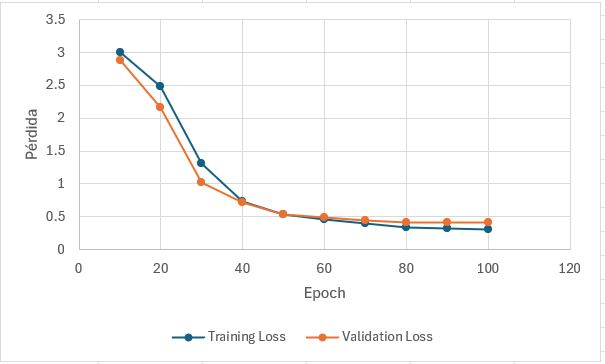
\includegraphics[height=5.5 cm]{figuras/Resultado2.JPG}
    \caption{Evolución de la pérdida durante el \textit{fine-tuning} del modelo LLaMA con \textit{early stopping}.}
    \label{fig:LLAMAm2}
\end{figure}

Es importante mencionar que en todas las pruebas se utilizó LoRA. Sin embargo, durante el tercer experimento, se implementó una configuración estándar de LoRA, ajustando los parámetros de rango y alpha a valores de 8 y 16, respectivamente, siguiendo las recomendaciones de un estudio de traducción bilingüe \cite{weller2022pretrained}. La Figura \ref{fig:LLAMAm3} muestra cómo esta configuración, junto con el \textit{early stopping}, resultó en una mejora en la pérdida del modelo. Este ajuste contribuyó a obtener un valor BLEU promedio de 0.239, representando un avance significativo respecto a los experimentos anteriores.

\vspace{0.5cm}
\begin{figure}[H]
\centering
	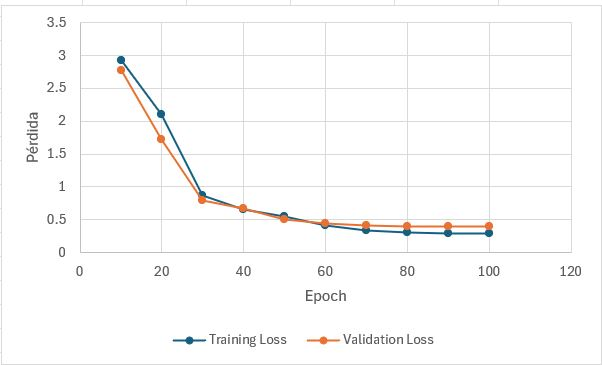
\includegraphics[height=5.5 cm]{figuras/Resultado3.JPG}
    \caption{Evolución de la pérdida durante el \textit{fine-tuning} del modelo LLaMA con \textit{early stopping} y estándar LoRA.}
    \label{fig:LLAMAm3}
\end{figure}

Finalmente, en el cuarto experimento, se tomó la decisión de reducir la flexibilidad del modelo al pasar a un enfoque más estricto de \textit{fine-tuning} supervisado. Es decir, se forzó al modelo a entrenar completamente bajo supervisión, eliminando la capacidad de decidir si entrenar de forma supervisada o no. A pesar de este cambio, se mantuvo el estándar de LoRA y se continuó utilizando la técnica de \textit{early stopping}. Este ajuste alcanzó un valor BLEU promedio de 0.263, estableciendo el mejor rendimiento observado hasta el momento.

\vspace{0.5cm}
\begin{figure}[H]
\centering
	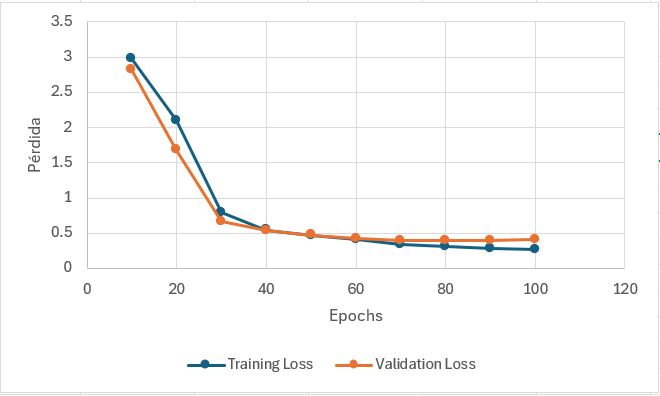
\includegraphics[height=5.5 cm]{figuras/Resultado4.JPG}
    \caption{Evolución de la pérdida durante el \textit{fine-tuning} del modelo LLaMA con \textit{early stopping}, estándar LoRA y \textit{fine-tuning} supervisado.}
    \label{fig:LLAMAm4}
\end{figure}


La Tabla \ref{tab:BLEUmodelos} resume los resultados de estos experimentos preliminares, mostrando la progresión en el rendimiento del modelo con cada modificación implementada. Basándose en estos resultados, se seleccionó la configuración del cuarto experimento para realizar un entrenamiento final utilizando el conjunto completo de datos. Este entrenamiento permitió aumentar el valor BLEU promedio a 0.2894, lo cual confirma que la combinación de \textit{early stopping}, estándar LoRA y un enfoque de \textit{fine-tuning} supervisado estricto era la más adecuada para esta tarea.

\vspace{0.5cm}
\begin{table}[H]
    \centering
    \begin{tabular}{|l|c|}
        \hline
        \textbf{Modelo} & \textbf{BLEU promedio} \\
        \hline
        Modelo predeterminado & 0.125 \\
        \hline
        Modelo con \textit{early stopping} & 0.212\\
        \hline
        Modelo con \textit{early stopping} y estándar LoRA & 0.239\\
        \hline
        Modelo con \textit{early stopping}, estándar LoRA y \textit{fine-tuning} supervisado & 0.263 \\
        \hline
    \end{tabular}
    \caption{Valores promedio de BLEU en experimentos preliminares.}
    \label{tab:BLEUmodelos}
\end{table}

Para evaluar el rendimiento específico del modelo, se analizaron tres oraciones de prueba, cuyos resultados se presentan en la Tabla \ref{tab:oracionesBLEU}. Los valores BLEU variaron significativamente entre 1.0, 0.0 y 0.5, proporcionando información valiosa sobre la capacidad del modelo para manejar diferentes tipos de oraciones.

\vspace{0.5cm}
\begin{table}[H]
    \centering
    \begin{tabular}{|l|l|c|}
        \hline
        \textbf{Interpretación Esperada} & \textbf{Interpretación Real} & \textbf{BLEU} \\
        \hline
        ¿Como esta el día hoy? & ¿Como esta el día hoy? & 1.0 \\
        \hline
        Miguel gana la carrera. & Miguel gano la carrera. & 0.0\\
        \hline
        Pon la flor azul sobre la mesa. & Pon la flor azul en la mesa & 0.5 \\
        \hline
    \end{tabular}
    \caption{Valores BLEU de interpretaciones generadas por el modelo LLaMA con \textit{early stopping}, estándar LoRA y \textit{fine-tuning} supervisado.}
    \label{tab:oracionesBLEU}
\end{table}


Tras completar el proceso de \textit{fine-tuning} final, se aplicó la técnica de \textit{Local Interpretable Model-agnostic Explanations} (LIME) para evaluar el impacto de este proceso en las interpretaciones generadas por el modelo. Esta técnica permitió identificar las palabras clave que ejercían mayor influencia en las interpretaciones generadas para frases específicas, proporcionando una visión más clara y detallada sobre cómo el modelo procesa y utiliza la información para generar sus predicciones. Para este análisis, se seleccionaron tres frases representativas, lo que permitió explorar diferentes escenarios lingüísticos y evaluar el desempeño del modelo en contextos variados.

Dado que se empleó la librería de transformadores para este análisis, fue necesario trabajar con valores de logits y atenciones del transformador. Estos valores, aunque pequeños en magnitud, representan la importancia relativa de cada palabra en la interpretación final. Los logits y las atenciones reflejan la medida en que el modelo se enfoca en ciertos términos y su relevancia en la interpretación.

En la Figura \ref{fig:LIME1-LLAMA1}, el análisis LIME para la frase “como clima hoy” muestra el impacto de las palabras y cómo estas influyen en la interpretación final generada por el modelo. Todos los valores son positivos, lo que indica que las palabras fueron entendidas y contribuyeron significativamente a la construcción de la interpretación, permitiendo resultados más precisos.

En esta figura, se observa que la palabra “como” obtuvo un el mayor impacto, posiblemente debido a que el modelo reconoció que esta palabra representaba una pregunta. La referencia temporal con “hoy” y el término “clima” complementaron la construcción de la interpretación. En la Tabla \ref{tab:LIME1-LLAMA1} se presentan los resultados numéricos del análisis LIME.


\begin{figure}[H]
\centering
    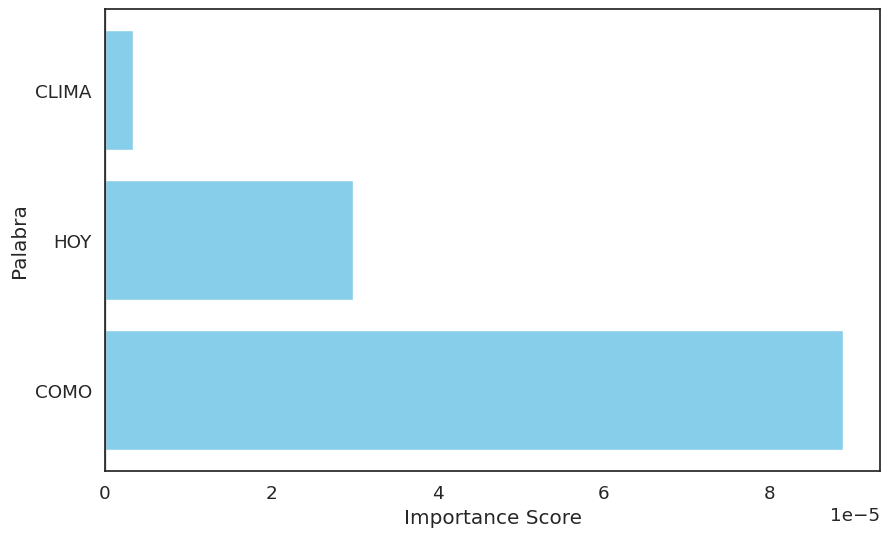
\includegraphics[width=0.7\textwidth]{figuras/Oracion1.png}
    \caption{Resultados de LIME para la interpretación generada por el modelo LLaMA \textit{fine-tuneado} (versión 1) para la frase “como clima hoy”.}
    \label{fig:LIME1-LLAMA1}
\end{figure}


\vspace{0.5cm}
\begin{table}[H]
\centering
    \begin{tabular}{|l|c|c|}
        \hline
        \multicolumn{2}{|l|}{\textbf{Frase en LENSEGUA:} como clima hoy} \\ \hline
        \multicolumn{2}{|l|}{\textbf{Interpretación teórica:} ¿Cómo está el clima hoy?} \\ \hline \hline
        
        \textbf{Palabra} & \multicolumn{1}{c|}{\textbf{Valores de Influencia (LIME)}} \\ 
        \cline{3-0} & \textbf{Modelo \textit{fine-tuneado}} \\
         
        \hline
        COMO  & 9.246e-05  \\ \hline
        HOY & 3.395e-06 \\ \hline
        CLIMA & 7.904e-07 \\ \hline
        
    \end{tabular}
\caption{Contribución de cada palabra según los Valores de Influencia (LIME) en las interpretaciones generadas por el modelo LLaMA \textit{fine-tuneado} (versión 1) para la frase “como clima hoy”.}
\label{tab:LIME1-LLAMA1}
\end{table}


En la Figura \ref{fig:LIME1-LLAMA2}, se analiza la frase “ayer viernes limpiar casa todo día”. Similarmente a la Figura anterior, todas las palabras tienen valores positivos, destacando términos como “día”, “todo” y “ayer” por su mayor relevancia. En este caso, las referencias temporales fueron mejor interpretadas, mientras que la acción “limpiar” presentó un menor valor de importancia.

\begin{figure}[H]
\centering
    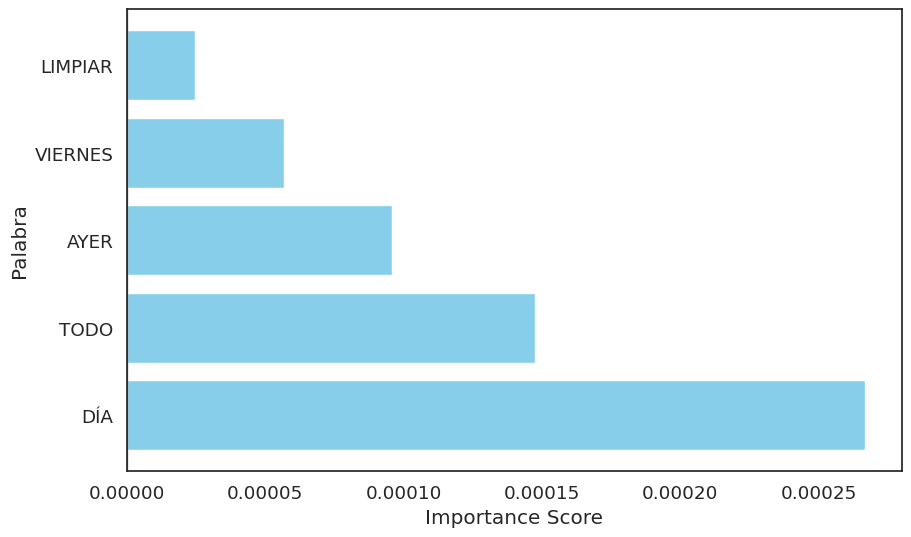
\includegraphics[width=0.7\textwidth]{figuras/Oracion2.png}
    \caption{Resultados de LIME para la interpretación generada por el modelo LLaMA \textit{fine-tuneado} (versión 1) para la frase “ayer viernes limpiar casa todo día”.}
    \label{fig:LIME1-LLAMA2}
\end{figure}


\vspace{0.5cm}
\begin{table}[H]
\centering
    \begin{tabular}{|l|c|c|}
        \hline
        \multicolumn{2}{|l|}{\textbf{Frase en LENSEGUA:} ayer viernes limpiar casa todo día} \\ \hline
        \multicolumn{2}{|l|}{\textbf{Interpretación teórica:} Ayer viernes limpié la casa todo el día.} \\ \hline \hline
        
        \textbf{Palabra} & \multicolumn{1}{c|}{\textbf{Valores de Influencia (LIME)}} \\ 
        \cline{3-0} & \textbf{Modelo \textit{fine-tuneado}} \\
         
        \hline
        DÍA & 2.666e-4  \\ 
        \hline
        TODO & 1.475e-4 \\
        \hline
        AYER & 9.583e-05 \\
        \hline
        VIERNES & 5.679e-05\\
        \hline 
        LIMPIAR & 2.4804e-05\\
        \hline
        
    \end{tabular}
\caption{Contribución de cada palabra según los Valores de Influencia (LIME) en las interpretaciones generadas por el modelo LLaMA \textit{fine-tuneado} (versión 1) para la frase “ayer viernes limpiar casa todo día”.}
\label{tab:LIME1-LLAMA2}
\end{table}


Finalmente, en la Figura \ref{fig:LIME1-LLAMA3}, se analiza la frase “mar gustar él mar gustar ella no”. Este caso incluye una oración más larga y contiene una palabra repetida. El análisis muestra que la palabra repetida tiene menor importancia, mientras que el término “no” es crucial para establecer la distinción entre las dos entidades mencionadas. Sin embargo, se evidencia cierta confusión por parte del modelo con la palabra “ella”, que representa una entidad diferente.



\begin{figure}[H]
\centering
    \includegraphics[width=0.7\textwidth]{figuras/Oracion3.png}
    \caption{Resultados de LIME para la interpretación generada por el modelo LLaMA \textit{fine-tuneado} (versión 1) para la frase “mar gusta él mar gustar ella no”.}
    \label{fig:LIME1-LLAMA3}
\end{figure}


\vspace{0.5cm}
\begin{table}[H]
\centering
    \begin{tabular}{|l|c|c|}
        \hline
        \multicolumn{2}{|l|}{\textbf{Frase en LENSEGUA:} mar gusta él mar gustar ella no} \\ \hline
        \multicolumn{2}{|l|}{\textbf{Interpretación teórica:} A él le gusta el mar, pero a ella no.} \\ \hline \hline
        
        \textbf{Palabra} & \multicolumn{1}{c|}{\textbf{Valores de Influencia (LIME)}} \\ 
        \cline{3-0} & \textbf{Modelo \textit{fine-tuneado}} \\
         
        \hline
        NO  & 2.393e-05  \\ \hline
        ELLA & -1.329e-05 \\
        \hline
        GUSTAR & 1.181e-06 \\
        \hline
        ÉL & 8.746e-07\\
        \hline 
        MAR & 4.894e-08\\
        \hline
        
    \end{tabular}
\caption{Contribución de cada palabra según los Valores de Influencia (LIME) en las interpretaciones generadas por el modelo LLaMA \textit{fine-tuneado} (versión 1) para la frase “mar gusta él mar gustar ella no”.}
\label{tab:LIME1-LLAMA3}
\end{table}





\subsection{Retroalimentación de la comunidad sorda}

Al finalizar el entrenamiento, los resultados finales del \textit{fine-tuning} se presentaron a una experta en LENSEGUA, quien evaluó las interpretaciones generadas por el modelo. Durante esta entrevista se analizaron diversas traducciones, destacando aspectos positivos y áreas de mejora. La Tabla \ref{tab:LAMMA-Entr} resume los comentarios proporcionados.

\vspace{0.5cm}
\begin{table}[H]
\centering
    \begin{tabular}{|p{4cm}|p{4cm}|p{4cm}|}
        \hline
        \textbf{Interpretación teórica} & \textbf{Interpretación real} & \textbf{Comentario} \\
        \hline
        ¿Ustedes comen pastel? & Ustedes comieron pastel & La oración en sí esta bien. Sin embargo, esta en forma de interrogación, lo que no es según los signos específicas. Se necesita especificar con signos de puntuación.\\
        \hline
        El eligió entre dos casas. & El elige entre dos casas. &  Buy buena traducción. Se guarda la presencia de la información. Lo que sí, es que esta en pasado la oración tradución. En las frases, no hay ninga referencia de la acción esta en pasado o presente.\\
        \hline
        A Juan no le gusta leer. & A Juan no le gusta leer. & Una traducción bastante perfecta. Guarda la información y tiene sentido con respecto a las señas utilizadas.\\
        \hline
        Pon la flor azul sobre la mesa. & Pon la flor azul en la mesa. & La traducción esta muy buena y es de alta cálidad. Lo que hay que tener en mente es que en LENSEGUA, no existén los arítculos o prepocisiones, estos hay que inferirlos basados en las señas, y estas cambian basado en la interpretación de la persona. \\  
        \hline
        SACAGRAPAS & Sacagawea & Esta traducción esta basante mal. Se tiene la idea, pero las letras no coinciden con lo que se quiere decir exactamente. \\  
                \hline
        La pizza de queso es mi favorita. & Pizzo es mi queso favorite & Hay una idea general de lo que se quiera hablar, que es el queso favorito. Sin embargo, esta a media la oración, y a pesar que la esencia básica esta ahí, no es acceptable de la misma manera y hay que mejorar en la base de datos para poder mejorar el resultado final. \\  
        \hline
    \end{tabular}
    \caption{Comentarios otorgados por un intérprete de LENSEGUA ante interpretaciones generadas por el modelo LLaMA \textit{fine-tuneado} (versión 1) para diversas frases.}
\label{tab:LAMMA-Entr}
\end{table}
\vspace{0.5cm}

Uno de los puntos clave mencionados fue la dificultad del modelo para diferenciar entre preguntas y declaraciones. Por ejemplo, en la oración “¿Ustedes comen pastel?”, la interpretación generada fue “Ustedes comieron pastel”, lo cual no respeta el formato interrogativo. La experta recomendó incorporar marcadores específicos en el conjunto de datos para que el modelo pueda identificar adecuadamente el tipo de enunciado, evitando así confusiones. 

Otro aspecto señalado fue la inconsistencia en los tiempos verbales. En la frase “Él eligió entre dos casas”, la traducción generada estuvo en presente, “Él elige entre dos casas”, en lugar de pasado. Esto refleja la necesidad de enriquecer el conjunto de datos con información que especifique el tiempo verbal, lo que permitiría obtener interpretaciones más precisas y acordes al contexto original. 

Asimismo, se identificaron errores en algunas traducciones, como el caso de “SACAGRAPAS”, donde la interpretación fue “Sacagawea”, lo que muestra una falta de coincidencia entre las letras esperadas y las generadas. La experta destacó la importancia de mejorar la calidad y diversidad del conjunto de datos para abordar estos problemas y reducir la incidencia de errores. A pesar de estas limitaciones, ella reconoció que la mayoría de las interpretaciones eran comprensibles y lograban transmitir el significado general esperado. En palabras de la experta: “ambas dicen lo mismo, solo que de maneras diferentes”. Esto refleja que, aunque las traducciones podían diferir en estructura o formato, conservaban la esencia básica de LENSEGUA.

Finalmente, la experta otorgó una calificación de 9 sobre 10 a las traducciones generadas por el modelo, considerando que el contenido reflejaba de manera adecuada el contexto de la lengua de señas. Este puntaje positivo resalta la calidad general de las interpretaciones y su coherencia con las señas utilizadas, aunque subraya la importancia de seguir mejorando aspectos como la diferenciación de enunciados, la consistencia en tiempos verbales y la precisión en palabras específicas.


\subsection{Fine-tuning (versión 2)}

Los resultados del modelo LLaMA \textit{fine-tuneado} (versión 1) mostraron un desempeño aceptable; sin embargo, con base en las métricas y comentarios obtenidos en la entrevista con la experta en LENSEGUA, se identificó la oportunidad de mejorar las métricas mediante un proceso de \textit{fine-tuning} más exhaustivo. Manteniendo la misma configuración óptima previamente identificada, se llevó a cabo una nueva tarea de \textit{fine-tuning} utilizando un conjunto de datos específicamente desarrollado para el modelo GPT-3.5-Turbo. Este conjunto de datos constaba de 4,192 entradas para entrenamiento y 200 entradas de validación.

A partir de este proceso, se observó una mejora sustancial en la métrica BLEU promedio del modelo, que pasó de 0.2894, obtenida con el conjunto de datos anterior, a 0.632 con el nuevo conjunto de datos. Esta mejora sustancial indica que el modelo es capaz de generar interpretaciones más cercanas a las referencias teóricas establecidas. 

Dado que los modelos LLaMA (versión 2) y GPT-3.5-Turbo fueron entrenados con el mismo conjunto de datos, se decidió comparar su rendimiento utilizando la distancia de Levenshtein y el largo promedio de las interpretaciones. Como se observa en la Tabla \ref{tab:LEVENSHTEIN-COMP}, LLaMA generó interpretaciones con un promedio de 28.65 palabras y una distancia de Levenshtein de 6.185. Por otro lado, GPT-3.5-Turbo produjo interpretaciones más cercanas a las teóricas, con un promedio de 26.635 palabras y una distancia promedio menor de 3.375.

\vspace{0.5cm}
\begin{table}[H]
\centering
    \begin{tabular}{|l|c|c|c|}
        \hline
        \textbf{Modelo} & \textbf{Largo promedio} & \textbf{Distancia de} & \textbf{Porcentaje de} \\ 
        & \textbf{de interpretaciones} & \textbf{Levenshtein promedio} & \textbf{Diferencia} \\ \hline

        LLaMa 3.0 (versión 2) & 28.65 & 6.185 & 15.27\%\\
        \hline
        GPT-3.5-Turbo & 26.635 & 3.375 & 11.98\%\\
        \hline
        
    \end{tabular}
    \caption{Distancias de Levenshtein promedio calculadas a partir de las interpretaciones generadas por el modelo GPT-3.5-Turbo \textit{fine-tuneado} y el modelo LLaMA \textit{fine-tuneado} (versión 2)}
    \label{tab:LEVENSHTEIN-COMP}
\end{table}

Para profundizar en el análisis del comportamiento del modelo, se aplicó la técnica LIME al modelo LLaMA (versión 2), cuyos resultados se visualizan en las Figuras \ref{fig:LIME2-F1}, \ref{fig:LIME2-F2} y \ref{fig:LIME2-F3}. Además, se realizó una comparación con los valores de influencia LIME obtenidos con el modelo GPT-3.5-Turbo, presentados en las Tablas \ref{tab:LIME2-1}, \ref{tab:LIME2-2} y \ref{tab:LIME2-3}. Esta comparación permitió entender cómo cada modelo asignaba diferentes niveles de relevancia a las palabras durante el proceso de interpretación.

En el análisis de la frase “ojalá hoy carro mucho no”, como se muestra en la Figura \ref{fig:LIME2-F1}, el modelo LLaMA identificó “ojalá” como la palabra más influyente con un valor de 0.12, seguida por “hoy” con 0.05. La Tabla \ref{tab:LIME2-1} revela que GPT-3.5-Turbo asignó la mayor relevancia a “hoy” con 0.34, seguido por “ojalá” con 0.19 y “carro” con 0.13, mostrando una distribución diferente de la importancia entre los elementos temporales y contextuales de la frase.

\begin{figure}[H]
\centering
    \includegraphics[width=0.7\textwidth]{figuras/Oracion1.JPG}
    \caption{Resultados de LIME para la interpretación generada por el modelo LLaMA \textit{fine-tuneado} (versión 2) para la frase “ojalá hoy carro mucho no”.}
    \label{fig:LIME2-F1}
\end{figure}

\vspace{0.5cm}
\begin{table}[H]
\centering
    \begin{tabular}{|l|c|c|}
        \hline
        \multicolumn{3}{|l|}{\textbf{Frase en LENSEGUA:} ojalá hoy carro mucho no} \\ \hline
        \multicolumn{3}{|l|}{\textbf{Interpretación teórica:} Espero que no haya tráfico hoy.} \\ \hline \hline
        
        \textbf{Palabra} & \multicolumn{2}{c|}{\textbf{Valores de Influencia (LIME)}} \\ 
        \cline{2-3}
        & \textbf{LLaMA \textit{fine-tuneado} (versión 2)} & \textbf{GPT-3.5-Turbo \textit{fine-tuneado}} \\
         
        \hline
        ojalá & 0.12 & 0.19 \\
        \hline
        hoy & 0.05 & 0.34 \\
        \hline
        carro & 0.03  & 0.13 \\
        \hline
        mucho & 0.02  & 0.09 \\
        \hline
        no & 0.01  & 0.02 \\
        \hline
        
    \end{tabular}
\caption{Contribución de cada palabra según los Valores de Influencia (LIME) en las interpretaciones generadas por el modelo LLaMA \textit{fine-tuneado} (versión 2) y el modelo GPT-3.5-Turbo \textit{fine-tuneado} para la frase “ojalá hoy carro mucho no”.}
\label{tab:LIME2-1}
\end{table}

Para la segunda frase analizada, “antes tu policía llamar pregunta”, se observa una distribución uniforme de la influencia entre todas las palabras, con valores entre 0.00 y 0.02. Al examinar la Tabla \ref{tab:LIME2-2}, se evidencia que GPT-3.5-Turbo asignó valores de influencia significativamente más altos a palabras específicas: “policía” con 0.43 y “llamar” con 0.20, mientras que las demás palabras mantuvieron valores por debajo de 0.10. Esto último sugiere que el modelo GPT-3.5-Turbo tiene una mejor comprensión de los elementos clave en la frase.

\begin{figure}[H]
\centering
    \includegraphics[width=0.7\textwidth]{figuras/Oracion2.JPG}
    \caption{Resultados de LIME para la interpretación generada por el modelo LLaMA \textit{fine-tuneado} (versión 2) para la frase “antes tu policía llamar pregunta”.}
    \label{fig:LIME2-F2}
\end{figure}

\vspace{0.5cm}
\begin{table}[H]
\centering
    \begin{tabular}{|l|c|c|}
        \hline
        \multicolumn{3}{|l|}{\textbf{Frase en LENSEGUA:} antes tu policía llamar pregunta} \\ \hline
        \multicolumn{3}{|l|}{\textbf{Interpretación teórica:} ¿Llamaste a la policía?} \\ \hline \hline
        
        \textbf{Palabra} & \multicolumn{2}{c|}{\textbf{Valores de Influencia (LIME)}} \\ 
        \cline{2-3}
        & \textbf{LLaMA \textit{fine-tuneado} (versión 2)} & \textbf{GPT-3.5-Turbo \textit{fine-tuneado}} \\
         
        \hline
        antes & 0.01 & 0.03 \\
        \hline
        tu & 0.00 & 0.01 \\
        \hline
        policía & 0.01  & 0.43 \\
        \hline
        llamar & 0.01  & 0.20 \\
        \hline
        pregunta & 0.02  & 0.09 \\
        \hline
    \end{tabular}
\caption{Contribución de cada palabra según los Valores de Influencia (LIME) en las interpretaciones generadas por el modelo LLaMA \textit{fine-tuneado} (versión 2) y el modelo GPT-3.5-Turbo \textit{fine-tuneado} para la frase “antes tu policía llamar pregunta”.}
\label{tab:LIME2-2}
\end{table}

Finalmente, el análisis de la tercera frase, “pasado yo ir no”, se presenta en la Figura \ref{fig:LIME2-F3}. El modelo LLaMA identificó el verbo “ir” como el elemento más influyente con 0.06, mientras que “yo” y “no” obtuvieron 0.02 cada uno, y “pasado” mostró una influencia mínima de 0.00. La Tabla \ref{tab:LIME2-3} muestra que GPT-3.5-Turbo asignó la mayor relevancia a elementos diferentes: la palabra “no” alcanzó 0.44 de influencia, seguida por “pasado” con 0.24 e “ir” con 0.17, evidenciando una mayor sensibilidad a los modificadores temporales y la negación.

\begin{figure}[H]
\centering
    \includegraphics[width=0.7\textwidth]{figuras/Oracion3.JPG}
    \caption{Resultados de LIME para la interpretación generada por el modelo LLaMA \textit{fine-tuneado} (versión 2) para la frase “pasado yo ir no”.}
    \label{fig:LIME2-F3}
\end{figure}

\vspace{0.5cm}
\begin{table}[H]
\centering
    \begin{tabular}{|l|c|c|}
        \hline
        \multicolumn{3}{|l|}{\textbf{Frase en LENSEGUA:} pasado yo ir no} \\ \hline
        \multicolumn{3}{|l|}{\textbf{Interpretación teórica:} No fui.} \\ \hline \hline
        
        \textbf{Palabra} & \multicolumn{2}{c|}{\textbf{Valores de Influencia (LIME)}} \\ 
        \cline{2-3}
        & \textbf{LLaMA \textit{fine-tuneado} (versión 2)} & \textbf{GPT-3.5-Turbo \textit{fine-tuneado}} \\
         
        \hline
        pasado & 0.00 & 0.24 \\
        \hline
        yo & 0.02 & 0.06 \\
        \hline
        ir & 0.06  & 0.17 \\
        \hline
        no & 0.02  & 0.44 \\
        \hline

    \end{tabular}
\caption{Contribución de cada palabra según los Valores de Influencia (LIME) en las interpretaciones generadas por el modelo LLaMA \textit{fine-tuneado} (versión 2) y el modelo GPT-3.5-Turbo \textit{fine-tuneado} para la frase “pasado yo ir no”.}
\label{tab:LIME2-3}
\end{table}

Esta comparación entre ambos modelos revela patrones distintos en la asignación de relevancia a las palabras. LLaMA tiende a mantener una distribución más uniforme de la influencia, con valores relativamente bajos para la mayoría de las palabras y pequeñas diferencias entre ellas. En contraste, GPT-3.5-Turbo muestra una mayor variabilidad en los valores de influencia, asignando pesos significativamente más altos a ciertas palabras que considera clave para la interpretación de cada frase.


















% MODULO DE ARQUITECTURA DE RED ==========
\section{Infraestructura de red} 
\subsection{Redireccionamiento de puertos para acceso SSH externo}

Una vez asignados los recursos, se procede a la configuración de la red y acceso remoto para cada máquina virtual. Mediante la implementación de reglas de redireccionamiento de puertos \textbf{con iptables}, se permite el acceso a las VMs desde el exterior a través de SSH. Cada máquina virtual se ha configurado para ser accesible mediante un puerto específico: \textbf{2222 para VM1}, \textbf{2223 para VM2} y \textbf{2224 para VM3}. Este esquema de puertos permite una administración centralizada y segura desde cualquier ubicación externa, sin necesidad de modificar la configuración interna de las VMs.

\begin{itemize}
    \item \textbf{Para VM1 (puerto 2222)}
    \begin{itemize}
        \item \texttt{sudo iptables -t nat -A PREROUTING -p tcp --dport 2222 -j \newline
        DNAT --to-destination 10.47.92.160:22}
        
        \item \texttt{sudo iptables -t nat -A POSTROUTING -p tcp -d 10.47.92.160 \newline
        --dport 22 -j MASQUERADE}
    \end{itemize}
    
    \item \textbf{Para VM2 (puerto 2223)}
    \begin{itemize}
        \item \texttt{sudo iptables -t nat -A PREROUTING -p tcp --dport 2223 -j \newline
        DNAT --to-destination 10.47.92.70:22}
        
        \item \texttt{sudo iptables -t nat -A POSTROUTING -p tcp -d 10.47.92.70 \newline
        --dport 22 -j MASQUERADE}
    \end{itemize}
    
    \item \textbf{Para VM3 (puerto 2224)}
    \begin{itemize}
        \item \texttt{sudo iptables -t nat -A PREROUTING -p tcp --dport 2224 -j \newline
        DNAT --to-destination 10.47.92.195:22}
        
        \item \texttt{sudo iptables -t nat -A POSTROUTING -p tcp -d 10.47.92.195 \newline
        --dport 22 -j MASQUERADE}
    \end{itemize}
\end{itemize}


Estas reglas fueron guardadas y aplicadas de manera persistente para asegurar su disponibilidad tras cualquier reinicio. El acceso SSH se configuró adicionalmente para utilizar claves públicas generadas desde sistemas Windows, facilitando una autenticación segura y sin contraseña.

En cuanto a la seguridad de las bases de datos, se decidió utilizar MySQL Server, gestionando la contraseña del usuario root para fortalecer la protección. El comando \texttt{ALTER USER} fue utilizado para actualizar la contraseña y asegurar que el acceso sea exclusivo desde el host local, minimizando riesgos.

Esta metodología garantiza una infraestructura virtualizada sólida, segura y eficiente, diseñada para soportar altas demandas y mantener la estabilidad bajo cargas intensivas.

\subsection{Resultados de la prueba de carga}

Para evaluar el rendimiento del servidor, se realizaron pruebas de carga con un número creciente de usuarios concurrentes. A continuación, se presentan los resultados obtenidos y las métricas de rendimiento observadas.

\begin{figure}[H]
    \centering
    \includegraphics[width=0.8\textwidth]{figuras/ConnectionsAndRequest.png}
    \caption{Métricas de Conexiones y Solicitudes: Requests/s y Conexiones Actuales}
    \label{fig:connectionsAndRequest}
\end{figure}

\paragraph{Requests/s y Conexiones Actuales}
El servidor mostró un buen manejo de solicitudes por segundo (requests/s), manteniendo una cantidad de peticiones estable hasta las pruebas con una carga elevada. Esto demuestra que la configuración de NGINX y Gunicorn está bien ajustada para recibir y gestionar una alta cantidad de solicitudes concurrentes. Los picos de conexiones actuales también son gestionados adecuadamente, lo que indica que NGINX puede aceptar múltiples conexiones sin saturarse. La configuración con Gunicorn, que permite manejar conexiones asincrónicas y de múltiples hilos, ayuda a procesar solicitudes de manera eficiente y a mantener baja la latencia.

\begin{figure}[H]
    \centering
    \includegraphics[width=0.8\textwidth]{figuras/HttpResponceCodes.png}
    \caption{Códigos de Respuesta HTTP}
    \label{fig:httpResponceCodes}
\end{figure}

\paragraph{Códigos de Respuesta HTTP}
A medida que la carga se incrementó, comenzaron a aparecer errores 4xx y 5xx, particularmente en las pruebas de 500 usuarios en adelante. Sin embargo, los errores no fueron críticos y no afectaron significativamente el desempeño general del sistema. Esto sugiere que el sistema maneja bien la mayoría de las solicitudes válidas, y los errores observados son principalmente resultado de una sobrecarga extrema y no de una falla en la configuración de NGINX o Gunicorn. Los errores 499 indican que algunos clientes abandonaron la conexión antes de recibir respuesta, lo cual puede deberse a tiempos de respuesta más largos bajo carga alta.

\begin{figure}[H]
    \centering
    \includegraphics[width=0.8\textwidth]{figuras/PerformanceMetrics.png}
    \caption{Tiempo de Respuesta y Tiempo de Respuesta Upstream}
    \label{fig:performanceMetrics}
\end{figure}

\newpage

\paragraph{Tiempo de Respuesta y Tiempo de Respuesta Upstream}
Los tiempos de respuesta aumentaron bajo cargas intensas, pero se mantuvieron razonablemente estables hasta los niveles de carga de 400-500 usuarios. Esto demuestra que la arquitectura NGINX-Gunicorn-Flask es capaz de manejar eficientemente el procesamiento de las solicitudes hasta un nivel considerable de concurrencia. A pesar de algunos picos, los tiempos de respuesta hacia los servicios backend (upstream) fueron manejados adecuadamente, lo que muestra que la configuración de Gunicorn en conjunto con Flask está optimizada para responder rápidamente.

\begin{figure}[H]
    \centering
    \includegraphics[width=0.8\textwidth]{figuras/SystemMetrics.png}
    \caption{Métricas de CPU, Memoria y Carga del Sistema}
    \label{fig:systemMetrics}
\end{figure}

\paragraph{CPU, Memoria y Carga del Sistema}
Aunque se observan picos en el uso de CPU bajo carga intensa, el sistema utilizó eficientemente los recursos de CPU proporcionados (32 CPUs en total), manteniendo un uso moderado incluso en las pruebas con cargas más altas. Esto muestra que el sistema distribuye eficientemente las solicitudes entre los hilos de Gunicorn, sin sobrecargar los recursos de CPU. El uso de memoria se mantuvo bajo, lo cual es un indicativo de una configuración optimizada para el consumo de memoria. El load average del sistema permaneció dentro de límites aceptables, indicando capacidad para gestionar volúmenes de carga sin requerir ajustes adicionales.

\begin{figure}[H]
    \centering
    \includegraphics[width=0.8\textwidth]{figuras/NetworkTraffic.png}
    \caption{Tráfico de Red (Network I/O)}
    \label{fig:networkTraffic}
\end{figure}

\paragraph{Tráfico de Red}
El tráfico de red aumentó durante las pruebas de carga, particularmente en el tráfico recibido (\texttt{net.bytes\_rcvd}), lo cual es esperado debido al incremento de solicitudes. NGINX manejó eficientemente el enrutamiento de solicitudes y respuestas a través de la red, incluso a través de la VPN de la universidad, lo cual muestra que la configuración es robusta en entornos con restricciones de red.

\paragraph{Resumen de Desempeño y Justificación}
En general, el sistema basado en NGINX, Gunicorn y Flask ha demostrado ser eficiente y efectivo para manejar solicitudes concurrentes bajo una variedad de cargas. Las métricas muestran que el sistema puede manejar hasta aproximadamente 400-500 usuarios concurrentes sin problemas mayores, mientras que las pruebas de carga más altas empiezan a mostrar signos de saturación. La configuración actual es adecuada para el entorno de red restringido de la universidad y demuestra estabilidad en condiciones de carga media-alta.

\subsection{Resultados de la prueba E2E}
Los resultados de esta prueba demostraron un éxito del 100\%, ya que cada API involucrada respondió adecuadamente en el flujo esperado. La prueba incluyó las siguientes operaciones:
\begin{itemize}
    \item Registro de usuario.
    \item Inicio de sesión.
    \item Consulta de información de perfil.
    \item Envío de video.
    \item Marcado y desmarcado del video como favorito.
    \item Envío de una traducción.
    \item Marcado y desmarcado de la traducción como favorita.
    \item Incremento de la racha de actividad (streak).
\end{itemize}

Cada una de estas operaciones se ejecutó sin errores, y los tiempos de respuesta se mantuvieron dentro de los niveles aceptables, garantizando la correcta integración de los diferentes módulos del sistema.

\begin{figure}[H]
    \centering
    \includegraphics[width=0.5\textwidth]{figuras/e2etest.png}
    \caption{Resultados de la prueba E2E, mostrando un 100\% de éxito en todas las operaciones realizadas.}
    \label{fig:e2etest}
\end{figure}

\subsection{Resultados de la prueba de seguridad con Lynis}

Para evaluar la seguridad de nuestro sistema, utilizamos Lynis, una herramienta de auditoría que examina la configuración del sistema, busca vulnerabilidades y proporciona un índice de robustez conocido como el "Hardening Index". Lynis es ampliamente utilizado en sistemas UNIX y Linux para evaluar y mejorar la seguridad del sistema. Los resultados de la prueba realizada en nuestro servidor se muestran en la Figura~\ref{fig:primeraPruebaLynis}.

\begin{figure}[H]
    \centering
    \includegraphics[width=0.7\textwidth]{figuras/primeraPruebaLynis.png}
    \caption{Resultado de la primera prueba de seguridad con Lynis mostrando un índice de robustez de 58.}
    \label{fig:primeraPruebaLynis}
\end{figure}

Durante esta primera ejecución, obtuvimos un "Hardening Index" de 58. Según la documentación de Lynis y opiniones de expertos en foros de seguridad, un índice de robustez de 50 o superior indica que el sistema es seguro, aunque siempre hay áreas que podrían beneficiarse de mejoras adicionales. Este resultado nos da confianza en la configuración actual del sistema, aunque decidimos realizar ajustes adicionales para elevar este puntaje en pruebas posteriores.

\begin{figure}[H]
    \centering
    \includegraphics[width=0.7\textwidth]{figuras/segundaPruebaLynis.png}
    \caption{Resultado de la segunda prueba de seguridad con Lynis mostrando un índice de robustez de 60.}
    \label{fig:segundaPruebaLynis}
\end{figure}

La Figura~\ref{fig:segundaPruebaLynis} muestra el resultado de nuestra segunda ejecución de Lynis después de aplicar mejoras recomendadas en la configuración del sistema. En esta segunda prueba, el índice de robustez aumentó a 60, lo que demuestra que las optimizaciones realizadas han mejorado la seguridad del servidor. En general, se considera que Lynis ofrece mejores resultados en sistemas basados en Fedora, donde las configuraciones de seguridad predeterminadas están más alineadas con las recomendaciones de la herramienta.

\begin{figure}[H]
    \centering
    \includegraphics[width=0.7\textwidth]{figuras/terceraPruebaLynis.png}
    \caption{Resultado de la tercera prueba de seguridad con Lynis mostrando un índice de robustez de 62.}
    \label{fig:terceraPruebaLynis}
\end{figure}

En la Figura~\ref{fig:terceraPruebaLynis}, se observa el resultado de la tercera y última prueba, donde auditoría realizada con Lynis arrojó un puntaje de 62, superando significativamente la meta establecida de 40. Este resultado demostró que el sistema implementó medidas de seguridad suficientes para su propósito. Lynis, en su configuración básica y sin personalización, evaluó rigurosamente las configuraciones del sistema y detectó áreas críticas que necesitaron atención. Es importante destacar que este puntaje reflejó un sistema seguro que no había sido ajustado para ignorar reglas no aplicables a nuestro entorno, lo cual reforzó la validez del resultado obtenido. Según el artículo Lynis hardening index \cite{LynisHardeningIndex} publicado en Linux Audit, un puntaje entre 50 y 70 indica un sistema razonablemente fortalecido, ideal para aplicaciones. Este puntaje, sin configuraciones personalizadas, representó un sistema confiable y demostró que las medidas implementadas fueron más que adecuadas para el contexto en el que se desarrolló el proyecto.

\begin{figure}[H]
    \centering
    \includegraphics[width=0.8\textwidth]{figuras/OverviewServerStatus.png}
    \caption{Resumen del estado del servidor.}
    \label{fig:overview}
\end{figure}

En base a las evaluaciones de seguridad, carga y pruebas de extremo a extremo (E2E), el sistema muestra un buen estado general (Figura~\ref{fig:overview}). El \textit{Application Health Score} es de 82.7\%, con un tiempo de respuesta promedio de 1.633 segundos, indicando una respuesta rápida y estable en la mayoría de las solicitudes. Aunque se registraron algunos errores HTTP 5xx, el uso de CPU se mantuvo bajo, reflejando una buena eficiencia en el manejo de recursos.









% MODULO DE DISEÑO ================
\section{Diseño y desarollo móvil}
\subsection{Comprensión de la situación de comunidad sorda en Guatemala}

El análisis de mercado y el contexto guatemalteco revelaron que, aunque existen aplicaciones internacionales como Hand Talk Translator y SLAIT, ninguna se adapta a las necesidades específicas de la comunidad sorda en Guatemala, ni incluye LENSEGUA. Como resultado, se determinó la necesidad de desarrollar una solución local, específicamente diseñada para las barreras lingüísticas y culturales del país. Además, la revisión del Decreto 3-2020 confirmó la importancia de una herramienta que no solo facilite la comunicación entre sordos y oyentes, sino que también promueva el aprendizaje de LENSEGUA. Las entrevistas realizadas a personas sordas y a individuos en constante contacto con la comunidad sorda, junto con encuestas dirigidas a personas oyentes, subrayaron de manera contundente la necesidad de esta aplicación. Se evidenció que las barreras para las personas sordas en Guatemala son significativas y que existe un considerable desconocimiento sobre LENSEGUA, dado que el 70\% de los encuestados reconoció no estar familiarizado con esta lengua. Esta información recalca la urgencia de desarrollar una herramienta diseñada específicamente para atender estas deficiencias.

\subsection{Diseño centrado en el usuario}

El diseño de la aplicación fue un proceso iterativo basado en varias herramientas de diseño, como mapas de empatía, personas, diagramas de afinidad y flujos de usuario. Este proceso dio como resultado un prototipo interactivo de alto nivel desarrollado en Figma. Dicho prototipo permitió definir de manera clara la navegación y la experiencia del usuario. El prototipo integró las recomendaciones de asociaciones como En-Señas y expertos en diseño, lo que aseguró que la aplicación no solo fuera funcional, sino también accesible y fácil de usar para la comunidad sorda. 


\subsection{Desarrollo de aplicación móvil para Android}

El desarrollo de la aplicación fue llevado a cabo utilizando una arquitectura modular basada en el patrón MVVM, lo que permitió que la aplicación fuera fácilmente escalable y mantenible. Se implementaron componentes reutilizables, lo que aumentó la eficiencia en el desarrollo, reduciendo la redundancia en el código. Además, se integraron diversas librerías que optimizaron el rendimiento general de la aplicación. El uso de Kanban durante el desarrollo facilitó una gestión eficaz de las tareas, asegurando que se cumplieran los plazos y que las funcionalidades clave se implementaran correctamente. El desarrollo resultó en una versión funcional de la aplicación lanzada en fase de prueba cerrada en \textit{Play Store}, lo que permitió a un grupo selecto de usuarios interactuar con ella antes de su lanzamiento oficial. 


\subsection{Pruebas con usuarios finales}

Durante las pruebas, se presentaron los flujos críticos de la aplicación en eventos clave como la Expo UVG y una presentación especial con la asociación En-Señas. El resultado de estas pruebas fue altamente positivo, ya que los usuarios destacaron la intuitividad y facilidad de uso de la aplicación. Se registró un 90\% de éxito en las pruebas de usabilidad con En-Señas, en las cuales los usuarios pudieron completar tareas clave como la creación de cuentas, grabación de videos y traducción de señas sin dificultades importantes. Estas pruebas confirmaron que la aplicación era funcional, accesible y cumplía con las expectativas de los usuarios, demostrando cómo la investigación, el diseño y el desarrollo se integraron armoniosamente para formar un producto final exitoso. Esto reafirma que cada fase fue ejecutada correctamente, contribuyendo al logro de un resultado sólido y coherente.